\documentclass{article}
\usepackage[utf8]{inputenc}
\usepackage{amsmath, amssymb, tikz, geometry, graphicx, natbib, mwe, xcolor, hyperref, listings, tabularx, pdfpages, blindtext}

\colorlet{myWhite}{white!35!gray}

\hypersetup{
    colorlinks=true,
    linkcolor=purple,
    filecolor=magenta,      
    urlcolor=cyan,
    pdftitle={Overleaf Example},
    pdfpagemode=FullScreen,
    }
    
\geometry{ 
 a4paper,
 total={170mm,257mm},
 left=20mm,
 top=10mm,
 }

\lstdefinestyle{mystyle}{ 
bracketsstyle=\color{red}
}
\title{Reti Logiche} 
\author{Giuseppe Bumma}
\date{September 2021}

\pagecolor{black}
\color{myWhite}
\begin{document}

\tableofcontents

\maketitle

\section{Introduction}
\subsection{Codifica dei segnali}
\subsubsection{Macchine digitali}
I circuiti integrati (o microchip) sono il modo più comune con cui si realizzano macchine digitali.
\vspace{0.2cm}\\
Si definisce \textbf{macchina digitale} un sistema artificiale
\begin{itemize}
    \item progettato per immagazzinare, elaborare e comunicare informazioni 
    \item impiegando segnali digitali
\end{itemize}
\subsubsection*{Qual è la differenza tra segnale analogico e digitale?}
Sostanzialmente, un \textbf{segnale analogico} di un determinato valore (ad esempio 1.2, 1.3) rappresenta una e una sola informazione, mentre nel caso di \textbf{segnali digitali} l'informazione è rappresentata da un intervallo di valori della grandezza presa in considerazione.
\vspace{0.2cm}\\
Si è deciso di utilizzare, ormai per qualsiasi cosa nel nostro mondo, di rappresentare informazione attraverso segnali digitali perché per utilizzare i segnali analogici c'è bisogno di dispositivi estremamente sofisticati (e quindi costosi), mentre quelli digitali richiedono meno complessità per quanto riguarda gli apparecchi da utilizzare.\\
Accetto di rappresentare meno informazioni con una stessa grandezza fisica per ottenere maggior robustezza nel trasferire l’informazione e minor complessità (e costo) dei dispositivi necessari.
\subsubsection{Segnali binari}
Per avere la massima robustezza al rumore e utilizzare dispositivi più semplici (e quindi più affidabili e più economici) possibili, posso ridurre al minimo il numero di intervalli considerati. Infatti se si decide di utilizzare dei segnali binari essi hanno solo due intervalli: l’informazione è data dal sapere se il segnale è sopra o sotto una determinata soglia, per aumentare ulteriormente la robustezza, vi è tipicamente anche una zona intermedia in cui non è definito come verrà interpretato il segnale.
\vspace{0.2cm}\\
N.B. i due livelli del segnale digitale vengono indicati con H(igh) e L(ow).
\vspace{0.2cm}\\
Altra cosa importante è gestire in maniera adeguata il segnale analogico sottostante: il segnale deve mantenersi prossimo al minimo o al massimo, e il passaggio tra questi due valori deve essere il più rapido possibile.
\subsubsection*{Variabili binarie}
Per descrivere a livello logico un segnale binario si utilizza una variabile, detta variabile binaria o bit (binary digit), che può assumere i due soli valori "0" e "1" (da ricordare che questa è solo una convenzione).
\vspace{0.2cm}\\
Se uso il livello H per rappresentare 1 si parla di logica positiva, se uso il livello H per rappresentare 0 si parla di logica negativa. Noi utilizzeremo solo logica positiva.
\begin{center}
    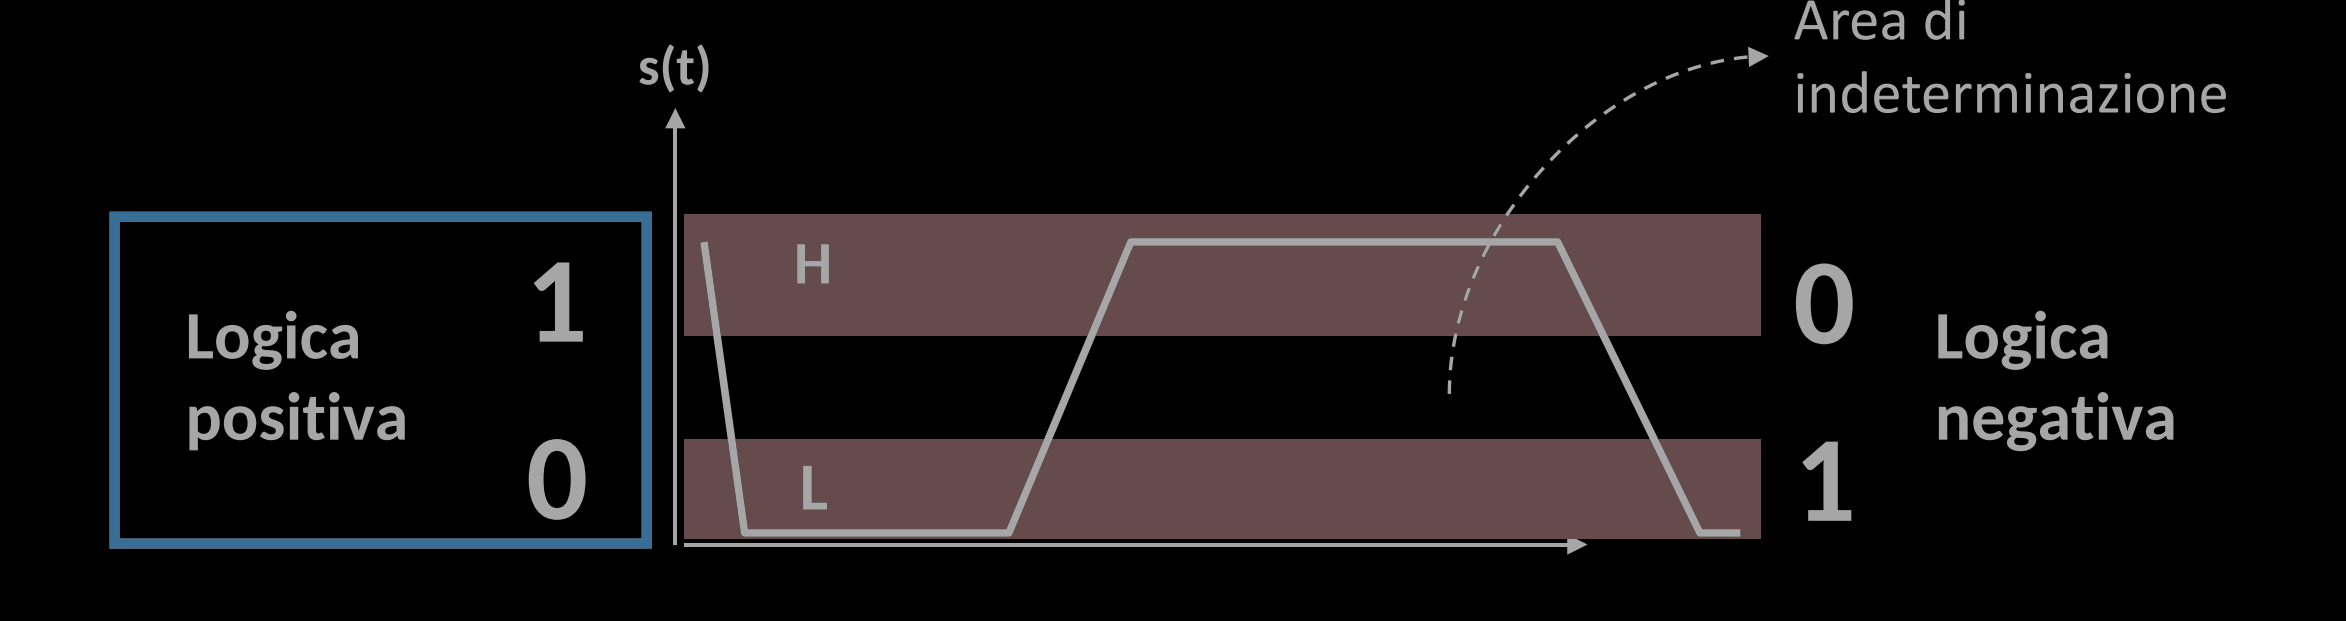
\includegraphics[scale=0.3]{logica.png}
\end{center}
\subsubsection*{Codici binari}
Per mantenere la robustezza del segnale binario, ma essere in grado di rappresentare più di due informazioni, usiamo una stringa (una sequenza) di segnali binari. Da precisare che una stringa di segnali binari può essere considerata un \textbf{codice binario} se e solo se chi genera la stringa e chi la "riceve" (nel senso che riceve l'informazione) si sono accordati in maniera adeguata sul significato.
\subsubsection{Codifica binaria dell'informazione}
Sappiamo che tutte le possibili permutazioni di 2 elementi di $n$ posizioni sono $2^n$.\\
Per esempio tutte le stringhe di 3 bit sono $8 = 2^3$. Mentre per rappresentare 7 colori bisogna risolvere una semplicissima disequazione:
$$ 2^n \geq 7 \rightarrow n \geq \log_2 7 = 2,807 = 3 $$
Per calcolare $n$ senza bisogno di risolvere il logaritmo, basta considerare la prima potenza di 2 maggiore del numero richiesto, il suo esponente è il numero di bit necessari.
\subsection{Interruttori}
Un bit può essere efficacemente generato e rappresentato dalla posizione di un interruttore (switch).
\subsubsection{Interruttore meccanico}
L'interruttore meccanico è formato semplicemente da una molla:
\begin{center}
    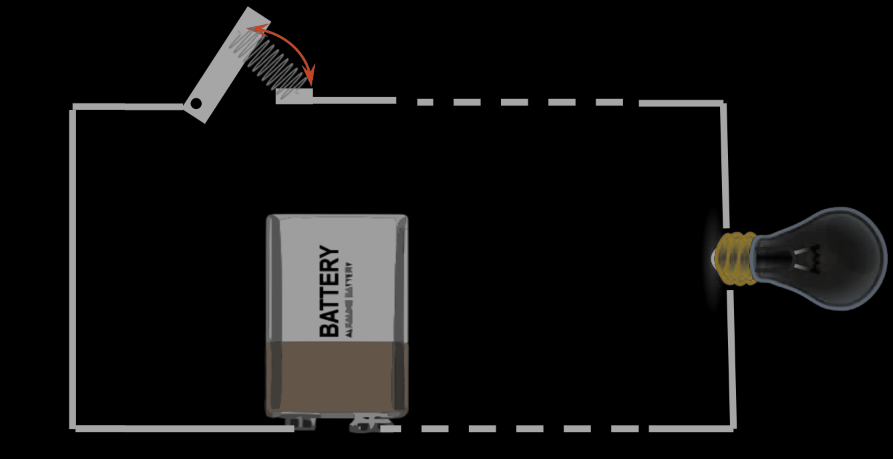
\includegraphics[scale=0.35]{intmecc.png}
\end{center}
\subsubsection{Interruttore elettronico}
Gli interruttori elettronici (transistor) sono molto più veloci e affidabili di quelli meccanici, e sono formati da un piccolo circuito la cui differenza di potenziale può oscillare tra 0 e 5 Volt:
\begin{center}
    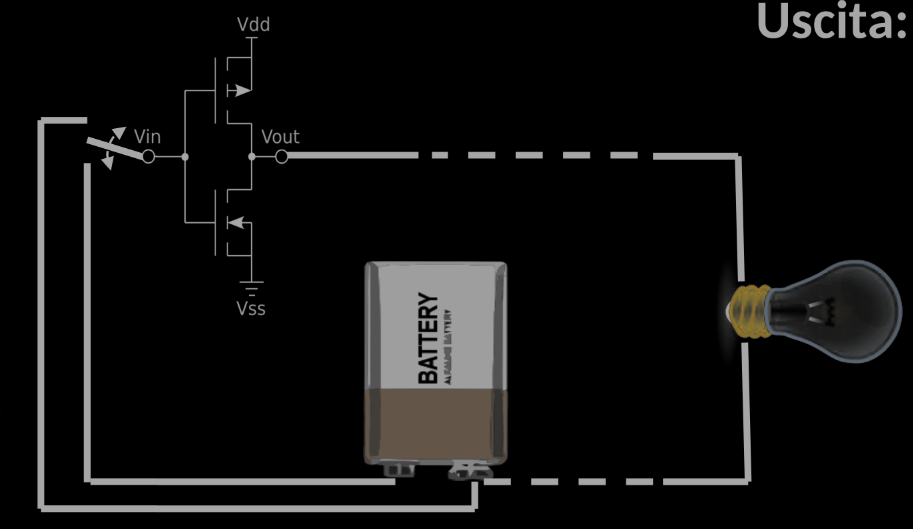
\includegraphics[scale=0.35]{intel.png}
\end{center}
Il grande vantaggio degli interruttori elettronici è di avere ingresso ed uscita della stessa natura, entrambe elettriche: è possibile usare l’uscita di un transistor per pilotarne altri, creando delle reti di interruttori che si influenzano e commutano senza intervento umano, e che possono essere realizzate in un circuito integrato
\subsection{Evoluzione della tecnologia}
\begin{itemize}
    \item La prima CPU Intel (4004) del 1971 conteneva circa 2300 transistor in grado di commutare (cambiare stato "aperto/chiuso") circa 700 mila volte ogni secondo
    \item La CPU AMD Ryzen 7 (2021) contiene quasi 11 Miliardi di transistor. Ciascuno può commutare miliardi di volte al secondo
    \item Le GPU Nvidia GA 100 Ampere (2020) possono contenere anche 54 Miliardi di transistor. Anche in questo caso in grado di commutare miliardi di volte al secondo
\end{itemize}
Ecco come, utilizzando tanti semplici interruttori, è possibile eseguire operazioni molto complesse.
\subsection{Livelli di astrazione}
Lavorare ad uno specifico livello di astrazione è una pratica standard di ogni ambito ingegneristico, in cui la descrizione di un sistema complesso è sempre articolata su più livelli. Ogni livello individua componenti “primitivi” la cui struttura è definita nel livello sottostante e di cui interessa solo il comportamento ("cosa può fare"), definito dalla sua interfaccia. Scopo di un livello è definire la struttura ("come è fatto") dei componenti primitivi usati dal livello soprastante. Esplorando i livelli della gerarchia dall’alto verso il basso, aumenta il numero di entità, ma diminuisce la complessità di ciascuna di esse.
\section{Introduzione alle Reti Logiche}
Una rete logica è quindi un'astrazione per una combinazione di interruttori (elettronici) che elaborano segnali binari.\\
Per astrarre dalla complessità della tecnologia sottostante si definiscono dei componenti elementari (gate, realizzati da interruttori elettronici) di cui ci interessa solo la relazione tra i segnali binari di ingresso e di uscita (comportamento).
\vspace{0.2cm}\\
In generale il numero di funzioni diverse di $n$ ingressi binari con un’uscita binaria è
$$ 2^{2^n} $$
I componenti elementari (cioè le funzioni) possibili limitandosi a quelli con un unico segnale binario di ingresso $x$ sono quindi 4, perché in questo caso abbiamo $n=4$
\begin{center}
    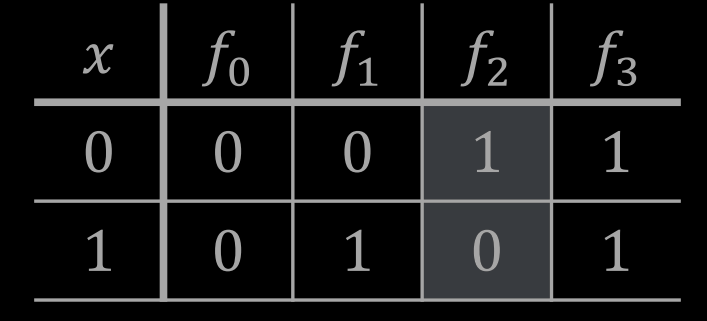
\includegraphics[scale=0.4]{funzioni1.png}
\end{center}
Tolte l’identità ($f_1$) e le costanti ($f_0$ e $f_3$), rimane un’unica funzione interessante, l’operatore NOT o invertitore ($f_2$).
\subsection{Vari tipi di gate}
\subsubsection{Il gate NOT}
Ogni gate elementare è descritto da
\begin{itemize}
    \item una tabella della verità, ovvero una tabella in cui ogni riga riporta una possibile configurazione degli ingressi e il valore dell’uscita ad essi corrispondente
    \item un simbolo circuitale, che astrae gli interruttori necessari ad implementare quel comportamento
    \item un’espressione, ovvero un modo di rappresentare la relazione tra ingressi ed uscite in forma compatta
\end{itemize}
Nel caso del gate NOT abbiamo:
\begin{center}
    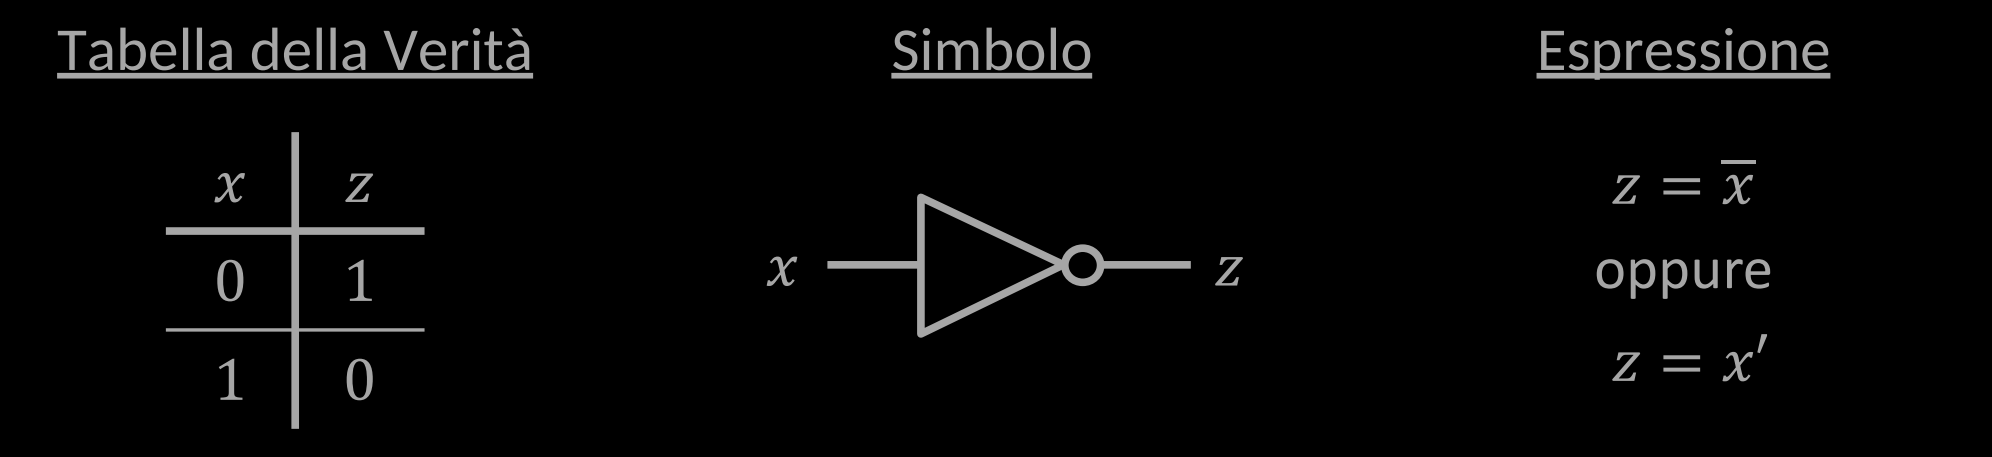
\includegraphics[scale=0.35]{desgate.png}
\end{center}
Usando la formula $2^{2^n}$con $n=2$ otteniamo che le possibili funzioni elementari di 2 ingressi sono 16
\begin{center}
    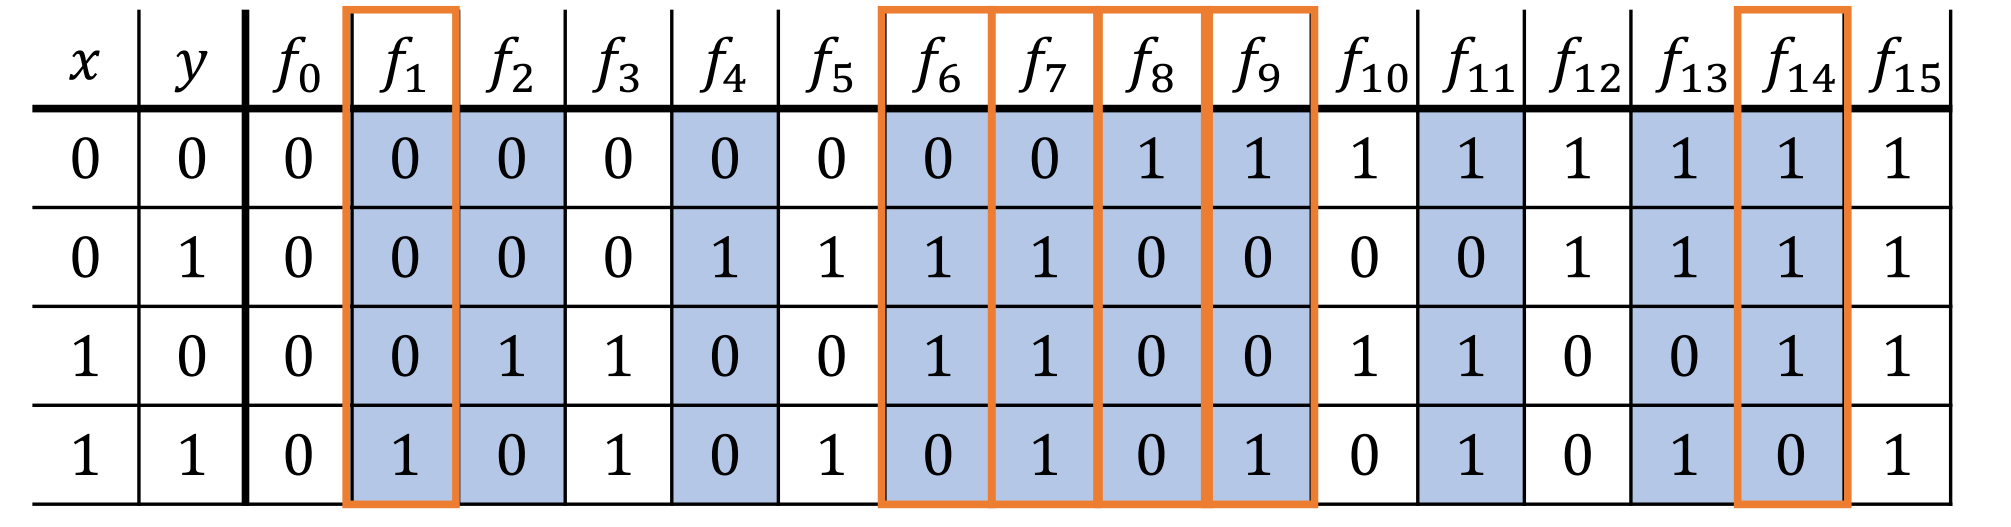
\includegraphics[scale=0.35]{funzioni2.png}
\end{center}
Tolte le costanti e le funzioni identità e NOT di ognuno dei due ingressi, rimangono 10 funzioni realmente di 2 ingressi, evidenziate in blu. Solo 6 sono disponibili come componenti elementari di reti logiche, quelle cerchiate in arancio, che sono descritte nelle pagine seguenti. Le altre non sono disponibili come componenti elementari: possono comunque essere realizzate a partire da quelle disponibili, come vedremo.
\subsubsection{Il gate AND}
Il componente AND è l’astrazione di due interruttori in serie. L’uscita assume valore logico 1 (la lampadina è accesa) se entrambe gli ingressi hanno valore 1, ovvero entrambi gli interruttori sono chiusi. 
\begin{center}
    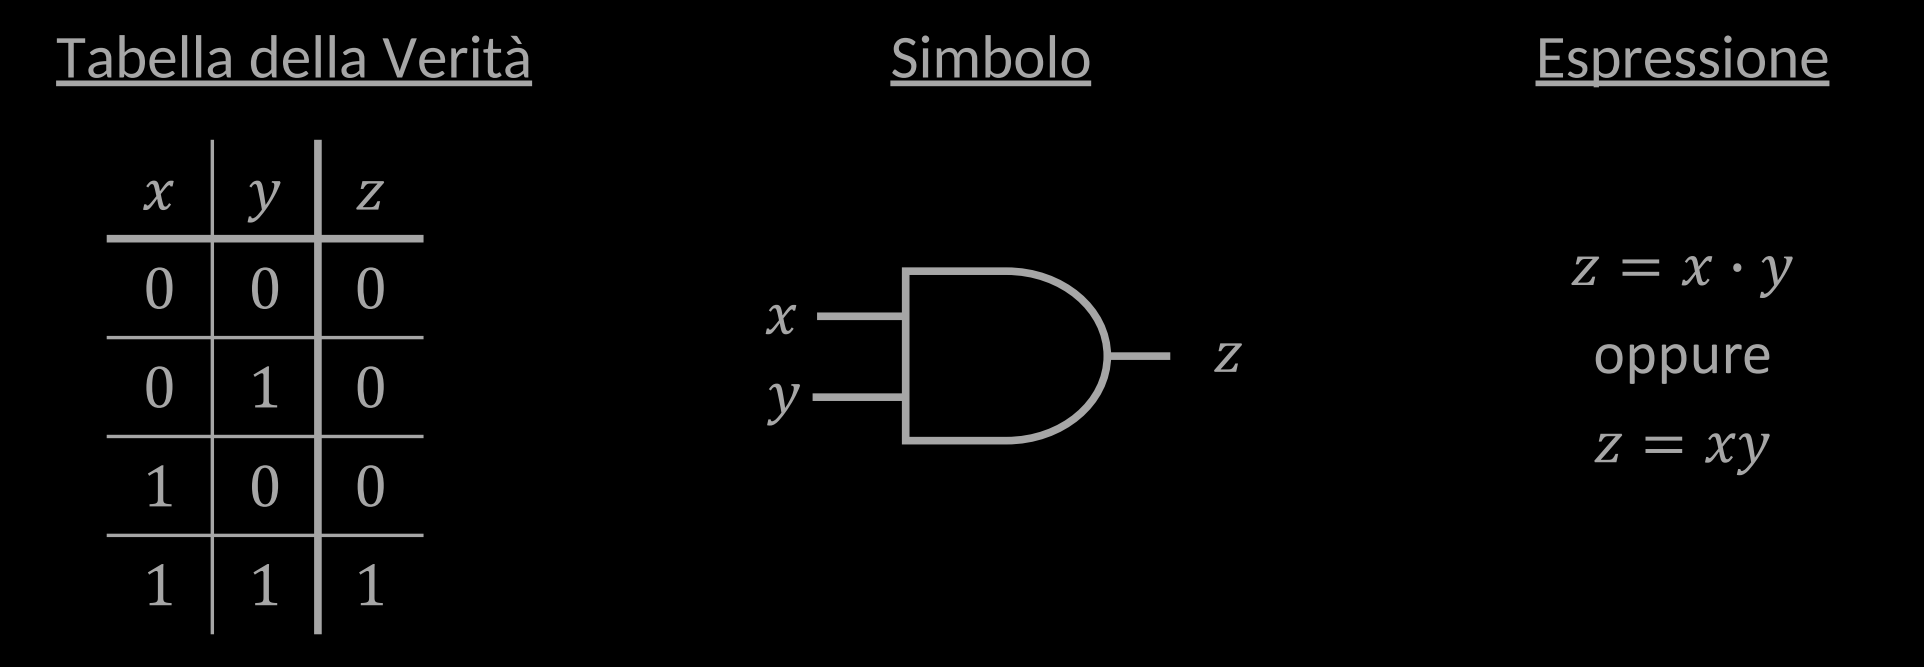
\includegraphics[scale=0.35]{desAND.png}
\end{center}
\subsubsection{Il gate OR}
Il componente OR è l’astrazione di due interruttori in parallelo. L’uscita assume valore logico 1 (la lampadina è accesa) se almeno un ingresso ha valore 1, ovvero almeno uno degli interruttori è chiuso.
\begin{center}
    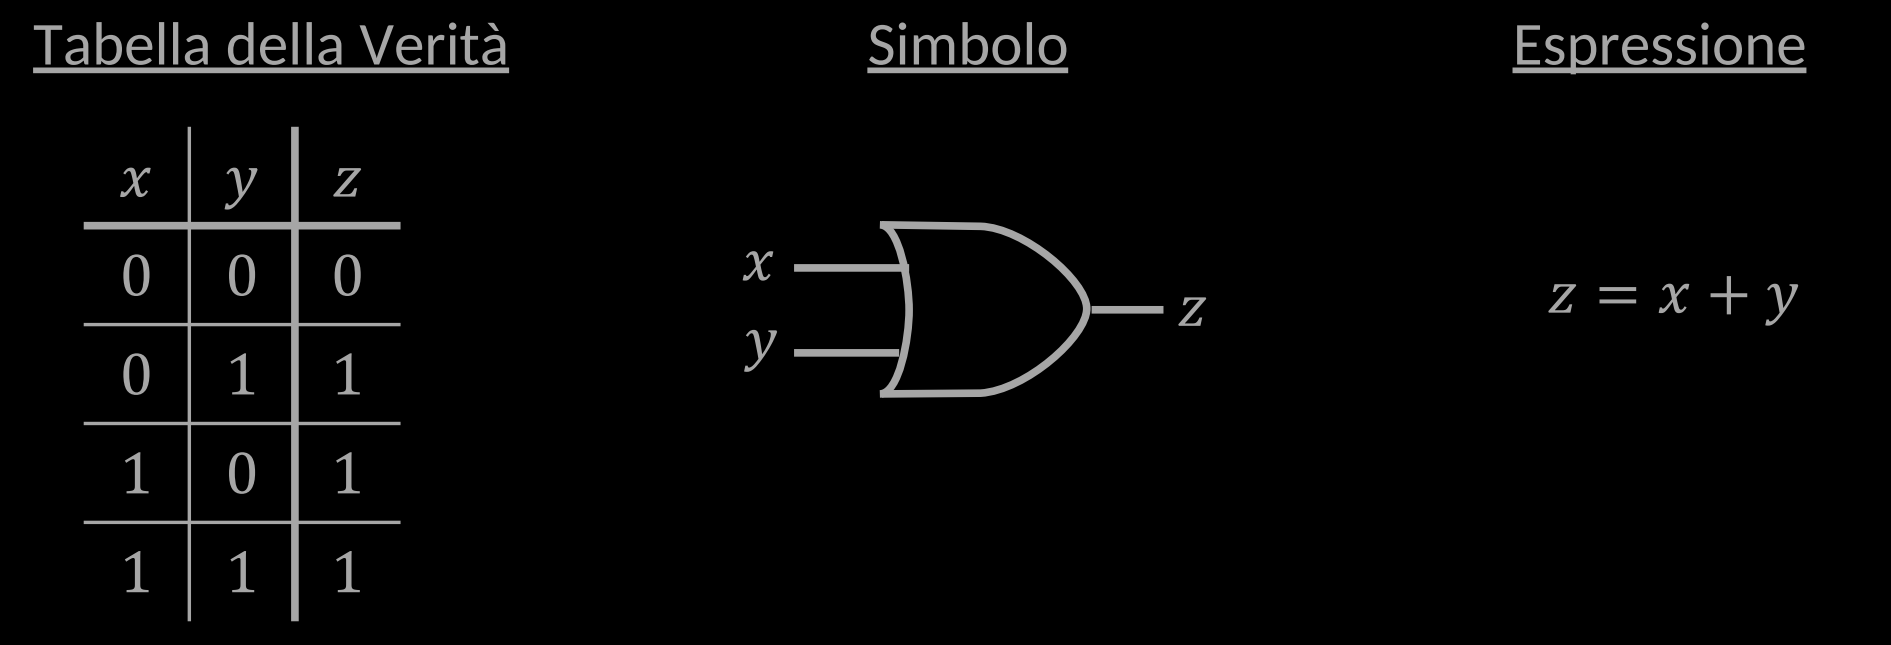
\includegraphics[scale=0.35]{desOR.png}
\end{center}
\subsubsection{AND e OR a più ingressi}
Dato il tipo di circuito di cui sono astrazione, risulta chiaro il comportamento di gate AND e OR a più di due ingressi. Per esempio, un AND a 3 ingressi corrisponde a 3 interruttori in serie: l’uscita vale 1 se e solo se tutti e 3 gli ingressi hanno valore 1.\\
Il numero di ingressi di un gate viene detto il suo \textbf{fan-in}.
\vspace{0.2cm}\\
La rappresentazione di un gate con 3 ingressi è un po' più complessa delle altre viste finora:
\begin{center}
    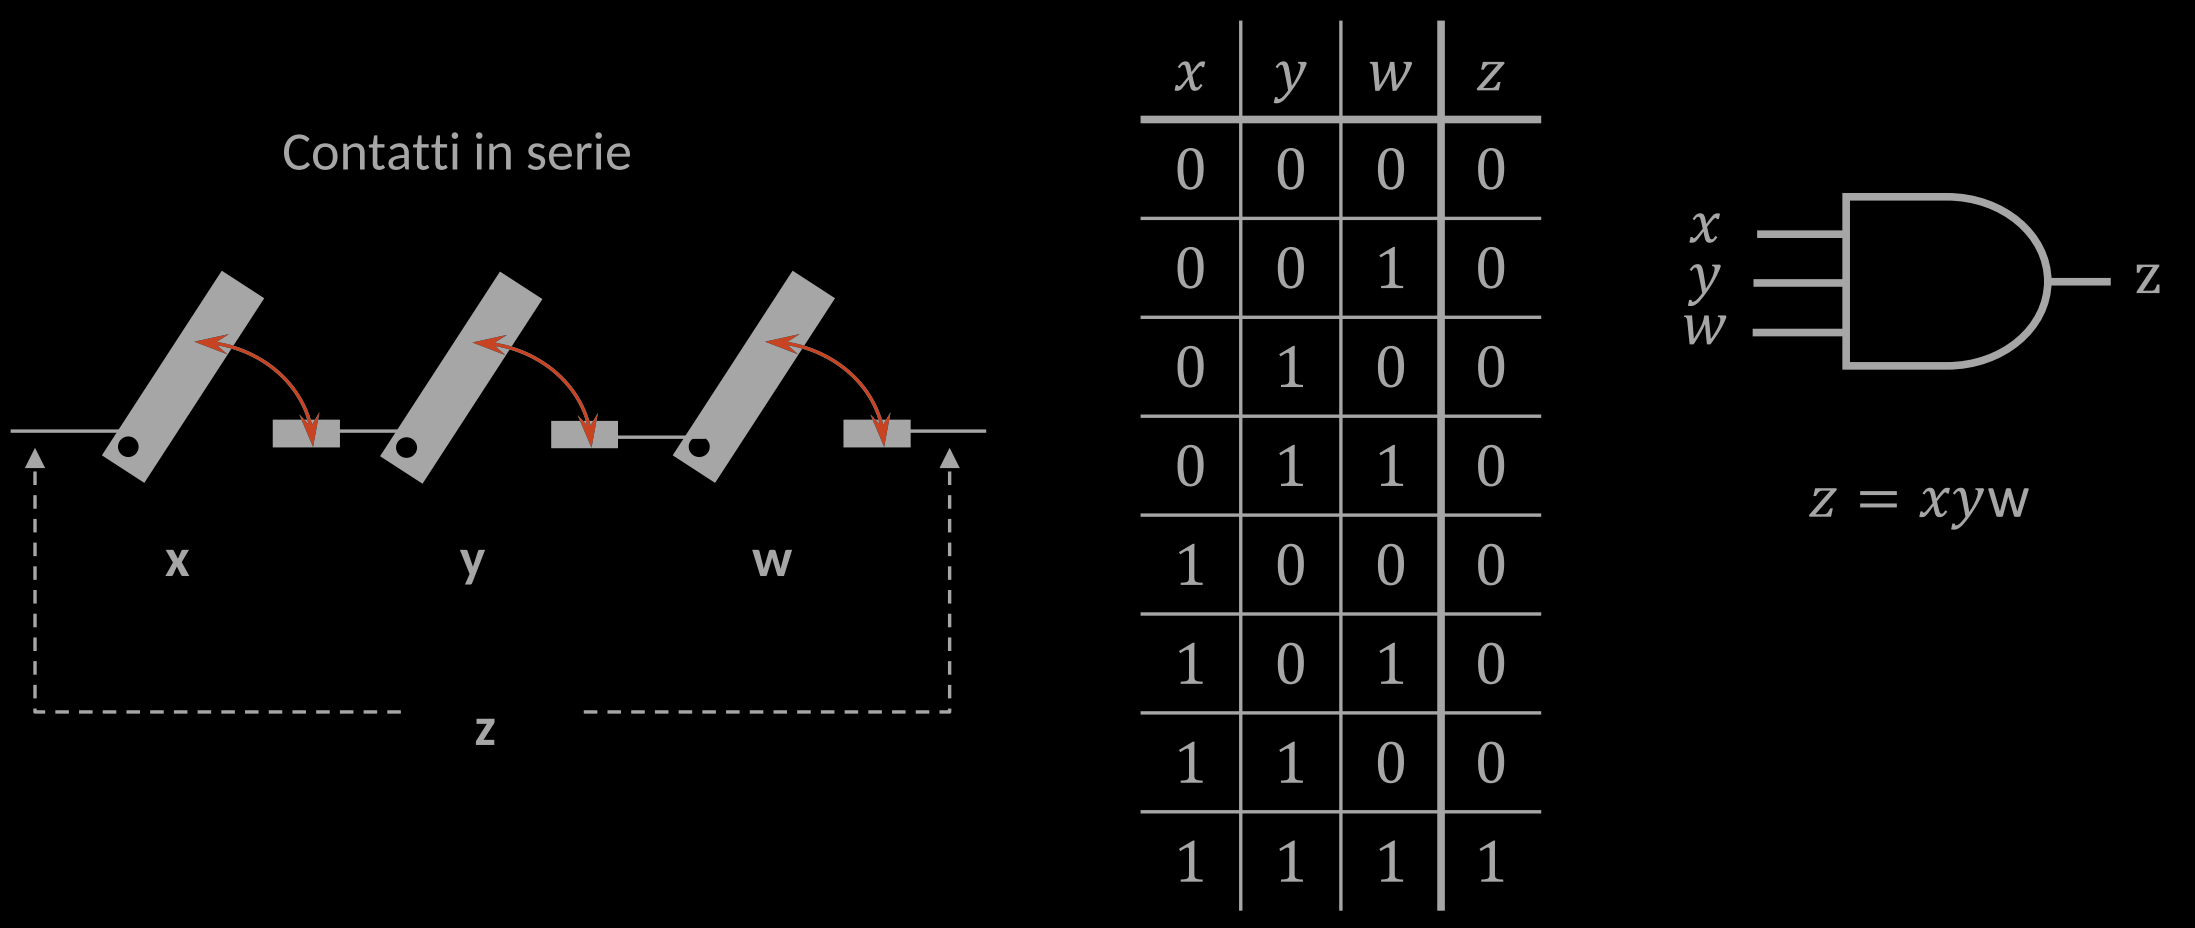
\includegraphics[scale=0.35]{desGate3.png}
\end{center}
\subsubsection{Il gate EXOR}
Il componente EXOR è l’astrazione di due deviatori, ovvero interruttori che chiudono il circuito verso uno di due possibili percorsi. L’uscita assume valore logico 1 (la lampadina è accesa) se un ingresso ha valore 1 ma non entrambi, ovvero i due deviatori sono su posizioni diverse.
\begin{center}
    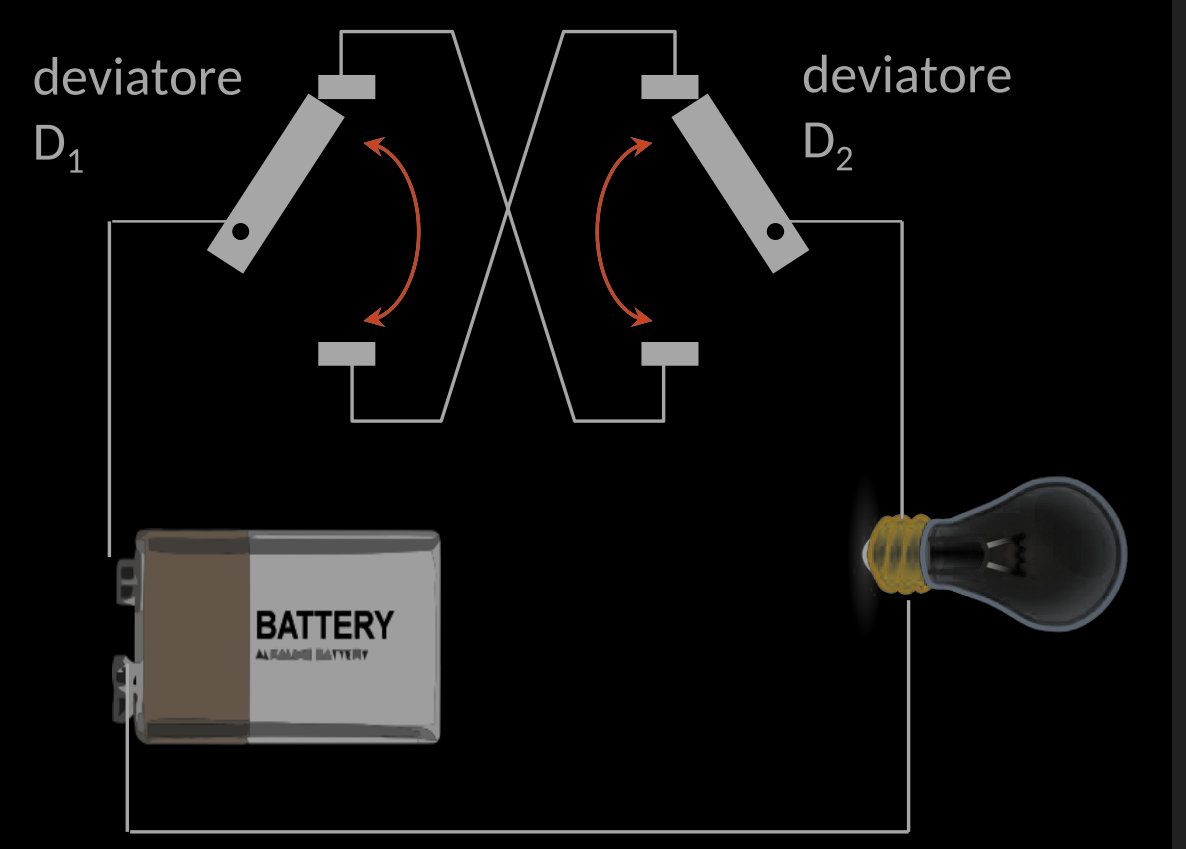
\includegraphics[scale=0.35]{circEXOR.png}
    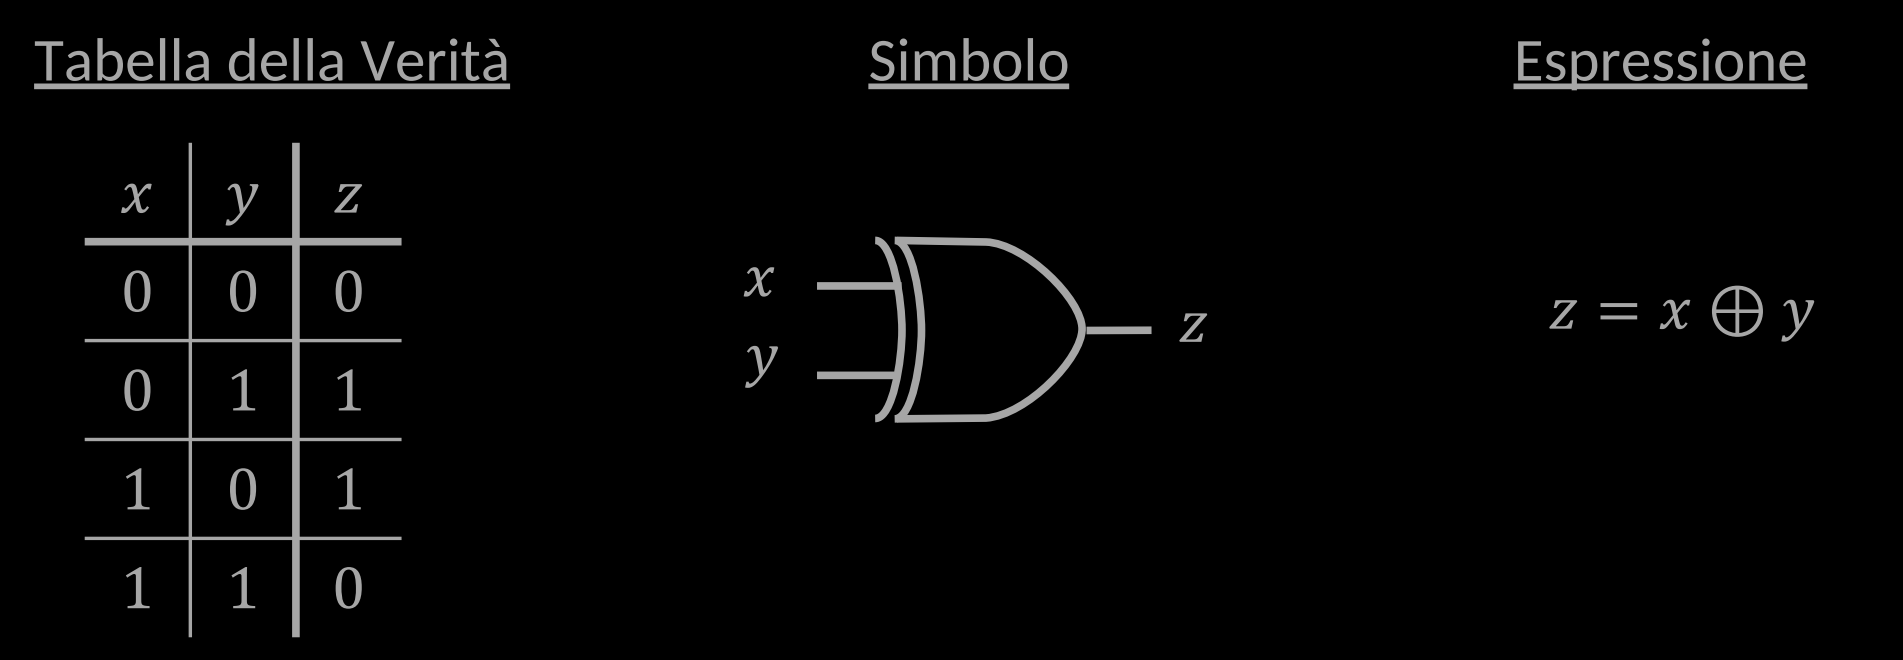
\includegraphics[scale=0.35]{desEXOR.png}
\end{center}
\subsubsection{Comportamento del gate EXOR/XOR}
Il nome di questo gate deriva dalla contrazione del nome exclusive OR, infatti esso può assumere valore uno solo se uno dei due ingressi ha valore 1. L’operatore EXOR viene anche detto somma modulo 2, in quanto il suo output può essere interpretato come il risultato della somma (escluso il riporto) di due bit. \\
Si può anche interpretare lo XOR come controllo sul numero 1: esso vale 1 se e solo se il numero di 1 in ingresso è dispari.\\
Con quest’ultima interpretazione si può facilmente estendere il gate EXOR a più ingressi, anche se è meno comune farne uso rispetto a AND e OR.
\subsubsection{I gate NAND, NOR e EXNOR}
\begin{center}
    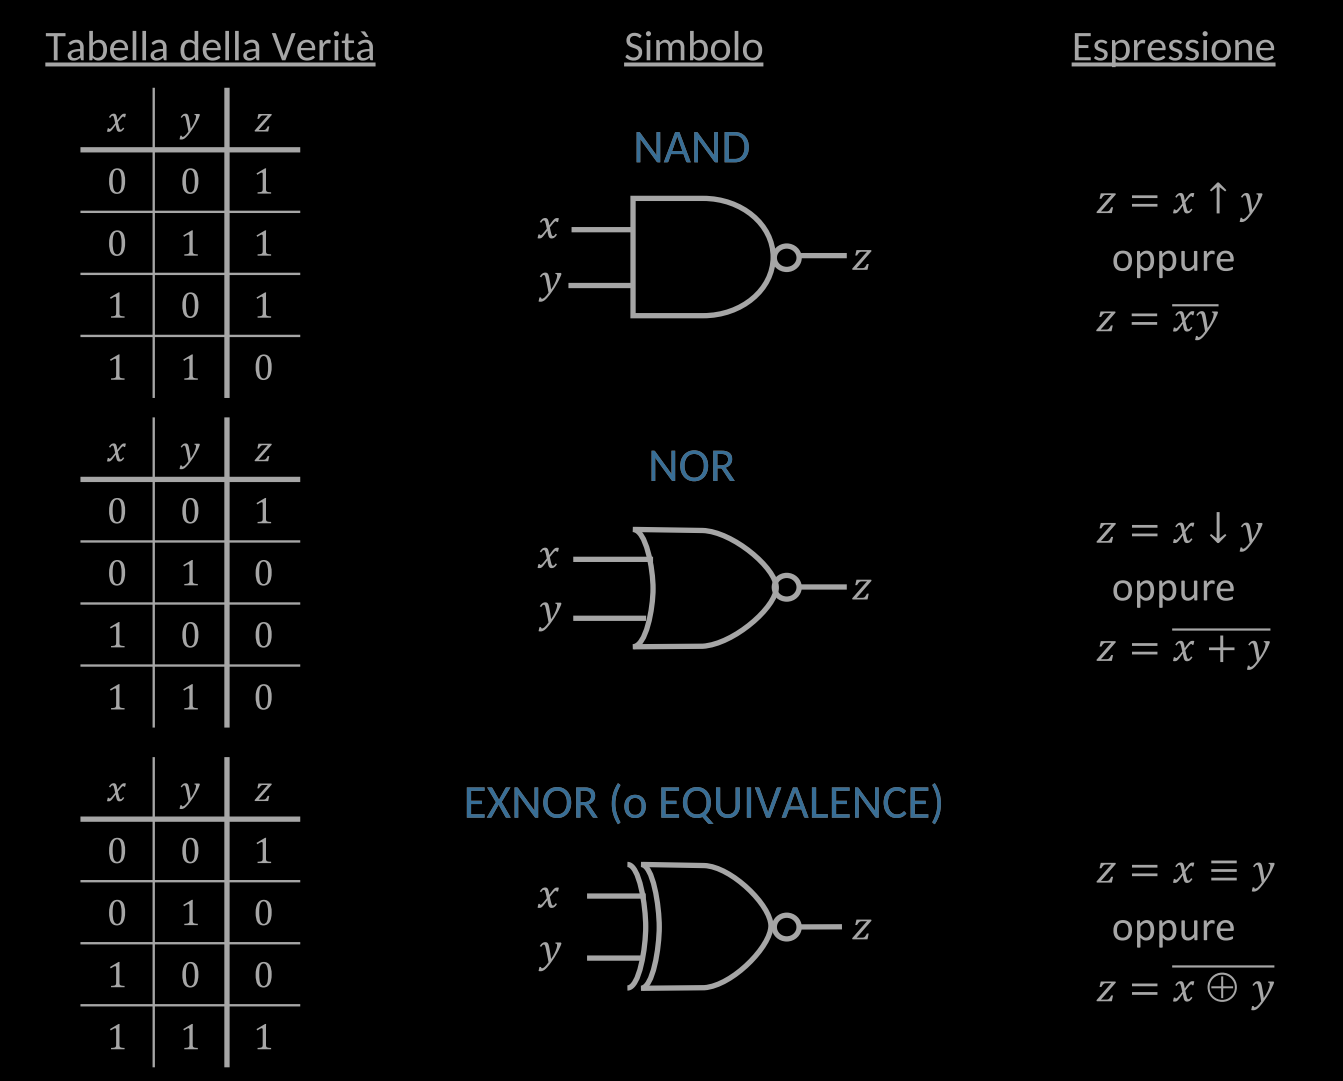
\includegraphics[scale=0.43]{nand.png}
\end{center}
Il gate EXNOR viene anche chiamato EQUIVALENCE perché, per due ingressi, ho uscita 1 solo se i due ingressi sono uguali.
\vspace{0.2cm}\\
I tre gate sono le versioni negate dei gate definiti in precedenza, quindi l’estensione a più ingressi si può ricavare negando quella di AND, OR e EXOR: per esempio un NAND a 4 ingressi ha uscita 0 solo quando tutti e 4 gli ingressi valgono 1, uscita 1 altrimenti. Essendo ottenibili dai gate precedenti con un NOT in cascata non sarebbero strettamente necessari, ma hanno proprietà che li rendono utili e che vedremo in seguito.
\subsection{Diagrammi ad occhio}
Per rappresentare l’evoluzione di gruppi di segnali binari in forma compatta, per esempio gli ingressi di un gate (o di una rete più complessa), si usano i cosiddetti diagrammi ad occhio. Poiché i segnali analogici sottostanti non cambiano valore istantaneamente, il diagramma riporta anche i transitori tra una configurazione stabile e la successiva.
\begin{center}
    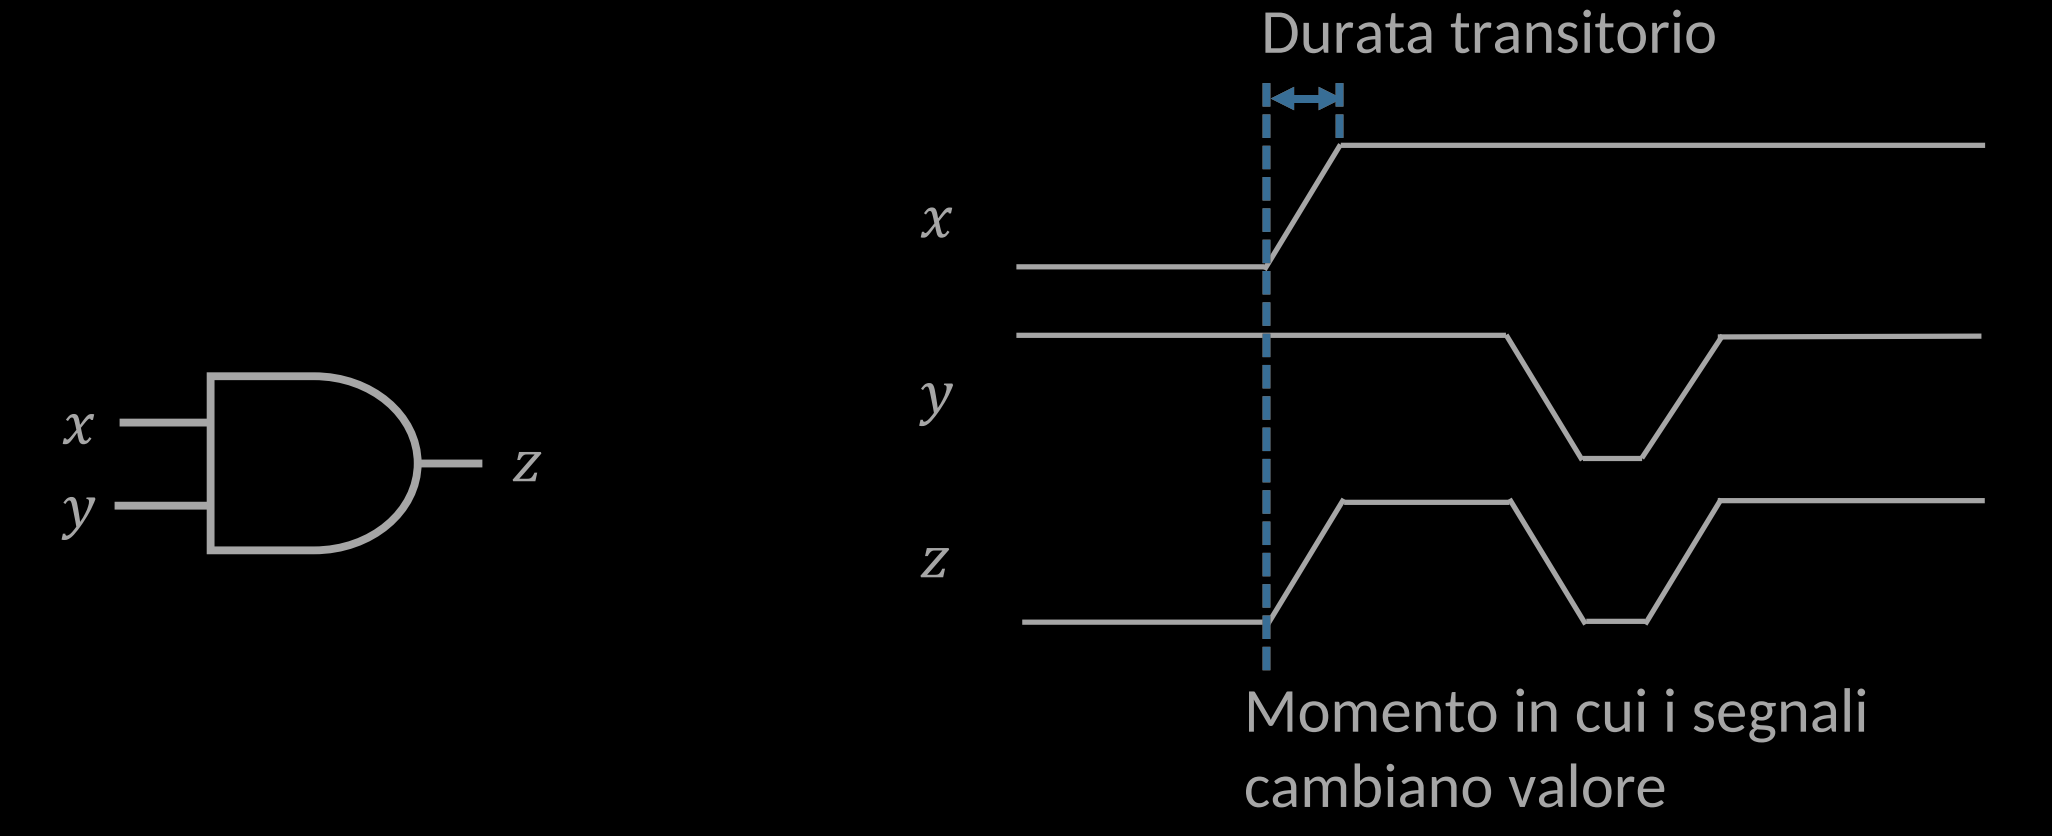
\includegraphics[scale=0.33]{diagrammiocchio.png}
\end{center}
\subsubsection{Bus di segnali}
L’evoluzione di un gruppo di bit può anche essere descritta scrivendone la configurazione binaria nel diagramma.\\
Un insieme di segnali viene anche detto un \textbf{bus}. Per indicare un bus di $n$ segnali che codificano un’informazione, useremo anche la notazione con parentesi quadre [$n-1$ . . 0].
\begin{center}
    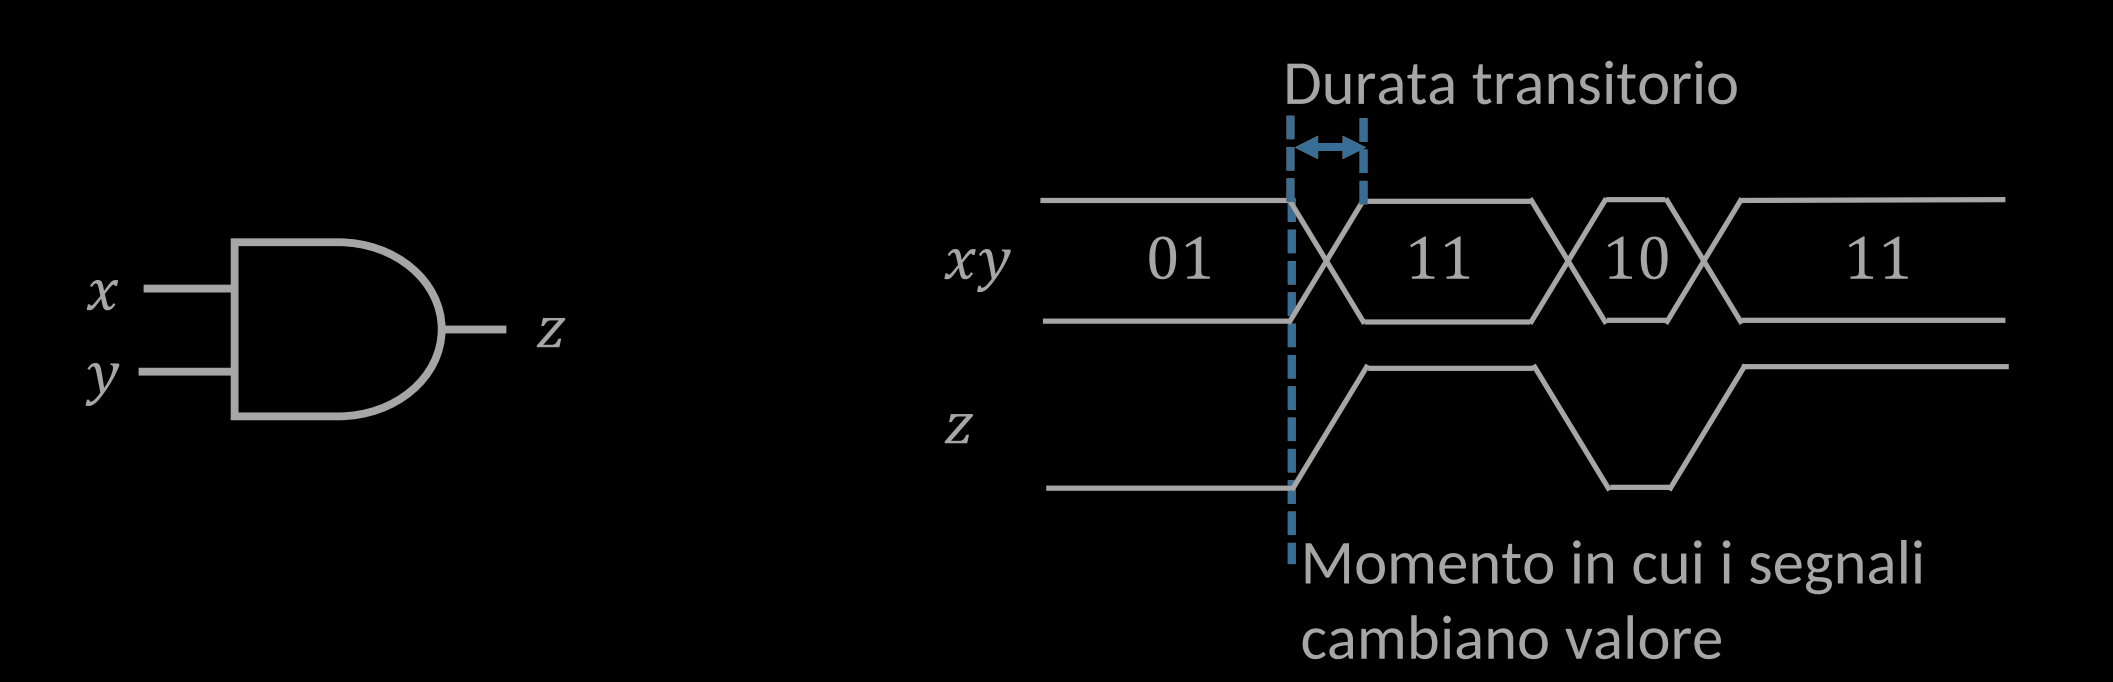
\includegraphics[scale=0.35]{diagrammabus.png}
\end{center}
\subsubsection{Ritardi di propagazione}
Anche se stiamo astraendo dagli interruttori sottostanti per rendere gestibile il progetto e l’analisi, dobbiamo sempre ricordare che i gate sono anche componenti reali. La differenza principale tra l’astrazione fornita dalla tabella della verità e un gate reale è il ritardo di propagazione. Quando cambia un ingresso di un gate, l’uscita non cambia istantaneamente, ma dopo un tempo $\tau_p$ che dipende dalla tecnologia utilizzata.\\
Il ritardo di propagazione non è solo un semplice ritardo puro, ma un ritardo "inerziale": un impulso di durata inferiore a $\tau_p$ su uno degli ingressi non appare in uscita. Esiste quindi un limite superiore per la velocità di funzionamento di ogni gate.
\begin{center}
    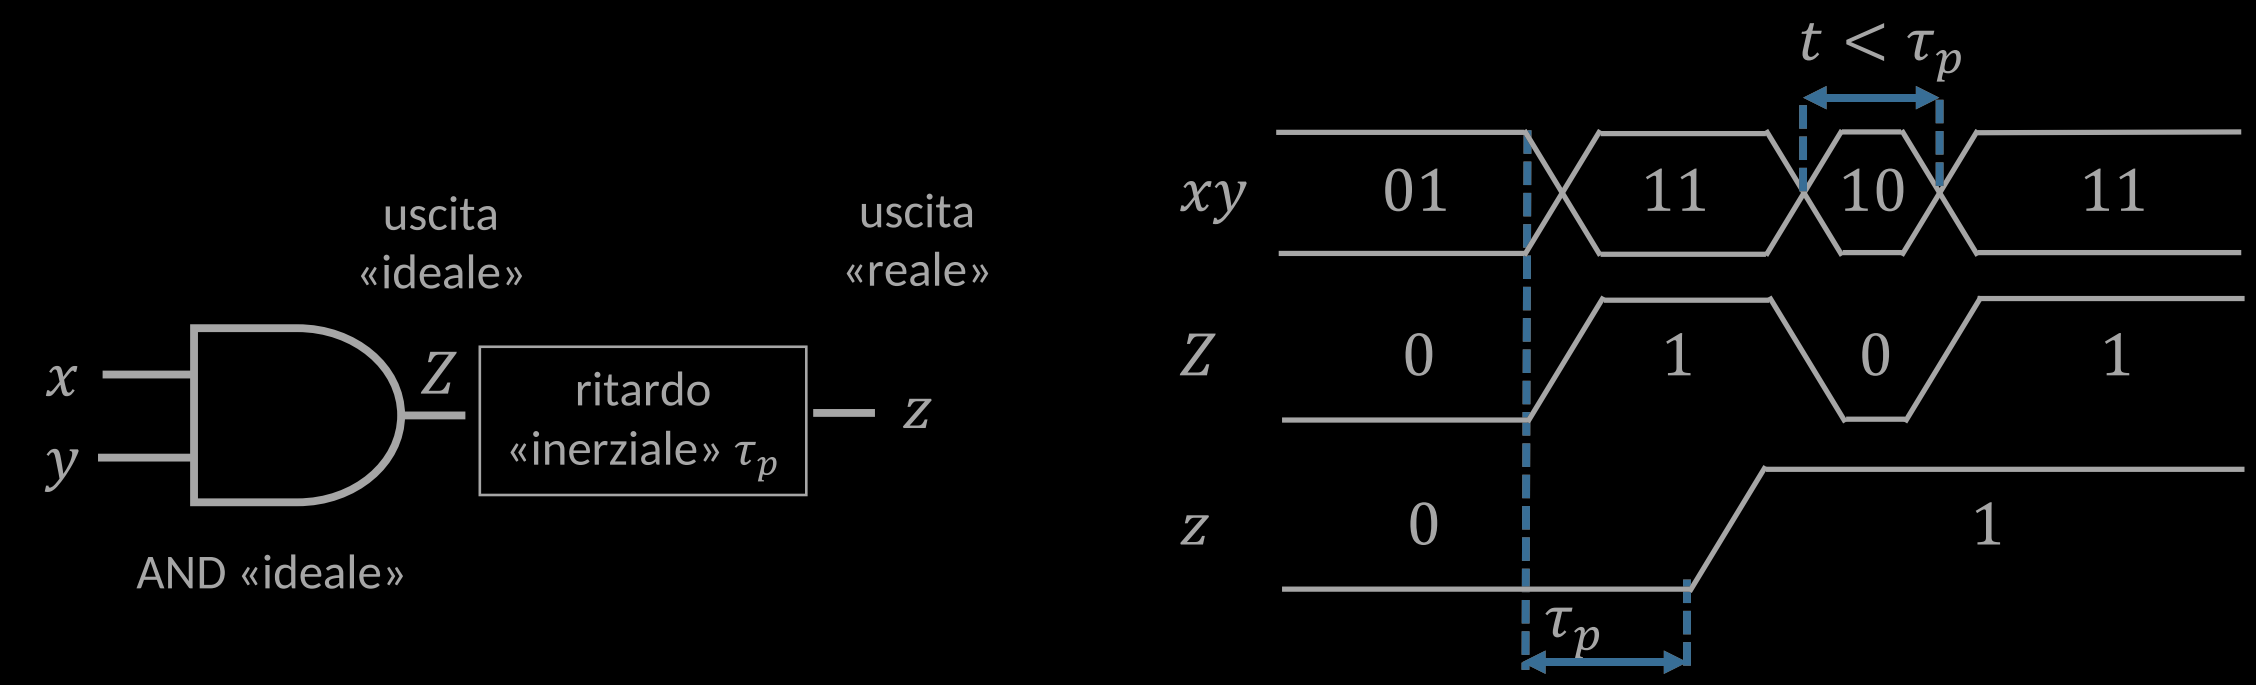
\includegraphics[scale=0.35]{ritardi.png}
\end{center}
\subsection{Montaggio tra gate}
Dati due gate (o gruppi di gate), è possibile montarli in tre modi:
\begin{itemize}
    \item In serie, ovvero l’uscita del gate a monte è uno degli ingressi del gate a valle
    \begin{center}
        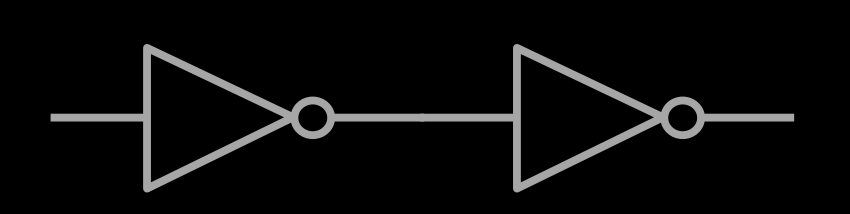
\includegraphics[scale=0.35]{gateinserie.png}
    \end{center}
    \item In parallelo, ovvero alcuni degli ingressi sono in comune (e non le uscite)
    \begin{center}
        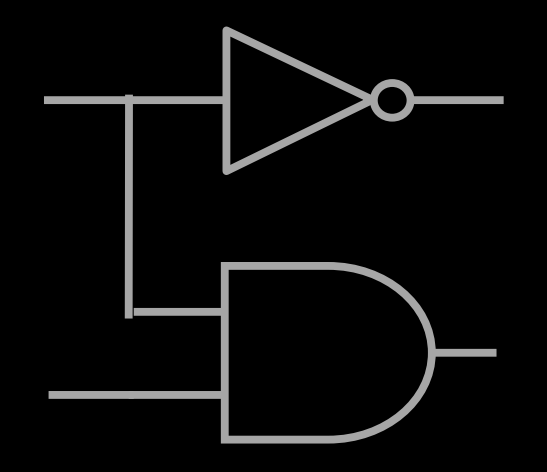
\includegraphics[scale=0.35]{gateinparallelo.png}
    \end{center}
    \item In retroazione, ovvero l’uscita di un gate è uno degli ingressi dell’altro e viceversa
    \begin{center}
        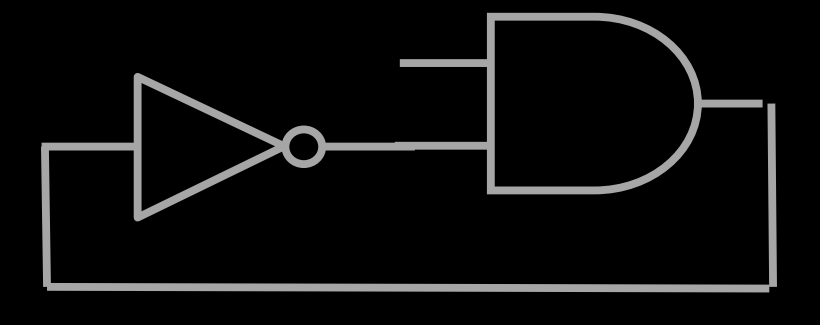
\includegraphics[scale=0.35]{gateinretro.png}
    \end{center}
\end{itemize}
\textbf{N.B.} non si possono collegare tra loro uscite di gate.
\subsection{Conversione A/D e D/A}
Abbiamo visto che è conveniente rappresentare l’informazione sotto forma di stringhe di segnali binari. Input e output possono però essere anche segnali analogici: si rende quindi necessario per alcuni segnali operare conversioni da analogico a digitale (A/D) e viceversa (D/A).\\
Ne sono un esempio le foto, in cui si converte un segnale analogico (la luce).
\section{Rappresentazione dell'informazione}
Una macchina digitale elabora e comunica \textbf{informazione}. Una definizione molto generale di informazione è la seguente: una stringa di lunghezza finita di simboli appartenenti ad un alfabeto.
\subsection{Codifica binaria dell'informazione}
L’utilizzo di segnali binari per l’elaborazione e la comunicazione di una macchina digitale comporta che
\begin{itemize}
    \item la macchina impieghi un alfabeto binario (ovvero che utilizzi i due soli simboli: 0 e 1)
    \item qualsiasi informazione elaborata o comunicata sia rappresentata da una \textbf{stringa di bit}
\end{itemize}
\subsubsection{Codice binario}
\textbf{Definizione:} Funzione dall’insieme delle $2^n$ configurazioni di $n$ bit ad un insieme di $M$ informazioni (simboli alfanumerici, colori, numeri, ecc.).
\vspace{0.2cm}\\
La condizione necessaria per la codifica è che il numero di configurazioni di bit possibili sia uguale o superiore al numero di informazioni:
$$ 2^n \geq M $$
\subsubsection*{Proprietà di un codice}
Un codice è una rappresentazione convenzionale dell'informazione. \\
La scelta di un codice deve essere condivisa da sorgente e destinazione, ed ha due gradi di libertà:
\begin{itemize}
    \item il numero n di bit (qualsiasi, purché $2^n \geq M$)
    \item l’associazione tra configurazioni e informazioni
\end{itemize}
\vspace{0.2cm}
A parità di $2^n$ e di $M$, le associazioni possibili (disposizioni senza ripetizione) sono:
$$ C = 2^n! / (2^n - M)! $$
\subsubsection*{Esempi}
\begin{align*}
&n=1, M=2 \rightarrow C = 2\\
&n=2, M=4 \rightarrow C = 24\\
&n=3, M=8 \rightarrow C = 40.320\\
&n=4, M=10 \rightarrow C = 29.059.430.400
\end{align*}
\subsubsection{Codici ridondanti}
Poiché la condizione per rendere possibile la codifica di $M$ informazioni è $2^n \geq M$, il \textbf{numero minimo} di bit necessari per creare un codice che rappresenti $M$ informazioni è
$$n_{min} = \log_2 M $$
Un codice che utilizza esattamente $n_{min}$ bit è detto \textit{codice non ridondante}. Invece un codice che utilizza $n > n_{min}$ bit è detto \textit{codice ridondante}.
\subsection{Rappresentazione posizionale}
In una generica base $\beta$ avrò $\beta$ cifre possibili: per basi con $\beta \leq 10$ si usano le cifre tradizionali, per basi con $\beta > 10$ si usano in aggiunta ai numeri dei caratteri come cifre aggiuntive (A,B,C,...).\\
Per calcolare il valore del numero rappresentato si sommano i numeri naturali corrispondenti alle cifre, moltiplicati per una potenza di $\beta$ che dipende dalla \textbf{posizione}:
$$ N = (n_{n-1}\beta ^{n-1} + ... + n_0\beta^0 + n_{-1}\beta^{-1} + ... + n_{-m}\beta^{-m})  $$
\subsubsection*{Esempi}
\begin{center}
    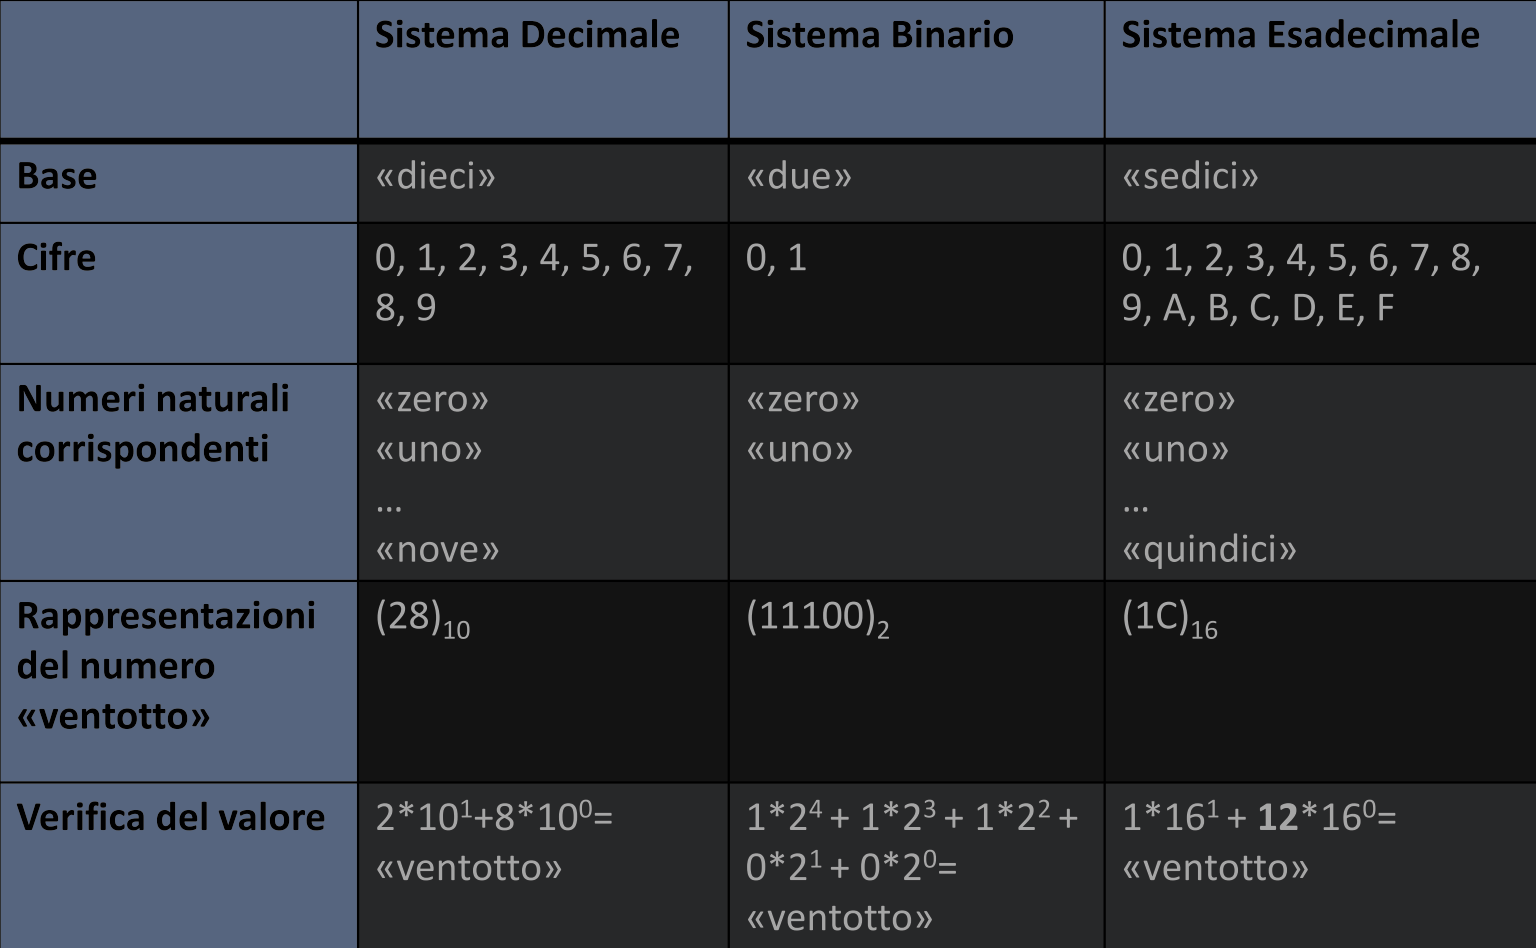
\includegraphics[scale=0.38]{espos.png}
\end{center}
\subsubsection{Cambio di base da 2 a 16}
La base 16 è spesso usata per rappresentare lunghe stringhe di numeri binari in forma compatta (per esempio indirizzi di memoria in un calcolatore). Il cambio di base tra questi due sistemi è semplice: ad ogni gruppo di 4 cifre binarie corrisponde un simbolo esadecimale e viceversa, per esempio:
\begin{center}
    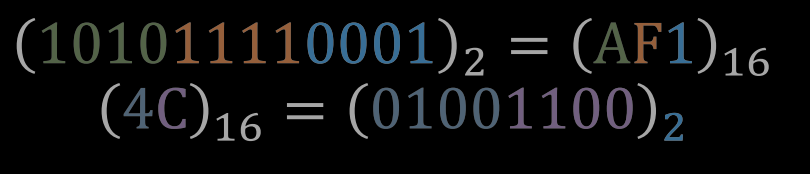
\includegraphics[scale=0.35]{esEs.png}
\end{center}
In generale il cambio di base da una generica $\beta$ a un'altra base $\beta^*$ non è immediato, ma a noi interessano solo due casi notevoli:
\begin{itemize}
    \item conversione da binario/esadecimale a decimale: è sufficiente calcolare il valore di un numero tramite l’espansione polinomiale che abbiamo visto per averne anche la rappresentazione in base 10;
    \item conversione da decimale a binario/esadecimale: metodo di conversione iterativa descritto tramite esempi che vedremo in seguito.
\end{itemize}
\subsubsection{Esempio di conversione iterativa}
Supponiamo di voler convertire $(41,6875)_{10}$ in binario:
\begin{center}
    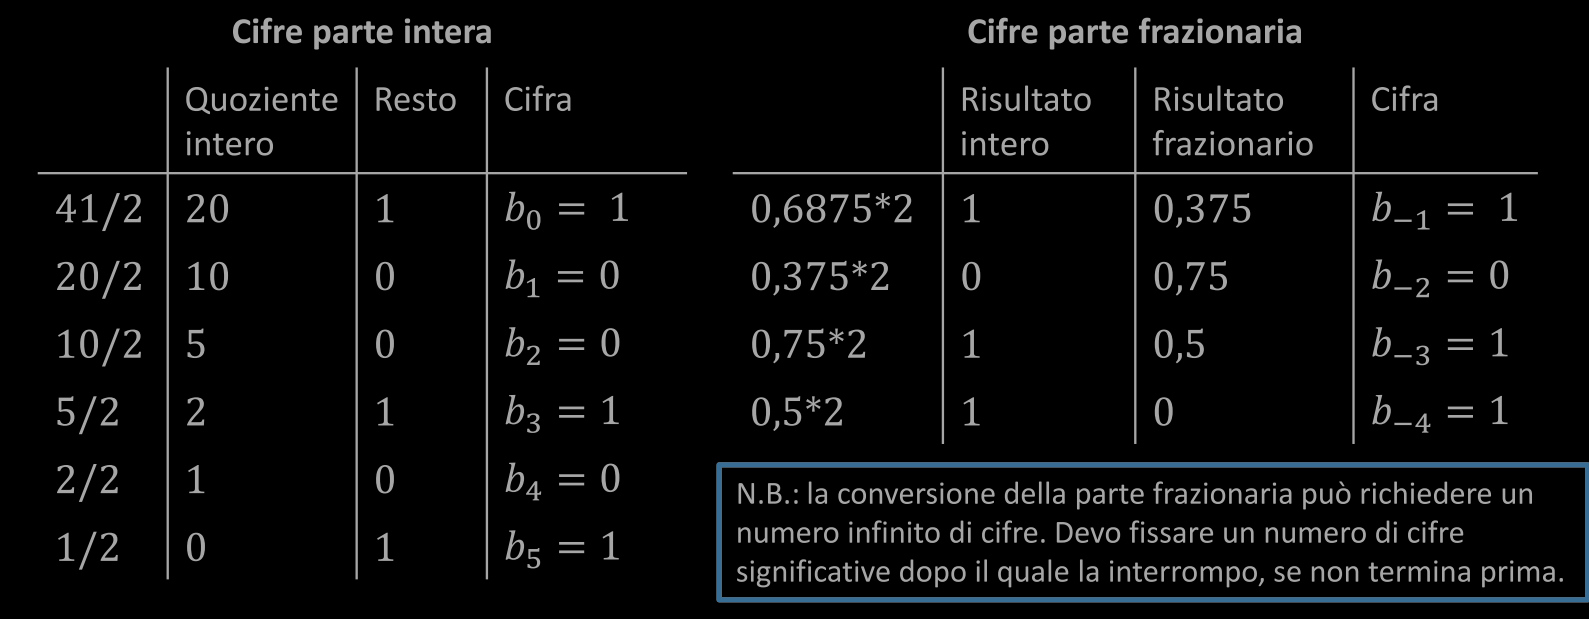
\includegraphics[scale=0.4]{esIter.png}
\end{center}
La rappresentazione cercata è quindi $(101001,1011)_2$
\par\noindent\rule{\textwidth}{0.4pt}
Proviamo ora invece a convertire $(41,6875)_{10}$ in esadecimale:
\begin{center}
    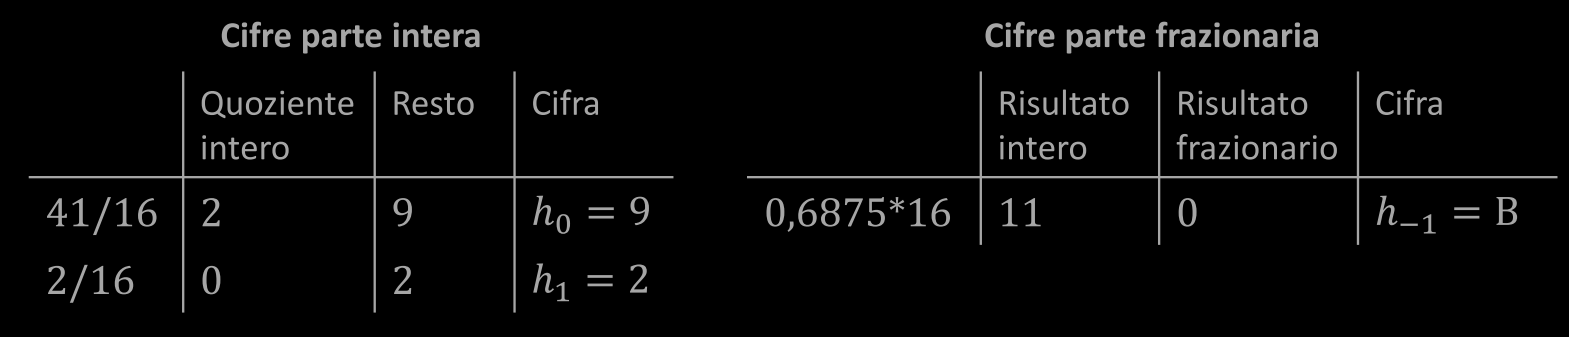
\includegraphics[scale=0.35]{esIterEs.png}
\end{center}
La rappresentazione cercata è quindi $(29,B)_{16}$
\subsubsection{Numeri binari senza segno}
Per rappresentare un numero senza segno N in una macchina digitale si usa quindi la rappresentazione in base 2. Dati $n$ bit, i numeri senza segno rappresentabili sono compresi tra $0$ e $2^{n} - 1$.\\
Esempio: in C, il tipo {\fontfamily{lmtt}\selectfont unsigned short} ha (tipicamente) dimensione 16 bit, i numeri rappresentabili appartengono quindi all’intervallo [0,65.535].
\subsection{Conversione di codice (trascodifica)}
\begin{center}
    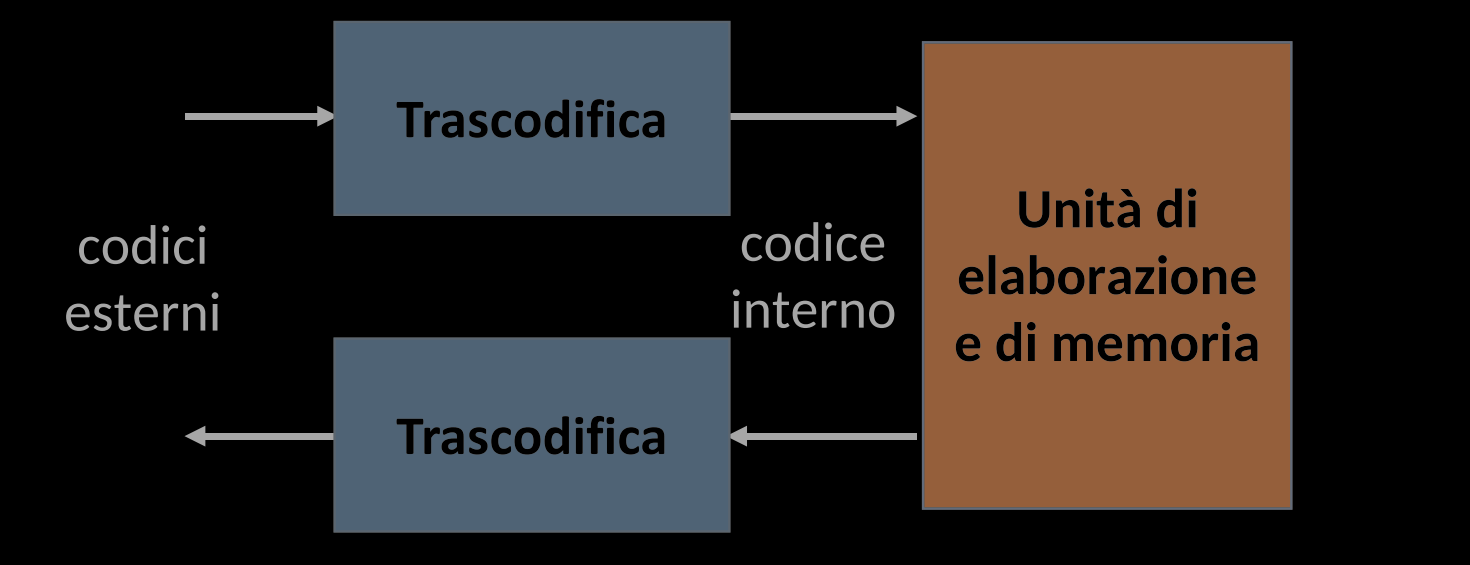
\includegraphics[scale=0.33]{trascod.png}
\end{center}
Il \textbf{codice interno} è di norma non ridondante per minimizzare il numero di bit da elaborare e da memorizzare.\\
Il codice esterno è di norma:
\begin{itemize}
    \item ridondante per semplificare la generazione e l'interpretazione delle informazioni;
    \item standard, per rendere possibile la connessione di macchine (o unità di I/O) realizzate da costruttori diversi.
\end{itemize}
\subsubsection{Codici proprietari e codici standard}
\textbf{Codice proprietario:} codice scelto da un Costruttore per mettere in comunicazione macchine di sua produzione. L'uso di codici proprietari mira ad ottimizzare le prestazioni e a proteggere il mercato di certe macchine. Ne sono esempi il Linguaggio Assembler o il telecomando della TV o del condizionatore.
\vspace{0.1cm}\\
\textbf{Codice standard:} codice scelto da norme internazionali (de iure) o dal costruttore di una macchina ampiamente utilizzata sul mercato (de facto). L'uso di codici standard nelle unità di I/O consente di collegare macchine realizzate da Costruttori diversi. Un esempio sono le stampanti che si interfacciano con qualsiasi calcolatore.
\subsubsection{Esempio dell'ascensore}
Immaginiamo un ascensore che serve 4 piani;\\
I \textbf{segnali in ingresso} sono:
\begin{itemize}
    \item presenza o meno della cabina a uno dei piani (4 rilevatori di presenza, 5 casi possibili perché bisogna contare anche il caso in cui l'ascensore sta salendo e non si trova in nessun piano, cioè il caso nullo);
    \item richiesta di spostamento della cabina (pulsantiera a 4 tasti, 5 casi possibili);
\end{itemize}
Quindi in entrambi i casi si ha n=4, M=5 e avremo un codice ridondante.
\vspace{0.2cm}\\
\textbf{Segnali in uscita:}
\begin{itemize}
    \item indicatore del piano corrente ai vari piani e in cabina (4 lampade, 5 casi possibili);
\end{itemize}
Anche in questo caso n=4, M=5 e avremo un codice ridondante.
\subsection{Codici standard}
\subsubsection{Codice ASCII esteso (8 e 16 bit)}
\begin{itemize}
    \item Estensione del codice ASCII a 8 bit, includendo nell’insieme dei caratteri
    rappresentati i simboli impiegati dalle lingue originate dal latino (in Europa…);
\item Standard Unicode (fino al 1995): ulteriore estensione (16 bit) che aveva lo scopo di
permettere di codificare in binario con 2 byte i simboli di tutte le lingue conosciute;
\item Standard Unicode 2.0 e seguenti(dal 1996): lo spazio Unicode è stato ulteriormente
esteso e adesso è un codice a 21 bit.
\end{itemize}
\subsubsection{UTF}
Le architetture e i linguaggi di programmazione sono progettati e ottimizzati per operare su gruppi di byte (= 8 bit) che seguono le potenze di 2, ovvero 1 byte, 2 byte, 4 byte, etc...\\
Sono stati quindi definiti 3 standard per mappare un carattere Unicode da 21 bit in una sequenza di byte non ridondanti (ovvero farne \textbf{l'encoding}), detti \textit{Unicode transformation format} (UTF):
\begin{itemize}
    \item UTF-32: usare 32 bit (4 byte) per codificare i 21 bit necessari per ogni carattere, aggiungendo 11 volte 0 a sinistra
    \item UTF-16: usare 2 byte (= 16 bit) per i 63,000 caratteri Unicode più comuni, e 4 byte per i restanti caratteri
    \item UTF-8: usare 1 byte per i 128 caratteri ASCII (retrocompatibile con ASCII), 2 byte per altri 1920 caratteri relativamente comuni (lingue europee e arabe), 3 e 4 byte per gli altri caratteri più rari e per i simboli
\end{itemize}
UTF-16 e UTF-8 sono esempi di codici a lunghezza variabile, in cui cioè la
rappresentazione di elementi diversi dell’alfabeto originario è fornita da stringhe di
lunghezze diverse (di solito usando stringhe più brevi per simboli più frequenti).
\begin{center}
    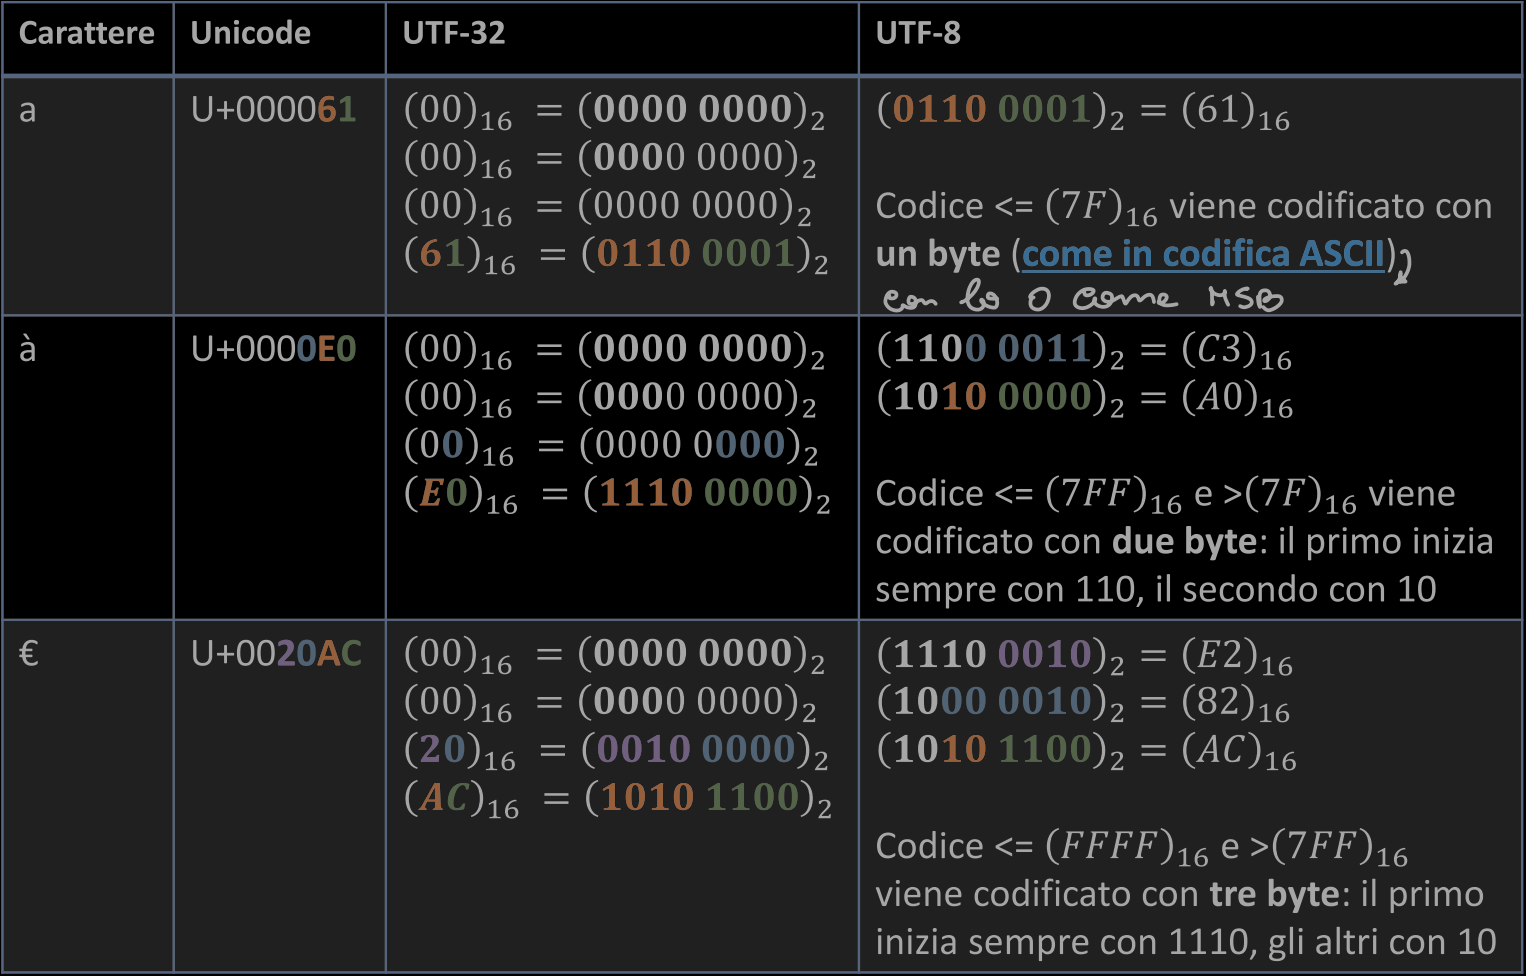
\includegraphics[scale=0.35]{utf32utf8.png}
\end{center}
\section{Reti combinatorie}
\subsection{Reti logiche}
Ridefiniamo in maniera più precisa una \textbf{rete logica}: modello astratto che assume come primitive alcune semplici elaborazioni di segnali binari (gate) e permette di dedurre:
\begin{enumerate}
    \item quale struttura realizza un dato comportamento (\textbf{sintesi})
    \item quale comportamento ha una data struttura (\textbf{analisi})
\end{enumerate}
\begin{center}
    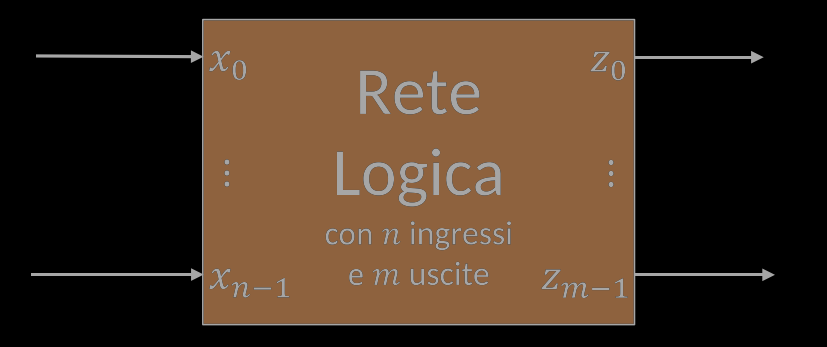
\includegraphics[scale=0.35]{retelog.png}
\end{center}
Si assume come convenzione che gli ingressi siano a sinistra e le uscite a destra e che i nomi dei segnali siano indicati all'interno della rete.
\subsubsection*{Trascodifica BCD/7 Segmenti}
\begin{center}
    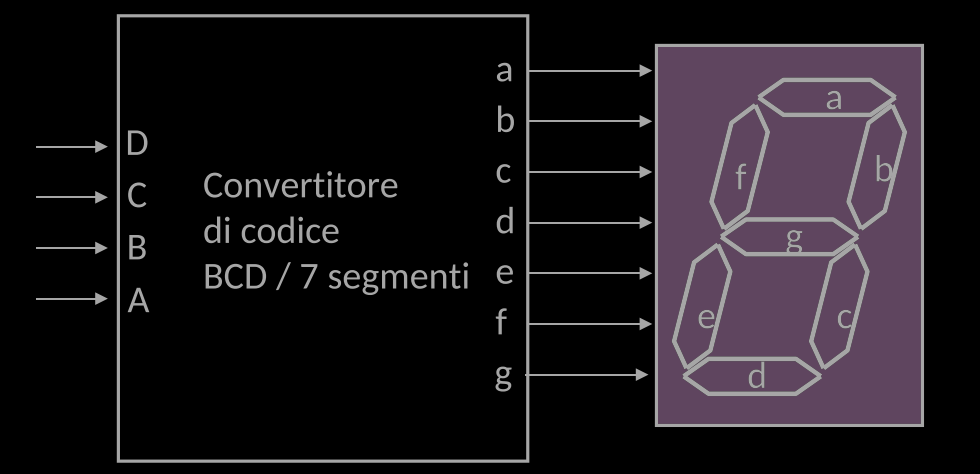
\includegraphics[scale=0.35]{bcd-7.png}
\end{center}
Questo convertitore è un esempio di macchina combinatoria: le 7 uscite (abcdefg) sono univocamente determinate dal valore corrente dei 4 ingressi (DCBA) che codificano un numero senza segno tra 0 e 9.\\
Esempio: $DCBA = 0001 \Rightarrow abcdefg = 1001111$
\subsection{Macchina combinatoria e macchina sequenziale}
In una \textbf{macchina combinatoria} l'uscita dipende esclusivamente dagli ingressi correnti.
\vspace{0.2cm}\\
In una \textbf{macchina sequenziale} l'uscita non è univocamente determinata dagli ingressi correnti, ma dipende anche dalla storia passata (sequenza di ingressi visti in precedenza) e/o dallo scorrere del tempo.
\vspace{0.2cm}\\
Ma come faccio a capire se una rete va realizzata come combinatoria o sequenziale? Se in presenza di una stessa configurazione di ingressi la rete deve fornire 2 o più uscite diverse, allora è una rete sequenziale, altrimenti è una rete combinatoria.
\subsection{Rete logica combinatoria}
In una \textit{rete logica combinatoria} i valori delle variabili di uscita (variabili dipendenti) dipendono solo dai valori contemporanei delle variabili di ingresso (variabili indipendenti).
\subsubsection*{Composizione e decomposizione}
\begin{fbox}
{\textit{La disposizione in serie e/o in parallelo di reti logiche combinatorie è ancora una rete logica combinatoria}}
\end{fbox}
\vspace{0.1cm}\\
Per progettare una rete con $m$ uscite si possono quindi progettare $m$ reti con una sola uscita, operanti in parallelo:
\begin{center}
    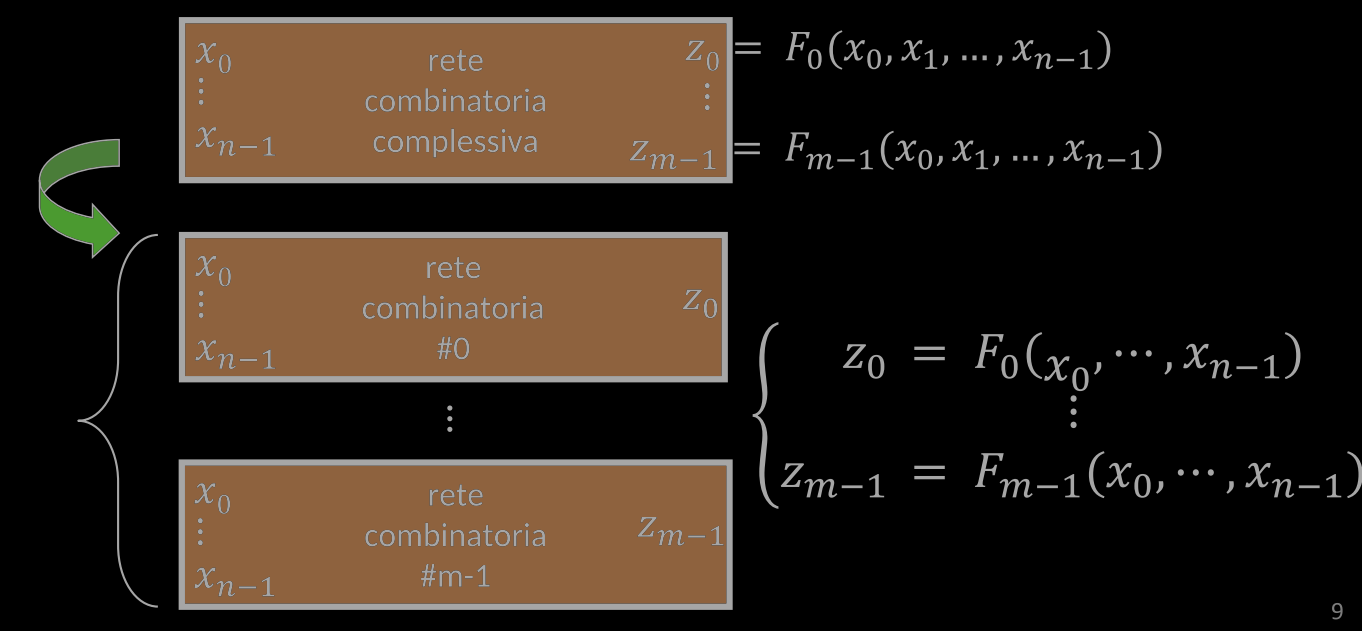
\includegraphics[scale=0.35]{parallel.png}
\end{center}
\subsubsection*{Comportamento e struttura}
\begin{center}
    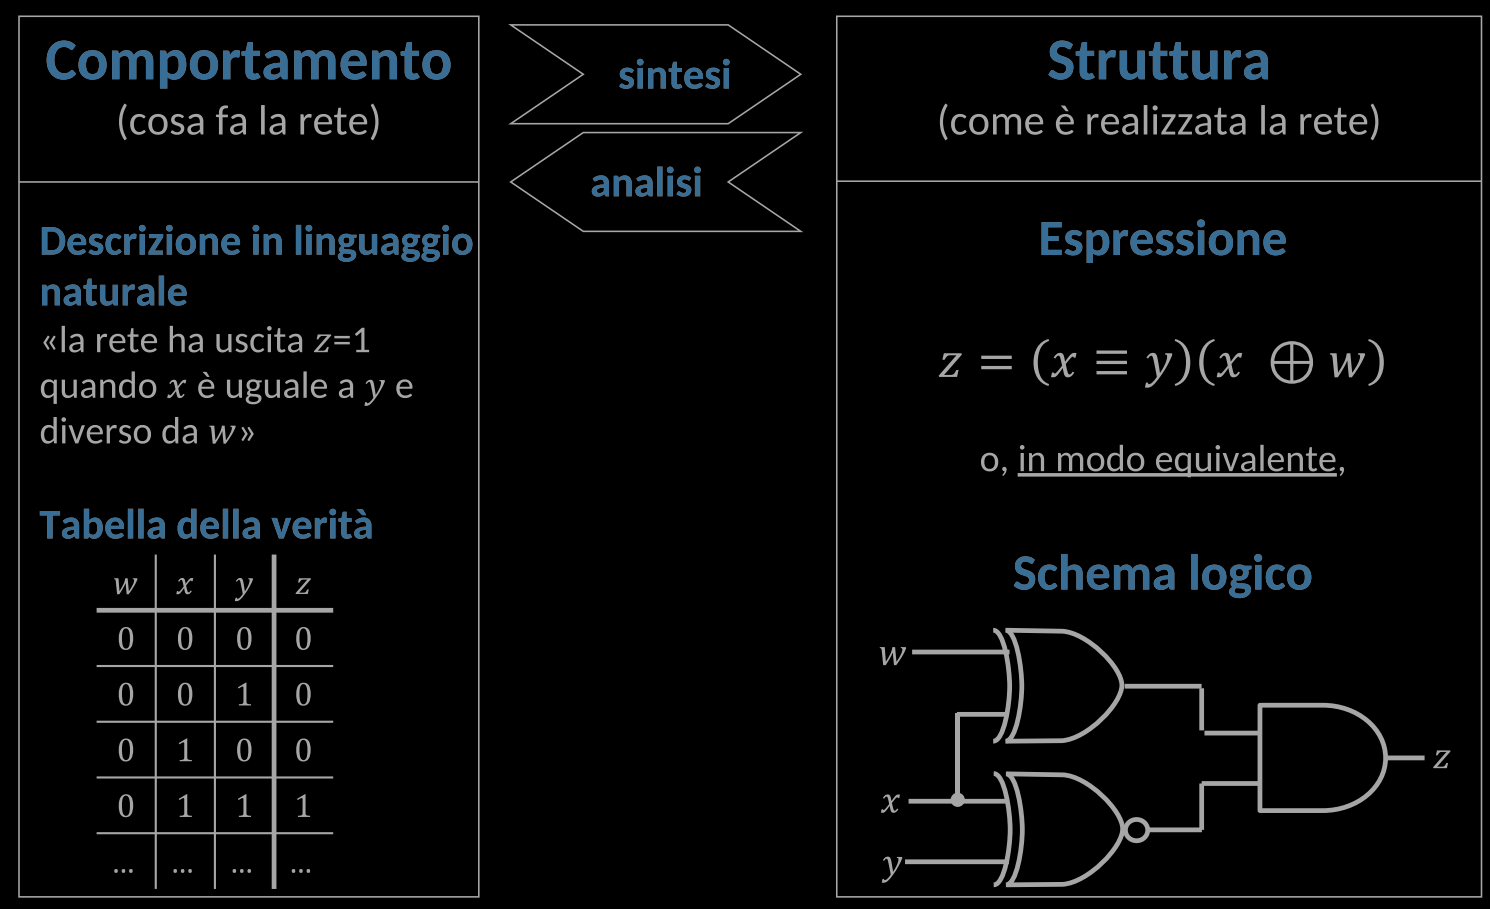
\includegraphics[scale=0.35]{compstr.png}
\end{center}
\subsubsection{Funzioni complete e incomplete}
\textit{Funzione completa} di $n$ variabili binarie $z = F(x_0,x_1,...,x_{n-1})$: per ognuna delle $2^n$ configurazioni degli ingressi è definito il valore dell'uscita $z$ (ne sono esempi il sommatore e il selettore a n vie). 
\vspace{0.2cm}\\
\textit{Funzione incompleta} o non completamente specificata: vi è almeno una configurazione degli ingressi per cui non è specificato il valore dell’uscita, o perché tali configurazioni non possono presentarsi o perché non interessa il valore dell’uscita nel caso in cui si presentino (ne è un esempio il convertitore BCD/7 segmenti).
\subsubsection{Tabella della verità}
La \textit{tabella della verità} descrive univocamente il comportamento di una rete combinatoria a $n$ ingressi (ovvero di una funzione $F$ di $n$ variabili binarie $x_0,x_1,...,x_{n-1}$).
\vspace{0.1cm}\\
Nel caso di funzioni non specificate si possono avere
\begin{itemize}
    \item meno righe, evitando di riportare le configurazioni di input che non possono presentarsi
    \item il simbolo \textit{don't care} nelle uscite al posto di 0 e 1 a indicare una condizione di indifferenza, cioè il valore di quell'uscita non interessa al fine del progetto
\end{itemize}
\textbf{N.B.} il \textit{don't care} non vuol dire che quell'uscita non ha né valore 1 né valore 0.
\subsubsection*{Convertitore BCD/7 Segmenti}
\begin{center}
   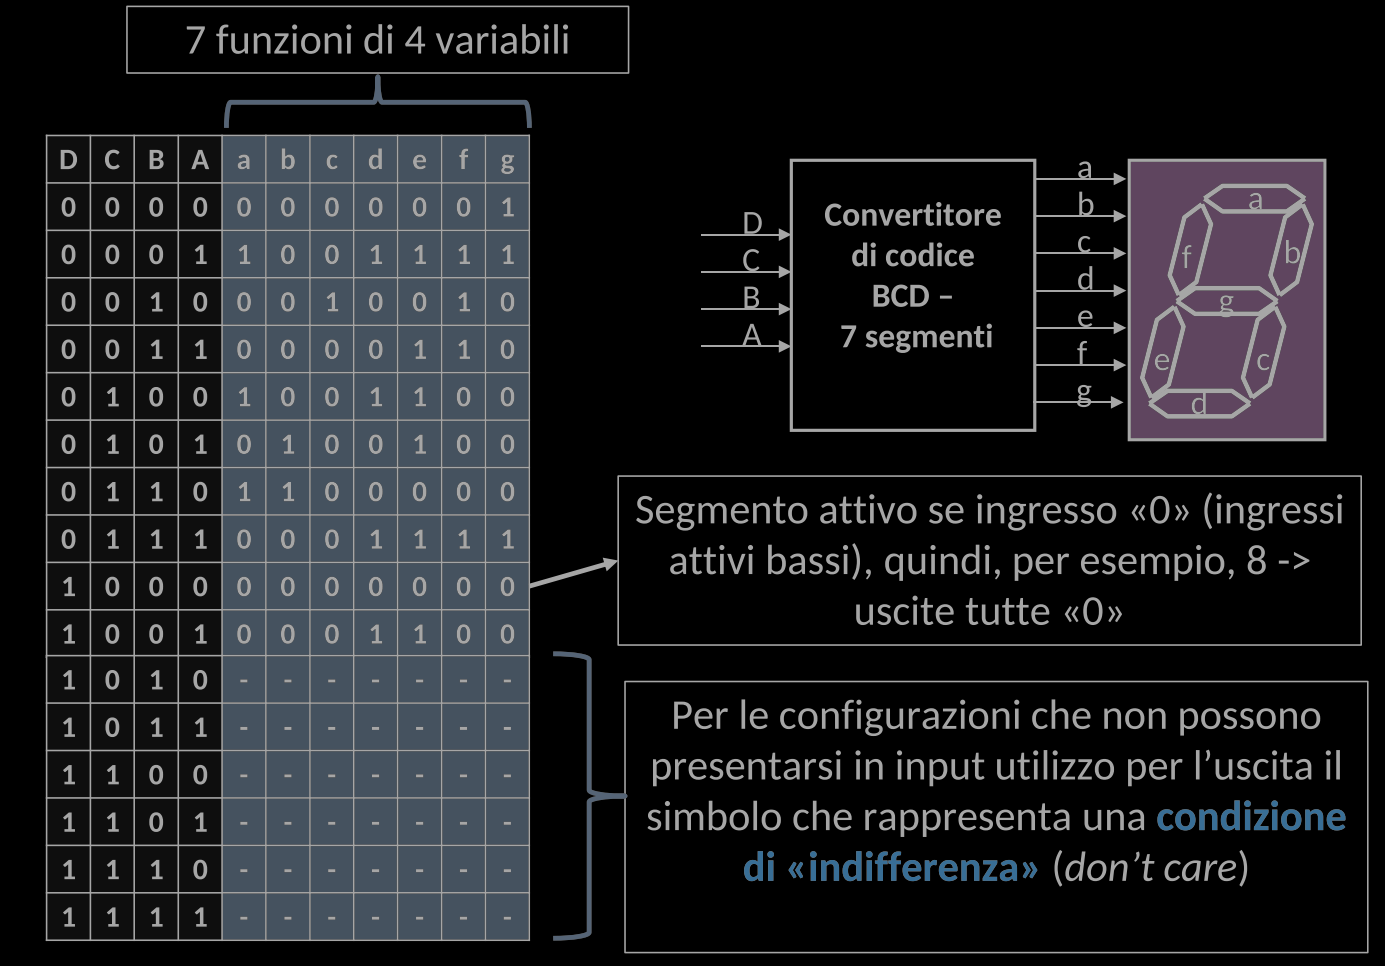
\includegraphics[scale=0.34]{conv7.png}
\end{center}
\subsubsection{Funzioni complete di n variabili}
Il numero di distinte funzioni esistenti di $n$ variabili binarie è
$$  \Phi(n) = 2^{2^n} $$
Siccome il numero complessivo di funzioni aumenta esponenzialmente con $n$ (e anche di molto, per $n = 4$ si hanno 65536 funzioni possibili) i costruttori non forniscono la realizzazione ad hoc di ogni funzione ma è il progettista che deve realizzarle tramite
opportuna composizione di gate elementari disponibili in forma di circuiti integrati.
\subsection{Algebre binarie}
Un'\textit{Algebra Binaria} è un sistema matematico formato da un insieme di operatori definiti assiomaticamente e atti a descrivere con un'espressione ogni possibile funzione di variabile binaria.
\begin{center}
    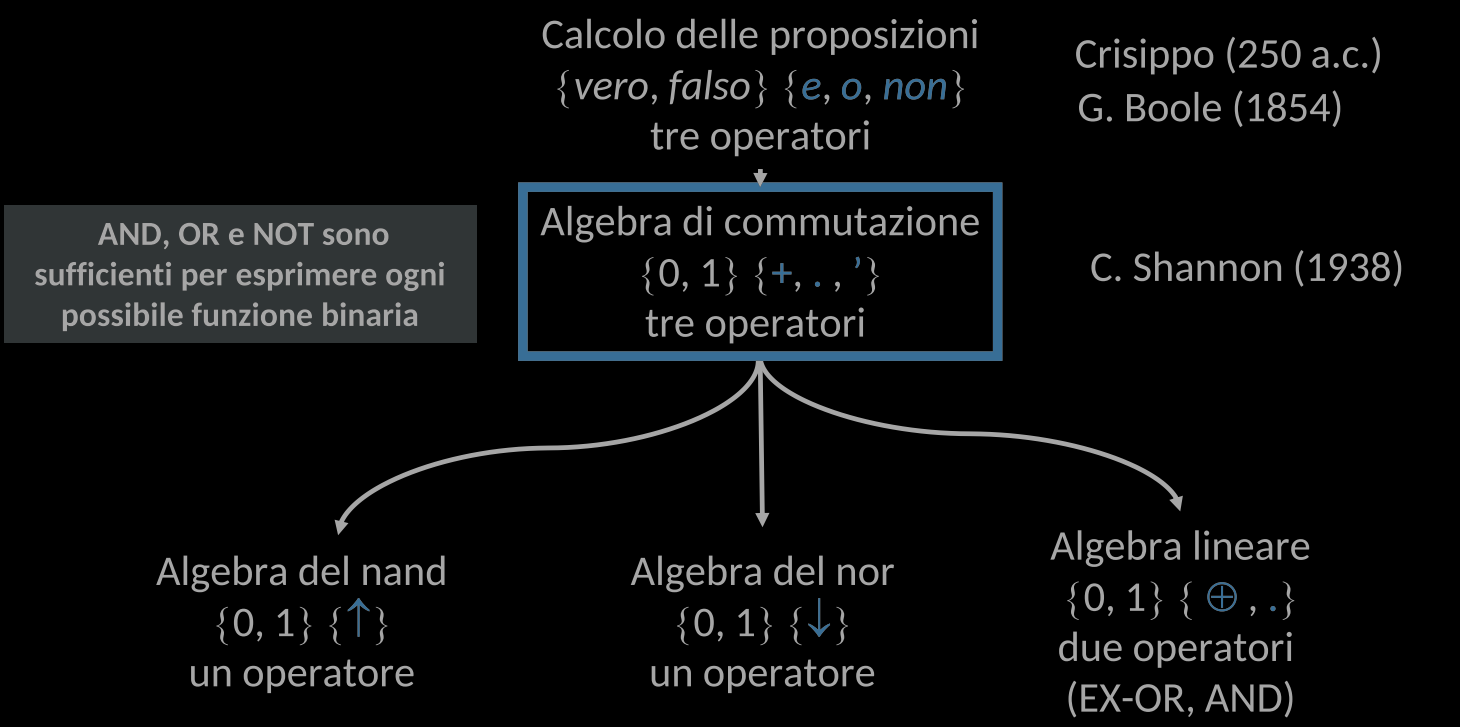
\includegraphics[scale=0.33]{algmap.png}
\end{center}
\subsubsection{Algebra di commutazione}
Un' \textit{algebra di commutazione} è un'algebra binaria definita da:
\begin{enumerate}
    \item un insieme di simboli $B = \{ 0,1 \}$
    \item un insieme di operazioni $O = \{ +,.,'\}$, ovvero \underline{somma logica}, \underline{prodotto logico} e \underline{complementazione}
    \item un insieme di postulati $P$:
    \begin{align*}
        &\text{OR} && &\text{AND} && &\text{NOT}\\
        &0+0 = 0 && &0.0=0 && &0'=1\\
        &1+0=1 && &1.0=0 && &1'=0\\
        &0+1=1 && &0.1=0\\
        &1+1=1 && &1.1=1\\
    \end{align*}
\end{enumerate}
\subsubsection{Definizione di espressione}
Nelle espressioni che trattiamo noi vi sono due \textbf{costanti}, che sono 0 e 1, e delle \textbf{variabili} letterali che possono assumere il valore 0 o 1.\\
Un'\textit{espressione} è definita come una stringa di costanti, variabili, operatori e parentesi, formate in accordo alle seguenti regole:
\begin{enumerate}
    \item 0 e 1 sono espressioni
    \item una variabile è una espressione
    \item se A è un'espressione lo è anche $(A')$
    \item se A, B sono espressioni, lo sono anche $(A+B)$ e $(A \cdot B)$
\end{enumerate}
\textbf{N.B.} La notazione AB indica A.B.
\subsection{Espressioni e schemi logici}
\textit{Schema logico}: Descrizione grafica di una struttura formata da simboli di gate e da collegamenti tra le loro linee di ingresso e di uscita.
\vspace{0.2cm}\\
\textbf{Relazione I:} Ogni struttura formata da gate connessi in serie e/o in parallelo è descritta da \underline{una sola espressione}.
\begin{center}
    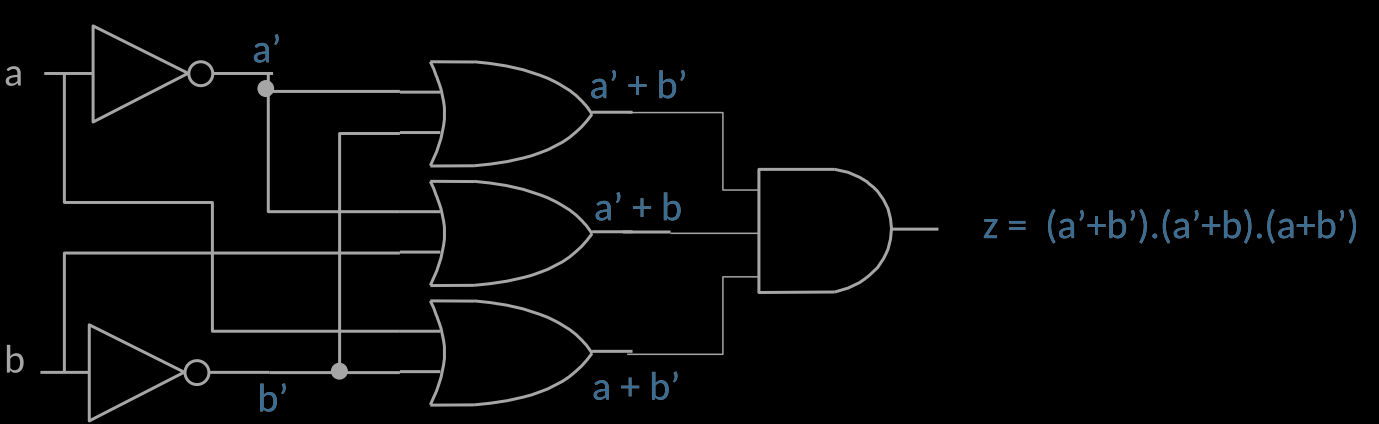
\includegraphics[scale=0.42]{imesp.png}
\end{center}
\textbf{Relazione II:} Ogni espressione descrive una sola struttura formata da gate connessi in serie e/o in parallelo.
\vspace{0.2cm}\\
Per individuare lo schema descritto da una espressione:
\begin{enumerate}
    \item si parte dalle parentesi più interne e si traccia il simbolo del gate corrispondente all'operazione, collegandone gli ingressi ai segnali esterni;
    \item si procede in modo analogo con le altre coppie di parentesi, considerando via via come ingressi dei nuovi gate anche le uscite di quelli già tracciati.
\end{enumerate}
Per esempio lo schema logico dell'espressione $a+(b.c)$ è
\begin{center}
    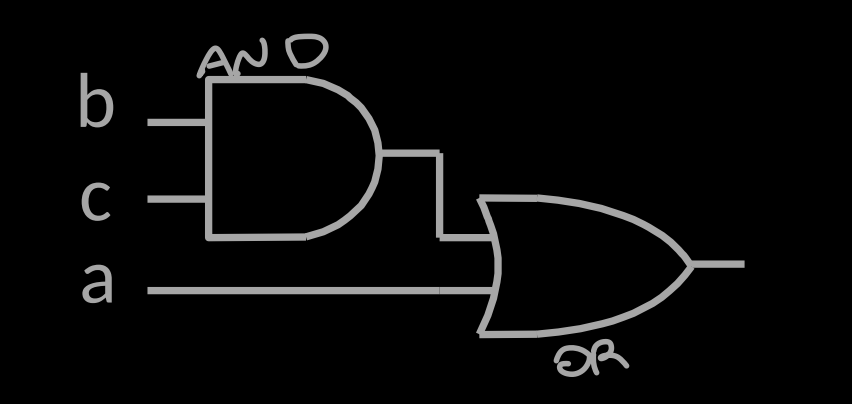
\includegraphics[scale=0.35]{esp1}
\end{center}
\subsubsection*{Altri esempi}
\begin{center}
    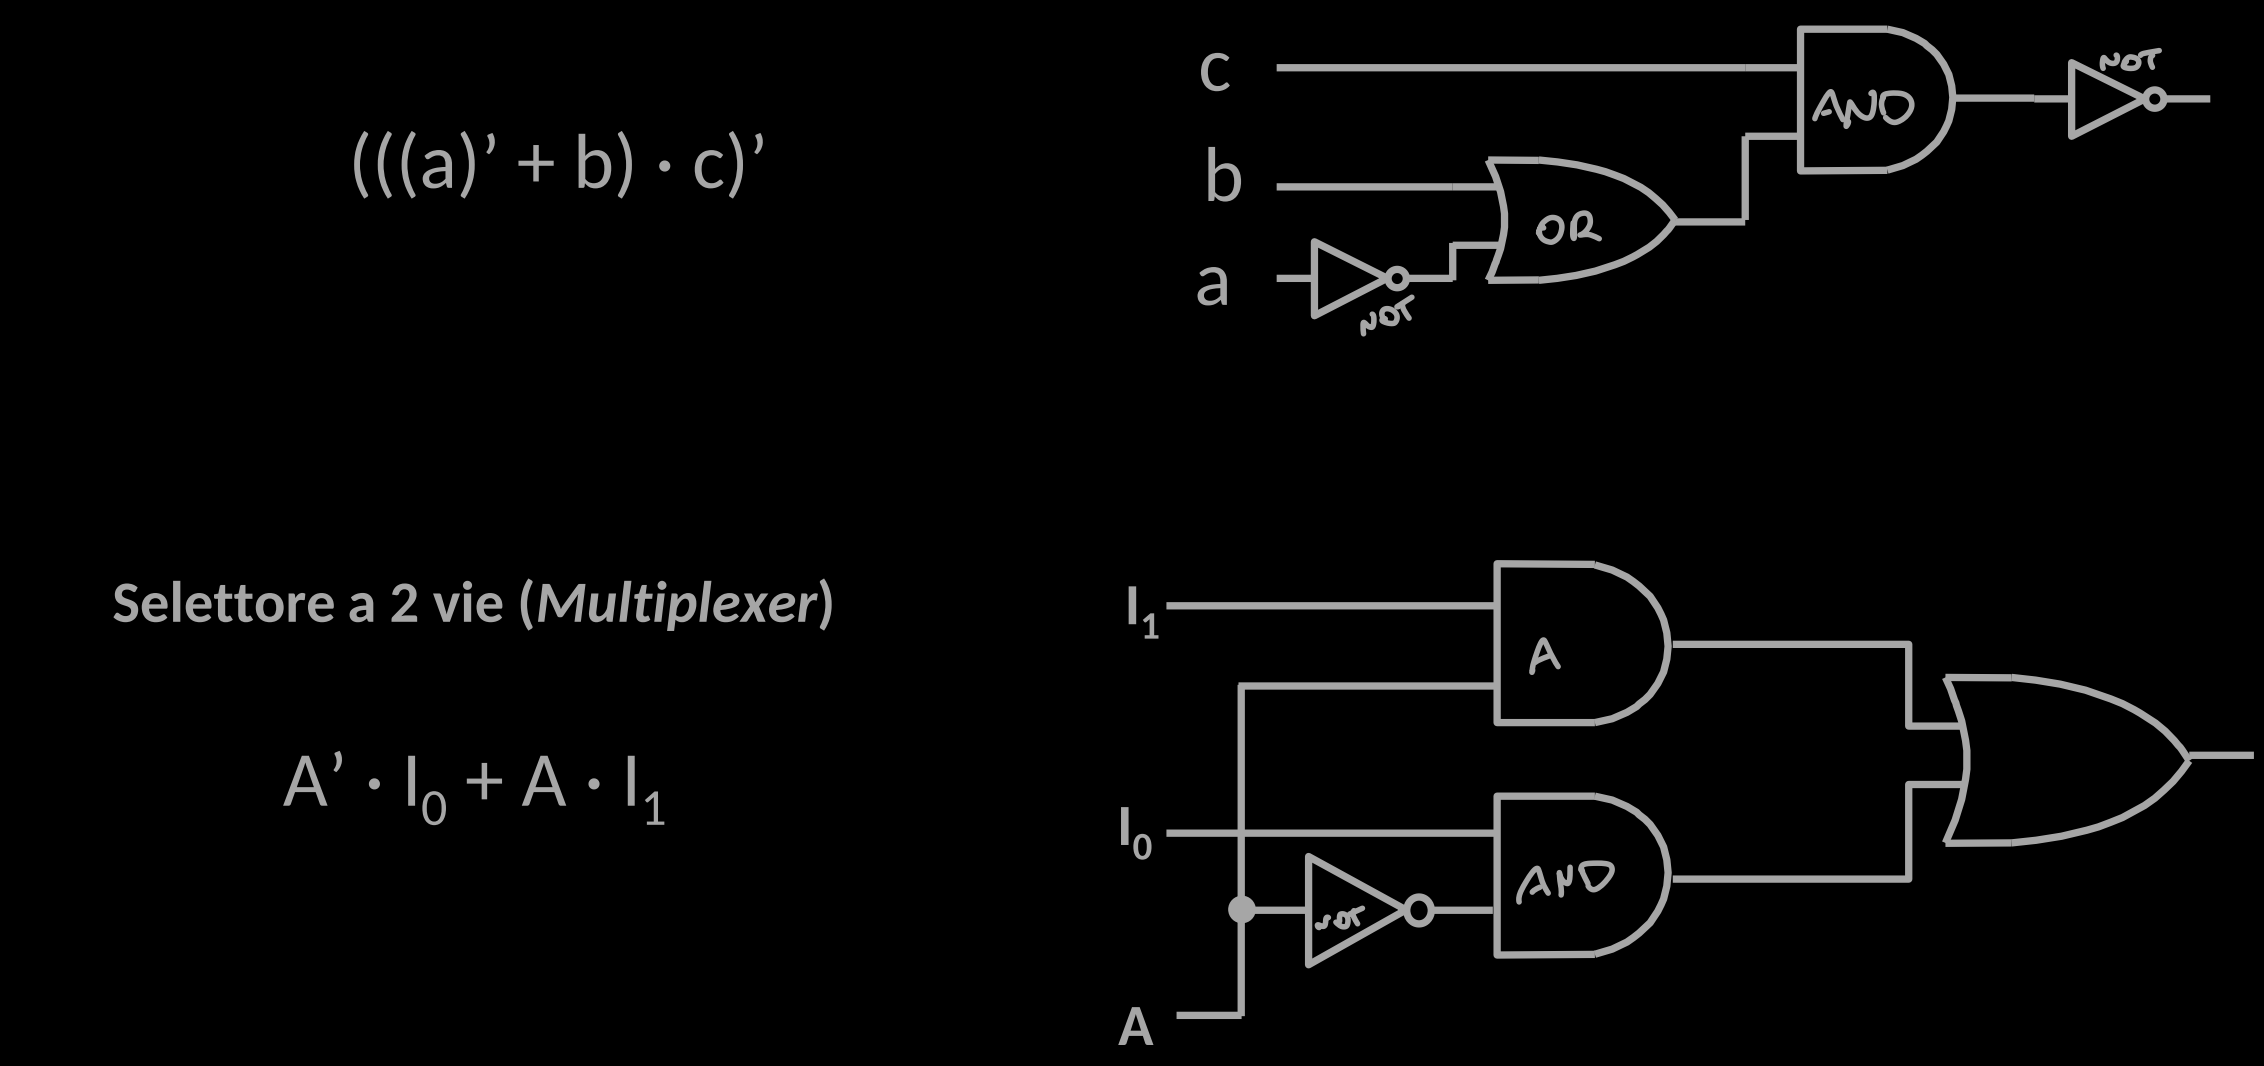
\includegraphics[scale=0.3]{esp2}
\end{center}
\textbf{N.B.} Non ci possono essere segnali in retroazione in una rete combinatoria.
\par\noindent\rule{\textwidth}{0.4pt}
Da ciò che abbiamo appena visto si evince che esiste una relazione biunivoca tra schemi ed espressioni. Quindi per esprimere la struttura con cui si realizza una funzione si può usare o uno schema o un'espressione, ma è preferibile utilizzare l'espressione perché più compatta. 
\subsubsection{Valutazione di un'espressione}
Per valutare un'espressione:
\begin{itemize}
    \item si sostituisce ad ogni variabile il valore che ha nella n-upla
    \item partendo dalle parentesi più interne, si sostituisce ogni operazione con il suo risultato fino ad ottenere o la costante 0 o la costante 1
\end{itemize}
\textbf{N.B.} Una espressione di $n$ variabili può essere valutata in $2^n$ modi diversi, che corrispondono alle $n$ configurazioni binarie dei suoi ingressi. Valutando una espressione di $n$ variabili per tutte le possibili $2^n$ configurazioni, ottengo la tabella della verità, ovvero il comportamento della rete combinatoria che ha quella struttura.
\subsubsection{Da espressioni a Tabella della verità}
\textbf{Relazione III:} Ogni espressione descrive una e una sola tabella della verità completamente specificata.
\vspace{0.3cm}\\
Proviamo a scrivere la tabella della verità della funzione $E(a,b,c) = a +(b.c)$
\begin{center}
    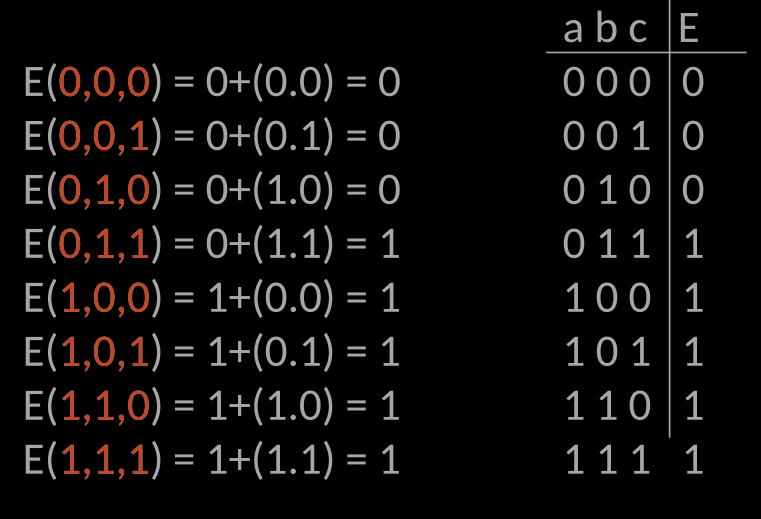
\includegraphics[scale=0.44]{tdv1.png}
\end{center}
\subsection{Da Tabella della verità a espressioni}
\textbf{Relazione VI:} Una funzione può essere descritta da una molteplicità di espressioni.
\vspace{0.2cm}\\
Uno dei metodi più semplici per passare da una tabella della verità a una delle possibili espressioni riguarda l'utilizzo di \underline{espressioni canoniche}.
\begin{center}
    \textbf{Espressione canonica SP (Somma di Prodotti) o \textit{I forma canonica}}
\end{center}
Ogni funzione di $n$ variabili è descritta da una somma di tanti prodotti logici quante sono le configurazioni per cui vale 1. In ciascun prodotto, o \underline{mintermine}, appare ogni variabile, in forma vera se nella configurazione corrispondente vale 1, in forma negata se vale 0.
\vspace{0.1cm}\\
In pratica si scrivono tutti i vari mintermini, riferiti a ogni uscita uguale a 1, come prodotto logico tra le variabili, che vengono negate se valgono 0, e si mettono in OR tra di loro, cioè in somma logica, ottenendo così la prima forma canonica.
\begin{center}
    \textbf{Espressione canonica PS (Prodotto di Somme) o  \textit{II forma canonica}}
\end{center}
Ogni funzione di $n$ variabili è descritta da un prodotto di tante somme logiche quante sono le configurazioni per cui vale 0. In ciascuna somma, o \underline{maxtermine}, appare ogni variabile, in forma vera se nella configurazione corrispondente vale 0, in forma negata se vale 1.
\vspace{0.1cm}\\
In questo caso invece si scrivono i mextermini, riferiti a ogni uscita uguale a 0, come somma logica delle variabili, che vengono negate se valgono 1, e si mettono in AND tra loro, cioè con un prodotto logico, ottenendo la seconda forma canonica.
\subsubsection{Notazione simbolica}
Prendiamo in esempio la tabella della verità del Full Adder:
\begin{center}
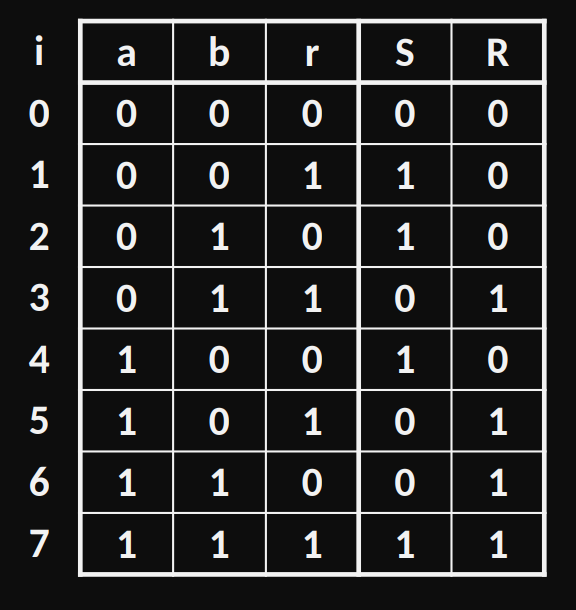
\includegraphics[scale=0.27]{fulladderTdv.png}
\end{center}
\begin{align*}
    &S(a,b,r) = \sum_{i=0}^3 m_i(1,2,4,7) && &R(a,b,r) = \sum_{i=0}^3 m_i (3,5,6,7)\\
    &S(a,b,r) = \prod_{i=0}^3 M_i (0,3,5,6) && &R(a,b,r) = \prod_{i=0}^3 M_i(0,1,2,4)
\end{align*}
$m_i :=$ mintermine di $n$ bit che assume il valore 1 solo per la n-pla di valori delle variabili corrispondenti all'indice $i$;\\
$M_i :=$ maxtermine di $n$ bit che assume il valore 0 solo per la n-pla di valori delle variabili corrispondente all'indice $i$.
\textbf{N.B.} Mintermini e maxtermini sono complementari: una configurazione deve essere o un mintermine o un maxtermine
\subsubsection{Equivalenza tra espressioni}
Due espressioni si dicono \textit{equivalenti} se e solo se descrivono la stessa funzione o tabella della verità.\\
Ne sono un esempio le due espressioni canoniche nella forma PS e SP.
\vspace{0.2cm}\\
Espressioni equivalenti possono avere complessità algebrica differente, a cui di conseguenza corrispondono schemi logici di \textbf{complessità differente}.
\vspace{0.1cm}\\
Esempio: funzione $U$ di 3 variabili $a,b,c$ con 6 mintermini e 2 maxtermini:
$$ U(a,b,c) = \sum_{i=0}^3 m_i(0,1,2,3,4,5)  = \prod_{i=0}^3 M_i(6,7) $$
La forma canonica SP richiede 6 AND e 1 OR, mentre la forma PS 2 OR e 1 AND; rappresentano entrambe la stessa funzione ma la seconda è estremamente meno complessa:
\begin{center}
    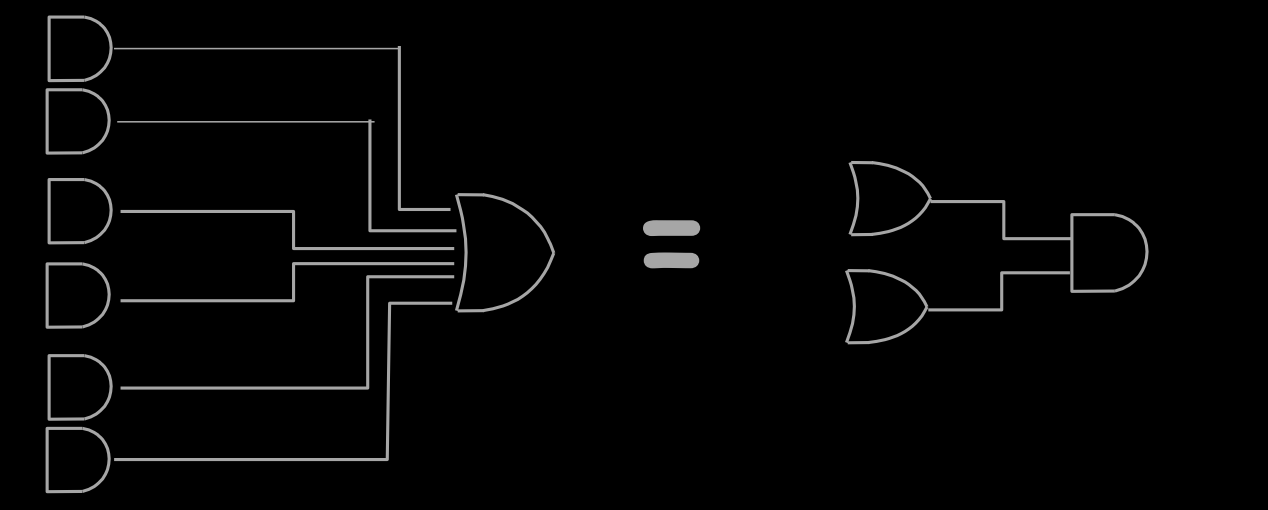
\includegraphics[scale=0.3]{es3}
\end{center}
\subsubsection{Espressioni di funzioni incomplete}
Espressioni che forniscono eguale valutazione limitatamente al dominio di una funzione incompleta sono dette equivalenti.
Esempio: a seconda del valore assegnato alle configurazioni non utilizzate dalla funzione che realizza un Encoder a 3 ingressi, ottengo una famiglia di espressioni diverse tra loro equivalenti.
\begin{center}
    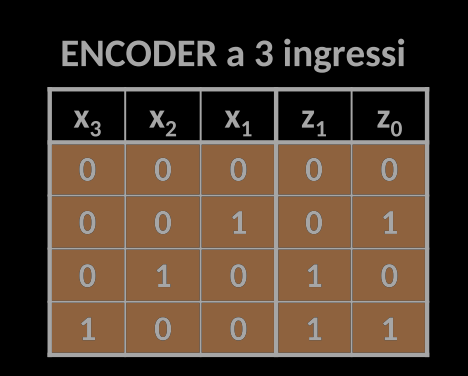
\includegraphics[scale=0.5]{enc3ing.png}
\end{center}
\subsection{Sintesi di reti combinatorie}
Per realizzare la sintesi di una data funzione si può scegliere un'espressione tra tutte le possibili (vedi le espressioni canoniche) e operare nel dominio delle espressioni per ridurne la complessità mediante l'utilizzo delle equivalenze notevoli dell'algebra di commutazione.
\subsubsection{Equivalenze notevoli}
Proprietà della somma e del prodotto logico:
\begin{itemize}
    \item [$\blacktriangleright$] \textit{E1) commutativa} 
    \begin{align*}
        x+y &= y+x\\
        x \cdot y  &= y \cdot x
    \end{align*}
    \item [$\blacktriangleright$] \textit{E2) associativa}
    \begin{align*}
        (x+y)+z &= x+y+z\\
        (x \cdot y) \cdot z &= x \cdot y \cdot z
    \end{align*}
    \item [$\blacktriangleright$] \textit{E3) distributiva}
    \begin{align*}
        (x \cdot y) + (x \cdot z) &= x \cdot (y + z)\\
        (x+y)\cdot (x+z) &= x + (y \cdot z)
    \end{align*}
    \item [$\blacktriangleright$] \textit{E4) idempotenza}
    \begin{align*}
        x + x &= x\\
        x \cdot x &= x
    \end{align*}
    \item [$\blacktriangleright$] \textit{E5) identità}
    \begin{align*}
        x+0 &= x\\
        x \cdot 1 &= x
    \end{align*}
    \item [$\blacktriangleright$] \textit{E6) limite}
    \begin{align*}
        x+1 &= 1\\
        x \cdot 0 &= 0
    \end{align*}
\end{itemize}
Proprietà della complementazione:
\begin{itemize}
    \item [$\blacktriangleright$] \textit{E7) involuzione}
    $$ (x')' = x $$
    \item [$\blacktriangleright$] \textit{E8) limitazione}
    \begin{align*}
        x + x' &= 1\\
        x \cdot x' &= 0
    \end{align*}
    \item [$\blacktriangleright$] \textit{E9) combinazione}
    \begin{align*}
        &xy + xy' = x\\
        &(x+y)\cdot (x+y') = x
    \end{align*}
    \item [$\blacktriangleright$] \textit{E10) I e II legge di De Morgan}
    $$ (x+y)'= x'\cdot y' $$
    $$ (x \cdot y)' = x'+ y' $$
\end{itemize}
Le leggi di De Morgan sono molto utili per determinare espressioni equivalenti utilizzando gate logici diversi, come NOR/NAND al posto di AND/OR.\\
Equivalentemente, le leggi di De Morgan asseriscono che:
\begin{align*}
    x +y &= ((x+y)')'\\
    x+y &= (x' \cdot y')'
\end{align*}
\begin{itemize}
    \item [$\blacktriangleright$] \textit{E11) consenso}
    \begin{align*}
        xy+x'z+yz &= xy + x'z\\
        (x+y)\cdot (x'+z)\cdot (y+z) &= (x+y)\cdot (x'+z)
    \end{align*}
\end{itemize}
\subsubsection{Manipolazione algebrica di espressioni}
Lo schema circuitale relativo all'espressione canonica SP del "riporto" (R) di un Full Adder richiede 4 AND a 3 ingressi ciascuno e, in cascata, 1 OR a 4 ingressi e 3 NOT per avere gli ingressi in forma vera e negata.
$$
    R = a'br+ab'r+abr'+abr
$$
\begin{center}
    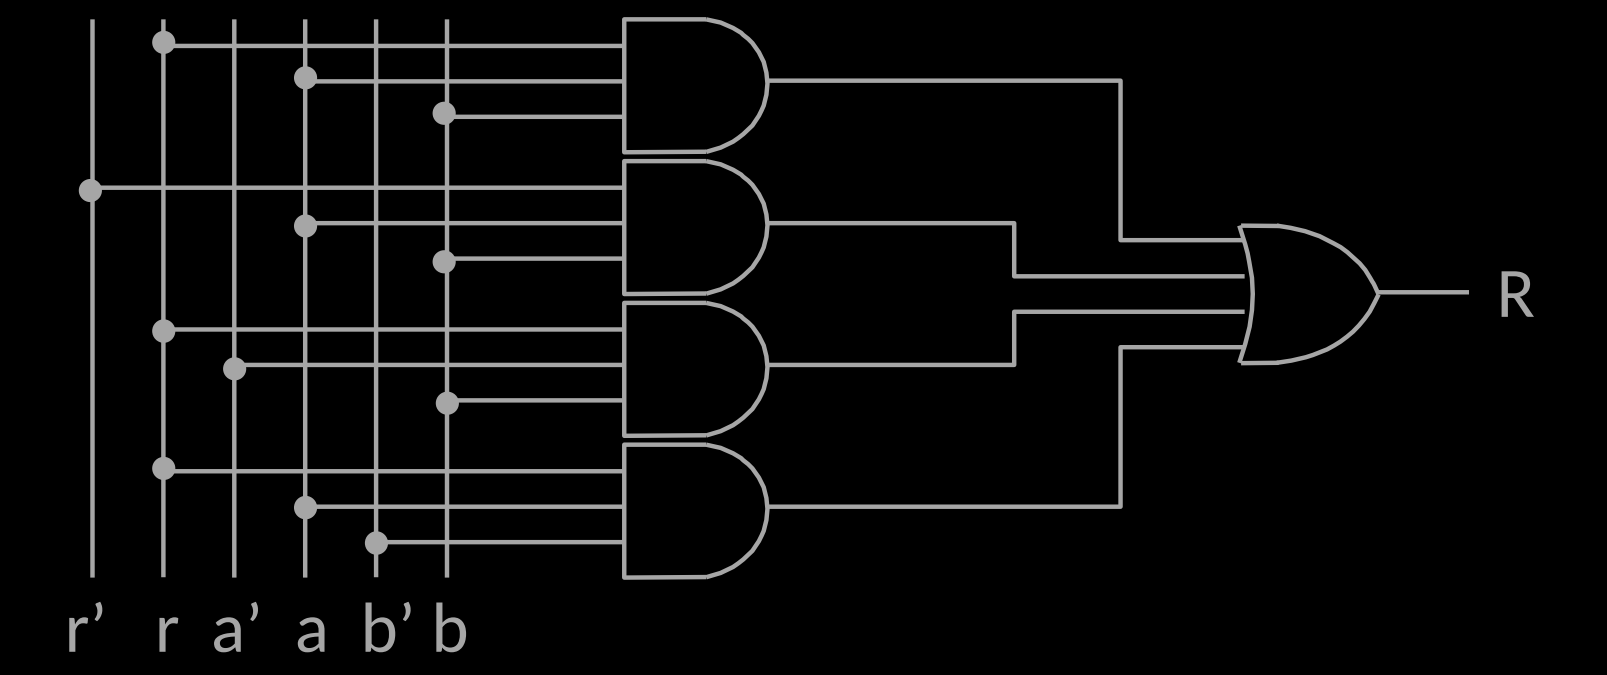
\includegraphics[scale=0.35]{FullAdder1.png}
\end{center}
È possibile ottenere un'espressione più semplice, ecco un modo:
$$ R = a'br+ab'r+\underbrace{abr'+abr}_{\text{distributiva}} $$
$$= a'br+ab'r+ ab\underbrace{(r'+r)}_{\text{limitazione}} = $$
$$= a'br+ab'r+ \underbrace{ab1}_{\text{identità}} $$
$$ = a'br+ab'r+ ab $$
\subsubsection{Il problema della sintesi}
La \textit{sintesi} consiste nell'individuare l'espressione che fornisce lo schema migliore per la realizzazione della funzione assegnata. Il problema è che migliore può essere definito con criteri a volte opposti tra loro: rapidità di progetto, massima velocità, massima flessibilità, minima complessità.
\vspace{0.2cm}\\
Di seguito un piccolo schema che spiega un po' le differenze che ci possono essere tra progetti in base alle finalità degli stessi:
\begin{center}
    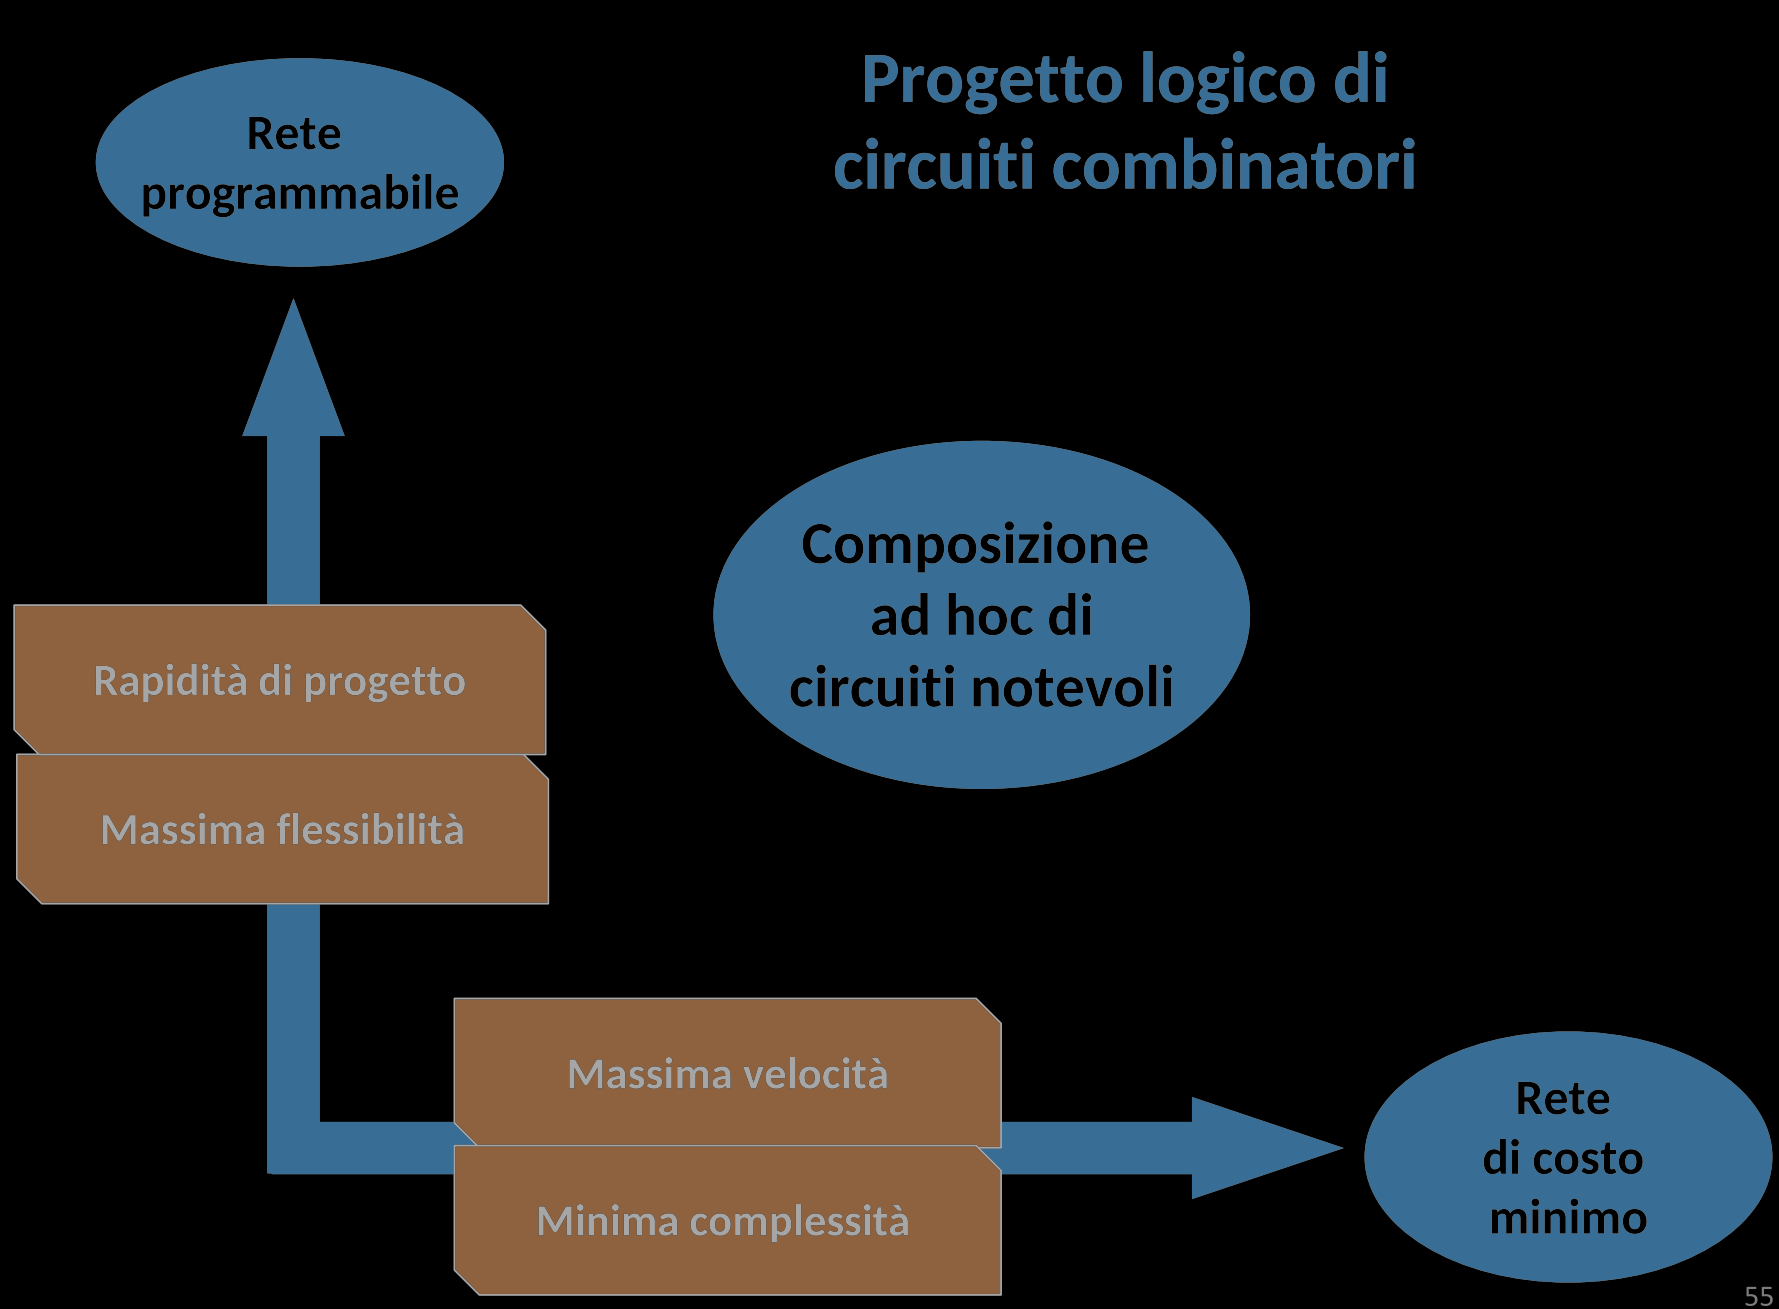
\includegraphics[scale=0.3]{proglog.png}
\end{center}
\section{Reti di costo minimo}
\subsection{Introduzione}
\subsubsection{Ritardi e velocità}
Abbiamo già visto che la differenza tra la tabella della verità e un gate reale è il ritardo di propagazione (Quando cambia un ingresso di un gate, l'uscita non cambia istantaneamente, ma dopo un tempo $\tau_p$ che dipende dalla tecnologia utilizzata). $\tau_p$ è diverso da gate a gate, ma in prima approssimazione assumeremo che ogni gate introduca un ritardo uguale. Quindi, il ritardo complessivo introdotto da una rete combinatoria è dato, nel caso peggiore, dal numero di gate sul percorso più lungo tra ingressi e uscite; questo è il ritardo che noi assegneremo alla rete complessiva.
\subsubsection{Complessità e velocità}
Per confrontare \textbf{complessità} e \textbf{velocità di risposta} di reti combinatorie equivalenti useremo 3 indicatori:
\begin{itemize}
    \item $N_{gate}=$ numero di gate; maggiore è $N_{gate}$ maggiore è la complessità
    \item $N_{conn}=$ numero di connessioni (ovvero ingressi); maggiore è $N_{conn}$ maggiore è la complessità
    \item $N_{casc}=$ massimo numero di gate disposti in cascata, ovvero in serie tra ingresi e uscita; minore è $N_{casc}$ maggiore è la velocità.
\end{itemize}
\begin{center}
    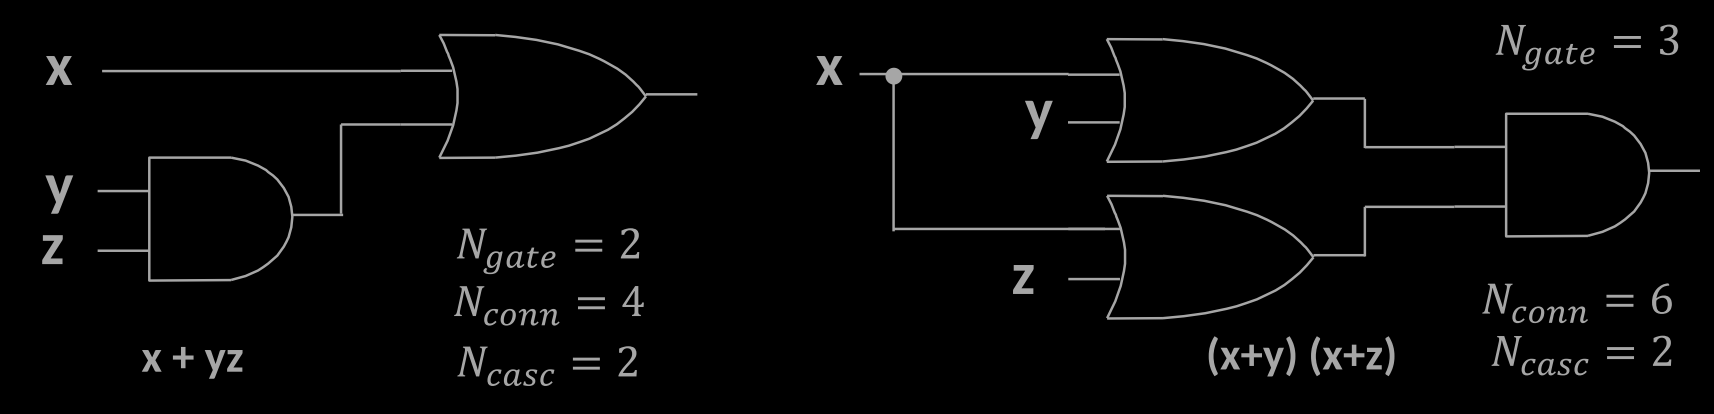
\includegraphics[scale=0.38]{escompl.png}
\end{center}
Le due reti sono equivalenti (proprietà distributiva), hanno la stessa velocità di elaborazione, ma la rete di sinistra è meno complessa.
\subsection{Come si definisce una rete di costo minimo}
Per definire una rete di costo minimo bisogna che siano soddisfatte due ipotesi:
\begin{itemize}
    \item gli ingressi devono essere disponibili in forma vera e negata
    \item il fan-in dei gate deve essere grande quanto serve
\end{itemize}
Definizione di una \textit{rete combinatoria di costo minimo:}
\vspace{0.1cm}\\
Schema logico ed espressione (minima) che realizzano una funzione qualsiasi con:
\begin{enumerate}
    \item non più di 2 gate in cascata tra ingressi e uscita;
    \item minimo numero di gate;
    \item minimo numero di ingressi per gate.
\end{enumerate}
\textbf{N.B.} Il numero di gate e/o di connessioni della rete di costo minimo di tipo SP è in generale diverso da quello della rete di costo minimo di tipo PS.\\
\textbf{N.B.2} È possibile che più espressioni dello stesso tipo (PS o SP) siano minime (abbiamo quindi eguali valori di $N_{gate}$ e $N_{con}$; $N_{casc}$ è eguale e sempre minore o uguale a 2.
\subsubsection{Implicanti e implicanti primi}
\textbf{Implicante:} termine prodotto di $n$ o meno variabili che assume il valore 1 solo per configurazioni in cui la funzione vale 1 o indifferenza.
\vspace{0.2cm}\\
Per esempio per una funzione $z$ di questo tipo
\begin{center}
    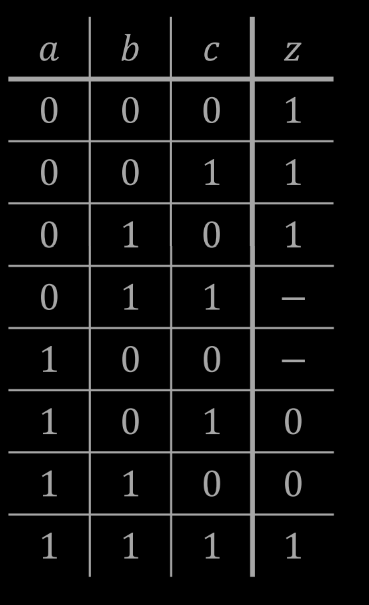
\includegraphics[scale=0.45]{zfun.png}
\end{center}
gli implicanti sono 
\begin{center}
    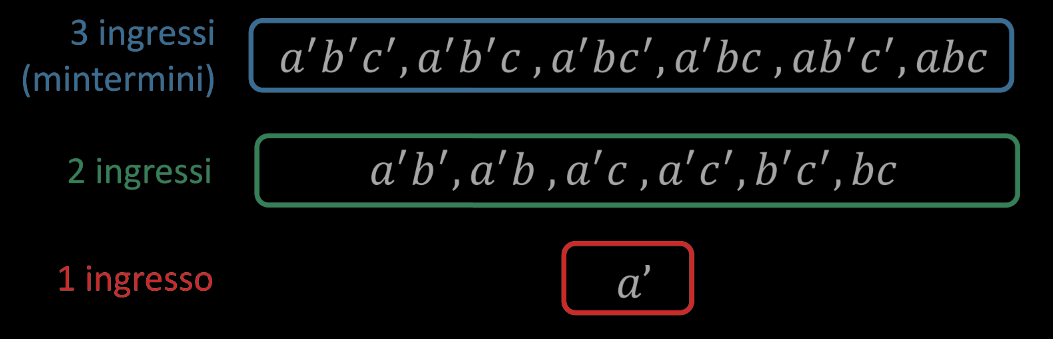
\includegraphics[scale=0.4]{impZ.png}
\end{center}
\textbf{Implicante primo:} implicante che cessa di essere tale rimuovendo un suo letterale
\begin{center}
    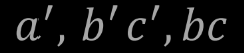
\includegraphics[scale=0.45]{imp1Z.png}
\end{center}
\textbf{N.B.} Si può avere un implicante a 0 ingressi in casi degeneri, come il caso della funzione che da in uscita sempre 1.
\vspace{0.3cm}\\
\textbf{Implicante primo essenziale:} implicante che è \textbf{l'unico} ad assumere il valore 1 per alcune configurazioni delle variabili di ingresso in cui la funzione assume il valore 1 (cioè non vi sono altri implicanti primi che possono coprire uno o più "uni" della funzione).
\begin{center}
    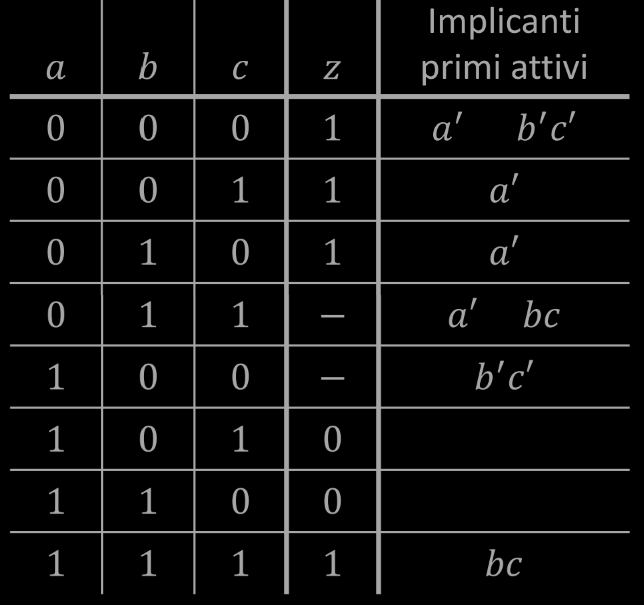
\includegraphics[scale=0.45]{imp1att.png}
\end{center}
$a'$ è l'unico implicante primo a valere 1 per la configurazione di ingresso 001 e 010 quindi \textbf{è essenziale}; $bc$ è l'unico ad assumere il valore 1 per 111, quindi è essenziale; $b'c'$ assume valore 1 per 000, dove anche $a'$ vale 1 quindi non è essenziale.
\vspace{0.2cm}\\
\textbf{L'espressione minima SP è la somma di implicanti primi essenziali}
$$ F(a, b,c) = a'+bc $$
\subsubsection{Implicati e implicati primi}
\textbf{Implicato:} termine somma di $n$ o meno variabili che assume il valore 0 solo per configurazioni in cui la funzione vale 0 o indifferenza.
$$ a+b'+c', a'+b+c, a'+b+c', a'+b'+c, a'+c, a'+b $$
\textbf{Implicato primo:} implicato che cessa di essere tale rimuovendo un suo letterale.
$$ a+b'+c', a'+c, a'+b $$
\textbf{Implicato primo essenziale:} unico implicato ad assumere il valore 0 per alcune configurazioni delle variabili di ingresso in cui la funzione assume il valore 0 (cioè non vi sono altri implicati primi che possono coprire uno o più zeri della funzione).
$$ a'+c, a'+b $$
L'espressione minima PS è il prodotto di implicati minimi essenziali.
$$ F = (a'+c)(a'+b) $$
\subsection{Mappe di Karnaugh}
Una \textit{mappa di Karnaugh} è una rappresentazione bidimensionale della tabella della verità di una funzione di 2,3,4 variabili, i cui valori sono elencati sui bordi in maniera tale che due configurazioni consecutive differiscano per il valore di un solo bit (codice di Gray).
\vspace{0.1cm}\\
Per esempio, nel caso della tabella della verità del Full Adder la mappa di Karnaugh corrispondente è la seguente:
\begin{center}
    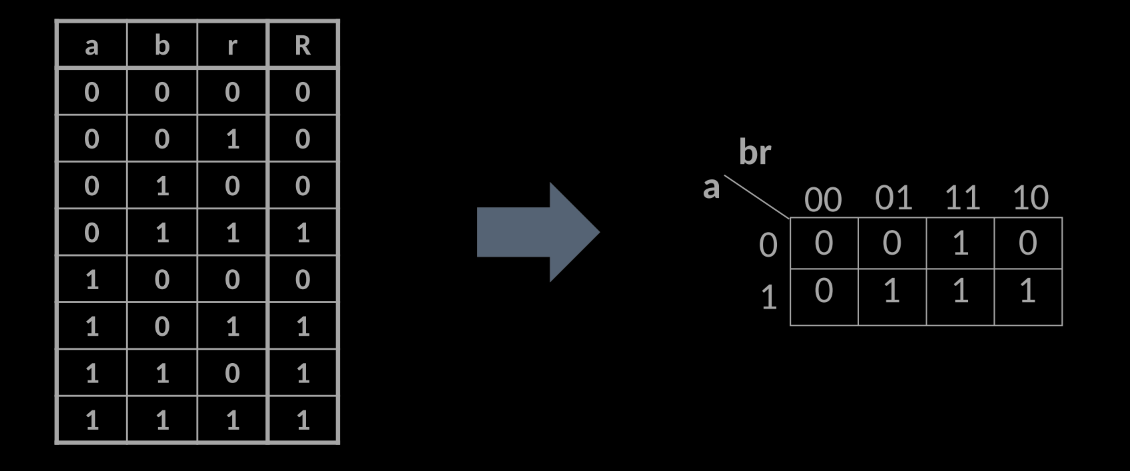
\includegraphics[scale=0.53]{karnfulladd.png}
\end{center}
\subsubsection{Celle adiacenti}
Due celle in una mappa di Karnaugh si dicono adiacenti se le loro coordinate differiscono di un solo bit. In una mappa che descrive una funzione di $n$ variabili ogni cella ha $n$ celle adiacenti.
\vspace{0.2cm}\\
Regola grafica per l'adiacenza: sono adiacenti celle aventi un lato in comune o poste all'estremità di una stessa riga o colonna.
\begin{center}
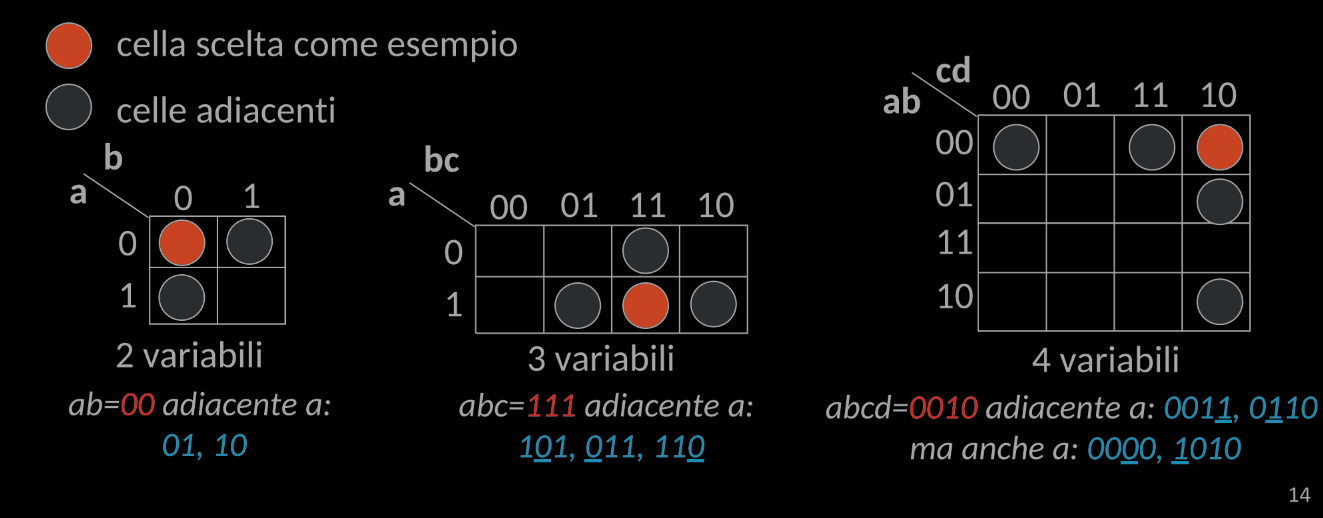
\includegraphics[scale=0.53]{cellead.png}
\end{center}
\subsubsection*{Estensione delle mappe a 5 e a 6 variabili}
\begin{center}
    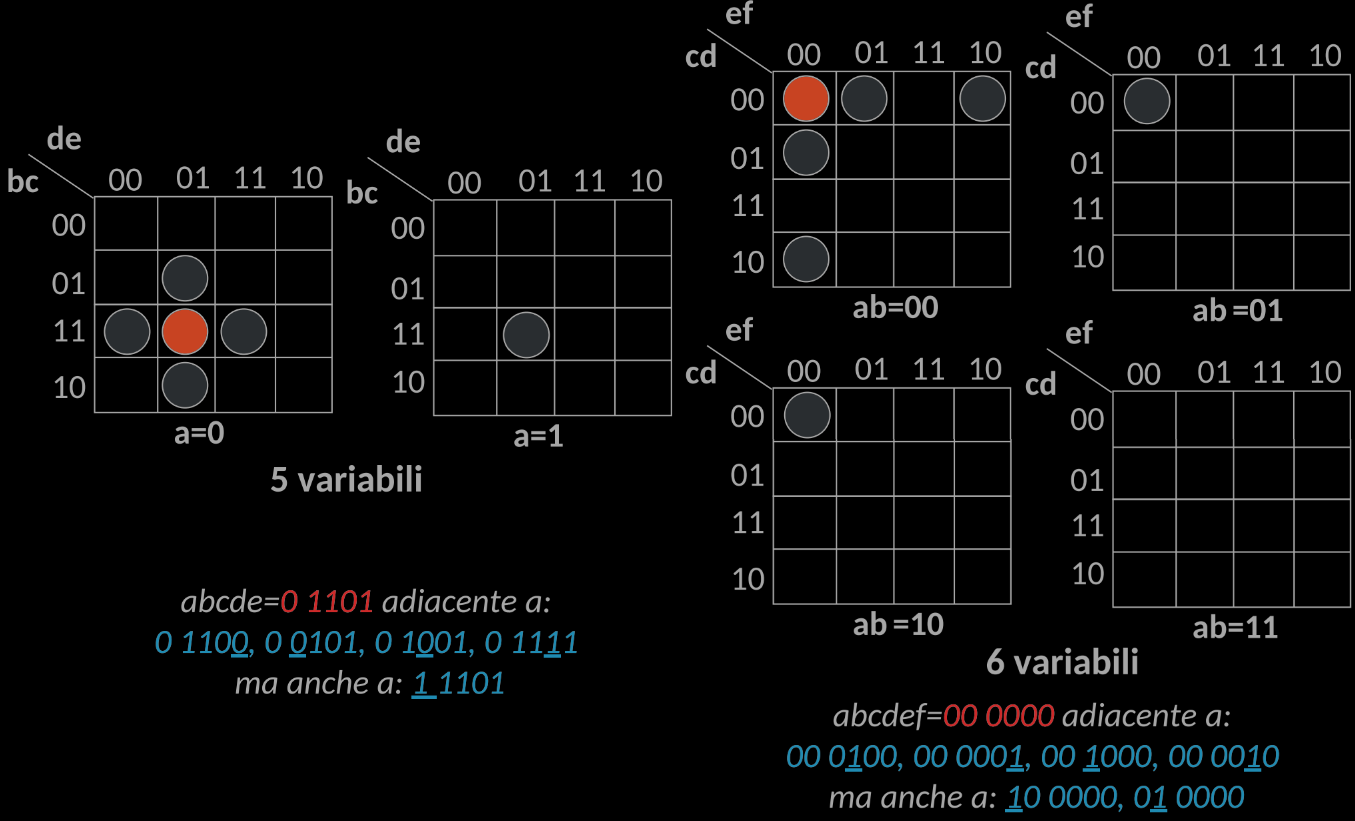
\includegraphics[scale=0.53]{celle5-6.png}
\end{center}
Ulteriore regola di adiacenza: sono adiacenti celle che occupano la stessa posizione in sotto-mappe adiacenti.
\subsubsection{Manipolazione algebrica per via grafica}
Ma perché è importante individuare celle adiacenti?
\begin{center}
    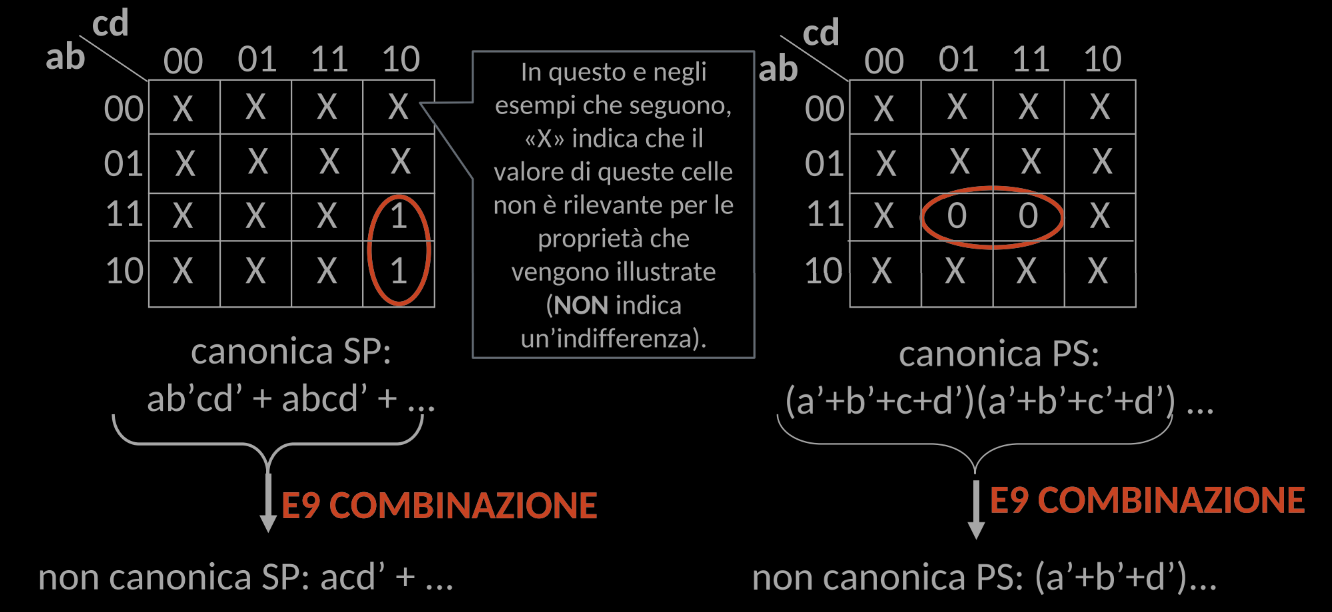
\includegraphics[scale=0.48]{cellad2.png}
\end{center}
Due termini di una espressione canonica (SP o PS) corrispondenti a configurazioni che individuano celle adiacenti sono equivalenti ad un unico termine con un letterale in meno (quello che cambia valore).
\subsection{Raggruppamenti rettangolari (RR)}
Un raggruppamento rettangolare di ordine $p$ è un insieme di $2^p$ celle di una mappa all'interno del quale ogni cella ha esattamente $p$ celle adiacenti.\\
\textbf{N.B.} il numero di celle deve essere per forza una potenza di 2.
\vspace{0.3cm}\\
Un RR di ordine $p$ costituito da celle contenenti valore 1, ed eventualmente condizioni di indifferenza, individua un \textbf{implicante} della funzione. Nel prodotto compaiono le sole $(n-p)$ variabili che rimangono \textbf{costanti} nelle coordinate del RR, in forma vera se valgono 1, in forma complementata se valgono 0.
\vspace{0.2cm}\\
Un RR di ordine $p$ costituito da celle contenenti valore 0, ed eventualmente condizioni di indifferenza, individua un \textbf{implicato} della funzione. Nella somma compaiono le sole $(n-p)$ variabili che rimangono costanti nelle coordinate del RR, in forma vera se valgono 0, in forma complementata se valgono 1.
\vspace{0.2cm}\\
Un RR formato da celle contenenti valore 1 o indifferenza e non interamente incluso in un RR di ordine superiore individua un implicante primo.
\vspace{0.2cm}\\
Un RR formato da celle contenenti valore 0 o indifferenza e non interamente incluso in un RR di ordine superiore individua un implicato primo.
\begin{center}
    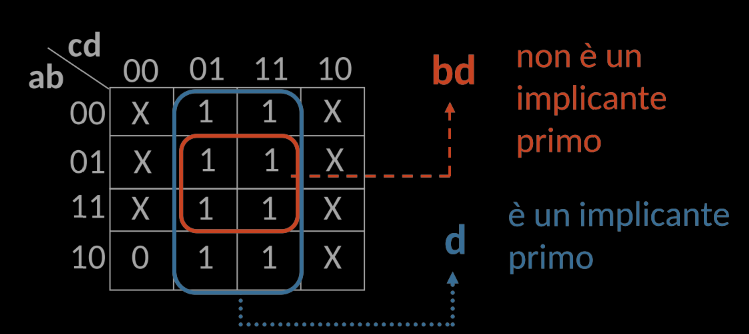
\includegraphics[scale=0.55]{raggimpl.png}
\end{center}
\begin{center}
    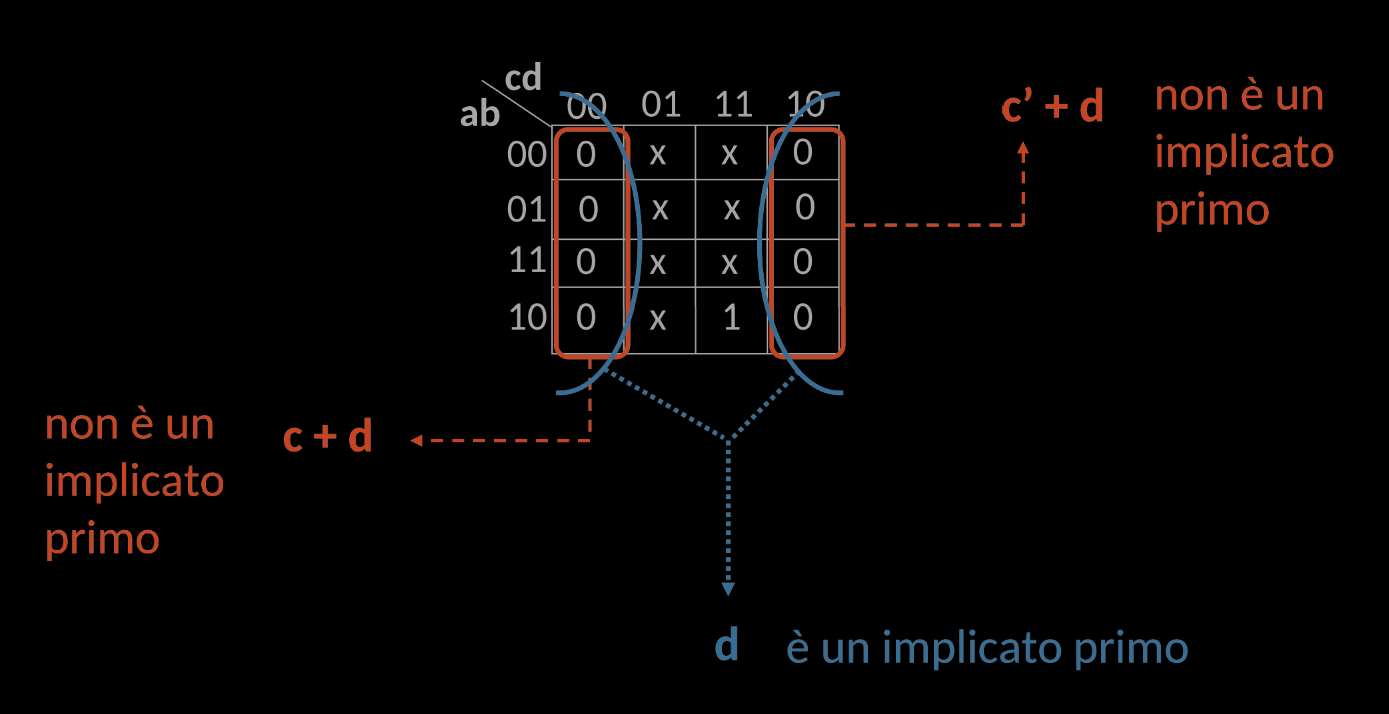
\includegraphics[scale=0.45]{spRR}
\end{center}
\subsubsection{Individuazione grafica dei termini ridondanti}
Un RR le cui celle sono tutte incluse in altri RR
non deve essere usato nell'espressione minima, per la proprietà del \textit{consenso}. Corrispondono a implicanti (implicati) primi, ma non essenziali.
\begin{center}
    \includegraphics[scale=0.55]{ridond.png}
\end{center}
\subsection{Copertura minima}
La \textit{copertura} di una funzione su una mappa è un insieme di RR la cui unione racchiude tutte le celle contenenti o valore 1 (copertura degli uni) o valore 0 (copertura degli zeri), ed eventualmente celle con valore indifferente.
\vspace{0.2cm}\\
Una copertura degli uni (zeri) individua una espressione SP (PS) che fornisce una possibile struttura per realizzare la funzione assegnata tramite la mappa. Gli implicanti (o implicati) che appaiono nell'espressione sono individuati dai raggruppamenti componenti la copertura.
\vspace{0.2cm}\\
La \textit{copertura minima} è una copertura costituita dal minimo numero possibile di RR di dimensione massima e corrispondente all'espressione minima.
\vspace{0.2cm}\\
Quando una o più celle possono essere coperte con più RR della stessa dimensione (come le celle abcd=0101 e 0111 nell'esempio successivo), devo considerarli tutti e scegliere quelli essenziali ($a'bd$ in questo esempio)
\begin{center}
    \includegraphics[scale=0.55]{copertura.png}
\end{center}
Altri esempi:
\begin{center}
    \includegraphics[scale=0.55]{escoper.png}
\end{center}
\begin{center}
    \includegraphics[scale=0.55]{escoper2.png}
\end{center}
\subsection{Individuazione grafica dell'espressione minima}
A partire dalla mappa che descrive la funzione occorre determinare la copertura minima e da questa la corrispondente espressione minima. Il procedimento è per suo natura non sistematico e richiede l'abilità di chi lo esegue.\\
È tuttavia possibile delineare una sequenza di passi che consentono di individuare la copertura minima:
\begin{enumerate}
    \item Si decide se cercare l'espressione di tipo SP o PS e ci si predispone di conseguenza a coprire gli uni o gli zeri.
    \begin{center}
        \includegraphics[scale=0.55]{ind1}
    \end{center}
    \item Si cerca di individuare tra le celle da coprire una cella che possa essere racchiusa in un solo RR e lo si traccia di dimensione massima, annotando il termine corrispondente. Se la funzione è incompleta il RR può contenere anche condizioni di indifferenza.
    \begin{center}
    \includegraphics[scale=0.55]{ind2}
    \end{center}
    Si ripete fino a quando è possibile il passo 2, tenendo conto della possibilità di coprire anche celle incluse in RR già tracciati.
    \begin{center}
    \includegraphics[scale=0.55]{ind2.1.png}
    \end{center}
    \item Si prendono in considerazione le celle ancora da coprire e se ne sceglie la copertura migliore, tenendo conto come al solito della possibilità di coprire celle già coperte e condizioni di indifferenza.
    \begin{center}
        \includegraphics[scale=0.55]{indes3}
    \end{center}
    \item si ripete il passo 3 fino a soddisfare la condizione di copertura.
    \begin{center}
    \includegraphics[scale=0.55]{ind4}
    \end{center}
\end{enumerate}
\subsubsection{Sintesi minima di un encoder}
L'\textit{encoder} converte codice "1 su N" in codice binario; per esempio un encoder di codice "1 su 3" a numero binario è fatto così:
\begin{center}
    \includegraphics[scale=0.52]{encoder3.png}
\end{center}
Mappa di Karnaugh e espressione minima di $z_1$:
\begin{center}
    \includegraphics[scale=0.55]{Z1.png}
\end{center}
Mappa di Karnaugh e espressione minima di $z_0$:
\begin{center}
    \includegraphics[scale=0.55]{Z2.png}
\end{center}
\subsection{Analisi con mappe}
\subsubsection{Uso delle mappe in fase di analisi}
\begin{enumerate}
    \item Si scrive l'espressione associata allo schema e, se necessario, la si manipola fino ad ottenere una espressione SP o PS:
    \begin{center}
        \includegraphics[scale=0.45]{mappeanalisi1.png}
    \end{center}
    \item Si predispone una mappa di dimensioni adeguate e si tracciano sulla mappa i RR che corrispondono ai termini dell'espressione
    \begin{center}
        \includegraphics[scale=0.45]{mappeanalisi2.png}
    \end{center}
    \item Nelle celle coperte da un RR si indica il valore 1 se l'espressione è SP, 0 se è PS; nelle celle non coperte da RR si inserisce 0 nel caso SP, 1 nel caso PS:
\end{enumerate}
\subsection{Sintesi a NAND}
\subsubsection{Scrivere NOT AND e OR da NAND}
Ricordiamo la tabella della verità del NAND:
\begin{center}
    \includegraphics[scale=0.5]{tdvnand.png}
\end{center}
\begin{itemize}
    \item NOT: $$x \uparrow x = x'$$
    \item AND: $$ (x \uparrow y)' = xy $$
    \item OR: $$ x+y=(x'y')' = x' \uparrow y' $$
\end{itemize}
\subsubsection{Sintesi con NAND}
La sintesi a NAND può essere effettuata trasformando un'espressione SP(o SPS, SPSP,...) che descrive la funzione assegnata in una nuova espressione contenete esclusivamente operatori NAND.
\vspace{0.2cm}\\
Prendiamo una funzione d'esempio:
$$ F = a \cdot b + \overline{c} \cdot d + e \cdot \overline{f} +g $$
definizione dell'operatore NAND: $ \overline{a \uparrow b }= ab$
$$ F = (\overline{a \uparrow b }) + \overline{(\overline{c} \uparrow d)} + \overline{(e \uparrow \overline{f})} + g $$
 seconda legge di De Morgan: $\overline{a} + \overline{b} = \overline{ab}$
$$ F = \overline{\Big( (a \uparrow b) \cdot (\overline{c} \uparrow d) \cdot (e \uparrow \overline{f}) \cdot \overline{g} \Big)} $$
definizione di NAND
$$ F = (a \uparrow b) \uparrow (\overline{c} \uparrow d) \uparrow (e \uparrow \overline{f}) \uparrow \overline{g} $$
\subsubsection{Algoritmo per la sintesi a NAND}
\begin{enumerate}
    \item Si parte da un'espressione e s introducono gli operatori $"\cdot"$ e le parentesi non indicati esplicitamente.
    \item Si sostituisce il simbolo $"\uparrow"$ ad ogni simbolo $"\cdot"$
    \item Si sostituisce il simbolo $"\uparrow"$ ad ogni simbolo $"+"$ e si complementano le variabili \textbf{\underline{singole}} (non i prodotti) affiancate a tale simbolo senza aggiungere o togliere parentesi.
    \item (Opzionale) Se compaiono segnali di ingresso in forma negata e non sono disponibili, si sostituiscono con il NAND del segnale in forma vera.
\end{enumerate}
\subsubsection*{Esempio di una sintesi a NAND di un EX-OR}
$$ U = a b' + a'b $$
$$ U = (a \cdot b') + (a' \cdot b) $$
$$ U = (a \uparrow b') \uparrow(a' \uparrow b) $$
$$ U = \big( a \uparrow (b \uparrow b) \big) \uparrow \big( (a \uparrow a) \uparrow b \big) $$
\subsubsection*{Sintesi a NAND di un Selettore a 2 vie}
$$ U = A'I_0 + A I_1 $$
$$ (A' \cdot I_0) + (A \cdot I_1) $$
$$ U = (A' \uparrow I_0) \uparrow (A \uparrow I_1) $$
$$ U = \big( (A \uparrow A) \uparrow I_0 ) \big) \uparrow (A \uparrow I_1) $$
Reti a NAND o NOR, utilizzando un unico tipo di gate, riducono spesso il numero di circuiti SSI necessari. \\
N.B. SSI sta per Small Scale Integration.
\subsection{Sintesi con NOR}
La sintesi "a NOR" può essere effettuata trasformando un' espressione PS (PSP, PSPS,...) che descrive la funzione assegnata in una nuova espressione contente esclusivamente operatori $\downarrow$.
\vspace{0.1cm}\\
Vediamo un esempio:
$$ F = (\overline{a} + \overline{b}+c) \cdot (\overline{d} +e) \cdot \overline{f} \cdot g $$
Definizione dell'operatore NOR: $\overline{a \downarrow b} = a +b $
$$ F = \overline{(\overline{a }\downarrow \overline{b} \downarrow c) }\cdot \overline{(\overline{d} \downarrow e) }\cdot \overline{f} \cdot g$$
I legge di De Morgan: $\overline{a} \cdot \overline{b} = \overline{a+b} $
$$ F = \overline{(\overline{a }\downarrow \overline{b} \downarrow c) + (\overline{d} \downarrow e) + f + \overline{g}} $$
Definizione operatore NOR
$$ F = (\overline{a }\downarrow \overline{b} \downarrow c) \downarrow (\overline{d} \downarrow e) \downarrow f \downarrow \overline{g} $$
N.B. Il NOR non è associativo, le parentesi sono fondamentali.
\subsubsection{Algoritmo per la sintesi a NOR}
\begin{enumerate}
    \item Si parte da un'espressione PS, PSP, PSPS,... e si introducono gli operatori $"\cdot"$ e le parentesi non indicati esplicitamente.
    \item Si sostituisce il simbolo $\downarrow $ a ogni simbolo $"+"$
    \item Si sostituisce il simbolo $"\downarrow"$ ad ogni simbolo $"\cdot"$ e si complementano le variabili singole (non le somme) affiancate a tale simbolo senza aggiungere o togliere parentesi.
    \item (Opzionale) Se compaiono segnali di ingresso in forma negata e non sono disponibili, li sostituisco con il NOR del segnale in forma vera.
\end{enumerate}
\subsubsection*{Esempio: sintesi a NOR di un "equivalence"}
\begin{center}
    \includegraphics[scale=0.55]{equivalence.png}
\end{center}
\section{Sintesi tramite decoder, Multiplexer e ROM}
\subsection{Introduzione}
Sono disponibili nella forma di componenti elementari anche reti più complesse delle semplici "famiglie di gate" viste in precedenza. Tali reti risultano particolarmente utili per il progettista logico, in quanto rappresentano i blocchi base per risolvere problemi più complessi. Vedremo ora l’utilizzo di alcune di tali reti al fine della sintesi combinatoria.
\subsection{Decoder e sintesi con decoder e OR}
\subsubsection{Esempio Deocder 3:8}
Un decoder 3:8 è una rete combinatoria che converte da numero binario a 3 bit e codice "1 su 8"($2^3$). ha quindi 3 ingressi e 8 uscite. Per convenzione si usano le prime 3 lettere dell'alfabeto per indicate gli ingressi, con la A usata per la cifra meno significativa. Ogni uscita ha solo una configurazione degli ingressi per cui vale 1, quella che codifica il numero dell’uscita stessa. Quindi la sintesi canonica (e anche minima) prevede quell'unico mintermine nell'espressione.
\begin{center}
    \includegraphics[scale=0.7]{decoder3:8.png}
\end{center}
\subsubsection{Il decoder generico DEC}
Il DEC è una rete di trascodifica da codice binario a $n$ bit a codice 1 su $2^n$. Gli $n$ ingressi vengono anche indicati come indirizzi (A, address), con $A_0$ indirizzo di minor peso.
L’indice $i$ dell’uscita $U_i$ attivata è pari al numero rappresentato dalla configurazione binaria degli ingressi: $ i = A_{n-1} \cdot 2^{n-1} + ... + A_1 \cdot2^1 + A_0 \cdot 2^0 $.
\begin{center}
    \includegraphics[scale=0.7]{tabDec.png}
\end{center}



\subsubsection{Decoder 2:4 e 3:8}
\begin{center}
    \includegraphics[scale=0.35]{decoder 2:4 e 3:8.png}
\end{center}



\subsubsection{Effetto di carico: Fan-out}
L'uscita di un gate è caratterizzata da un fan-out, ovvero un numero massimo di gate a cui può essere collegata. Il fan-out di un gate dipende dalla tecnologia con cui è realizzato ed è generalmente alto ($>10$), ma è comunque limitato. 
\vspace{0.3cm}\\
Possono sorgere problemi quando quando si connette un'uscita di un gate con un componente più complesso, come ad esempio un DEC 3:8; in un caso del genere non è chiaro, senza conoscere la struttura interna del componente, quanto fan-out consuma quel circuito e quanto ne rimane.
\begin{center}
    \includegraphics[scale=0.55]{es3:8.png}
\end{center}
C'è però una soluzione: si possono usare due NOT in cascata per avere il segnale in forma vera e negata senza far consumare più carico all'ingresso.
\subsubsection{Fan-in}
I gate disponibili hanno un numero di ingressi limitato (spesso 2, tipicamente non più di 8) detto fan-in. Per eseguire operazioni di somma e prodotto logico con un più elevato numero di ingressi si può sfruttare la proprietà associativa di AND, OR e EX-OR:
\begin{center}
    \includegraphics[scale=0.5]{fan-in1.png}
\end{center}
Nel caso di gate NAND e NOR (per i quali non vale la proprietà associativa) si deve invece applicare un NOT a valle di un AND/OR con il fan-in desiderato:
\begin{center}
    \includegraphics[scale=0.5]{fan-in2.png}
\end{center}
\subsubsection{Sintesi del Full Adder con Decoder e Or}
Utilizzando opportunamente Decoder e gate OR si può sintetizzare qualsiasi espressione in forma canonica SP. Questa non è una sintesi di costo minimo, non servono mappe e ha un tempo di progettazione quasi nullo. Da ricordare che bisogna collegare gli ingressi ai bit di indirizzo nell’ordine usato per definire i mintermini.
\begin{center}
    \includegraphics[scale=0.55]{sintesiFullAdder.png}
\end{center}
Codesto è un circuito a due livelli, quindi ha la stessa velocità di elaborazione delle reti minime SP/PS.
\subsection{Il circuito integrato DECODER}
\subsubsection{Realizzazione modulare di un Decoder 4:16}
Non è possibile realizzare decoder $n>5$ perché il numero di componenti e di uscite cresce esponenzialmente con $n$.\\
Però si può utilizzare la composizione modulare, dato che il prodotto logico gode della proprietà associativa.
\vspace{0.2cm}\\
Esempio:
$$ U_9 = EN_2 \overline{B} A = (D \overline{C}) \overline{B} A = D \overline{C} \overline{B} A $$
\begin{center}
    \includegraphics[scale=0.7]{Dec4:16.png}
\end{center}
\subsection{Multiplexer}
\subsubsection{Selettore a 2 vie}
Un selettore è l'equivalente Hardware di un {\fontfamily{lmtt}\selectfont if}: permette di decidere, tramite un segnale A, quale tra le due vie d'ingresso $I_0 I_1$ sarà replicata dall'uscita. Per convenzione, per rappresentare un multiplexer si usa un trapezio invece del solito rettangolo.\\
La tabella della verità (in forma di mappa di Karnaugh) e l’equazione SP risultante sono le seguenti:
\begin{center}
    \includegraphics[scale=0.6]{TDVMulti.png}
\end{center}
\subsubsection{Multiplexer (MUX) generico}
Il concetto di selettore può essere generalizzato a $n$ bit di indirizzo
Gli $n$ bit di indirizzo selezionano uno tra i $2^n$ ingressi detti "vie" o anche "bit di programmazione" a seconda dell’uso che si fa del MUX (come selettore o generatore di funzioni). Ovviamente al crescere di $n$ cresce esponenzialmente il numero delle vie.\\
L’ingresso replicato sull’uscita si determina dai bit di indirizzo secondo la stessa relazione vista per il DEC.
\subsubsection{Multiplexer a $2^n$ vie}
La sua struttura può essere dedotta generalizzando quella di un MUX a 2 vie: se il MUX a 2 vie ha 2 AND a 2 ingressi (uno per la via e 1 per l’indirizzo) e un OR a 2 ingressi, il MUX a $2^n$ vie ha $2^n$ AND a $n+1$ ingressi ($n$ bit di indirizzo più 1 via di ingresso) e 1 OR a $2^n$ ingressi.
\begin{center}
    \includegraphics[scale=0.9]{MUX2n.png}
\end{center}
\subsubsection{Teorema di espansione di Shannon}
Data una funzione $F$ di $n$ variabili binarie, vale la relazione (in forma SP)
$$ F(x_1,...,x_i,...,x_n) = x_i F(x_1,...,1,...,x_n) + \overline{x_i} F(x_1,...,0,...,x_n)  $$
che può essere scritta anche in forma PS in questo modo
$$ F(x_1,...,x_i,...,x_n) = 
\Big(x_i + F(x_1,...,0,...,x_n) \Big) \cdot \Big( \overline{x_i} + F(x_1,...,1,...,x_n) \Big) $$
\subsubsection{Espressioni generali}
Applicando ripetutamente il teorema di espansione di Shannon è possibile dedurre le seguenti espressioni generali:
\begin{itemize}
    \item Caso SP: ogni funzione di $n$ variabili è descritta da una espressione in cui compaiono, in somma logica, tutti i mintermini di $n$ variabili ciascuno in prodotto logico con il valore della funzione quando in ingresso compare la configurazione del mintermine
    $$ F(x_1,x_2,...,x_n) = \sum^{2^n -1}_{i=0} m(i) \cdot F(i) $$
    dove $m(i)$ è il mintermine di $n$ bit e $F(i)$ è il valore della funzione relativo alla configurazione per cui $m(i) = 1$
    \item Caso PS: ogni funzione di $n$ variabili è descritta da una espressione in cui compaiono, in prodotto logico, tutti i maxtermini di $n$ variabili ciascuno in somma logica con il valore della funzione quando in ingresso compare la configurazione del maxtemine
    $$ F(x_1,x_2,...,x_n) = \prod_{i=0}^{2^n -1} \big( M(i) + F(i) \big)$$
    dove $M(i)$ è il maxtermine di $n$ bit e $F(i)$ è il valore della funzione relativo alla configurazione per cui $M(i)=0$.
\end{itemize}
\subsubsection{Il MUX come rete programmabile}
Il MUX si adatta bene a realizzare l’espressione precedente nel caso SP. Siccome abbiamo $n$ variabili occorre un MUX con $n$ bit di ingresso. Il MUX viene qui utilizzato come generatore di funzioni (componente programmabile a seconda della funzione che si vuole realizzare).
\vspace{0.2cm}\\
Di seguito uno schema su come realizzare un MUX di questo tipo.
\begin{center}
    \includegraphics[scale=0.35]{ProgMUX.png}
\end{center}
\subsubsection*{Sintesi di un Full Adder con MUX}
Riporto la tabella della verità di un Full Adder:
\begin{center}
    \includegraphics[scale=0.27]{fulladderTdv.png}
\end{center}
Riproduco in ingresso al MUX i contenuti della tabella della verità.\\
ATTENZIONE: collegare gli ingressi al bit di indirizzo giusto\\
In questo modo massimizzo ancora il criterio della rapidità di progetto. La velocità di elaborazione rimane invece quella delle reti minime (come si vede dalla realizzazione del MUX).
\begin{center}
    \includegraphics[scale=0.37]{MUXfa.png}
\end{center}
N.B. Dato che il numero di vie cresce esponenzialmente con il numero di bit di indirizzo i MUX sotto forma di circuito integrato hanno al più 16 bit di programmazione (il numero di pin di un circuito integrato è limitato).
\subsubsection{Sintesi a MUX di funzioni di 4 variabili}
La composizione è possibile anche con MUX, usando il teorema di espansione. Per rendere coerenti i bit di programmazione con la tabella della verità, è consigliabile far corrispondere gli indirizzi dei dispositivi a valle ai bit di maggior peso (es. Q3).
\begin{center}
    \includegraphics[scale=0.37]{MUX4var.png}
\end{center}
\subsection{Reti Programmabili}
\subsubsection{VLSI}
Le reti in Large Scale Integration e Very Large Scale Integration sono costituite da milioni di gate integrati (tutti in un unico chip). Ciò comporta costi molti onerosi in tutte le sue fasi di realizzazione; per ammortizzarli ne occorre un vasto impiego.
\vspace{0.2cm}\\
La realizzazione di una rete VLSI ad hoc per uno specifico problema è quindi impossibile (richiederebbe dei costi enormi), perciò si rende necessaria la possibilità di programmazione. Questo permette di ammortizzare i costi elevati attraverso grandi volumi di vendita dello stesso prodotto.
\subsubsection{Reti combinatorie programmabili}
Le reti combinatorie programmabili hanno la caratteristica di presentare diverse relazioni ingresso/uscita selezionabili mediante l’attribuzione di una determinata configurazione di valori ad un gruppo di segnali interni detti bit di programmazione.
\begin{center}
    \includegraphics[scale=0.5]{retiProg1.png}
\end{center}


\subsection{Memorie a sola lettura (ROM)}
Una \textbf{\color{cyan} Read Only Memory} è proprio un circuito che realizza una memoria a sola lettura, ovvero che contiene ad ogni indirizzo un dato fissato.
\\
In una ROM possiamo interpretare i bit di ingresso come bit di indirizzo: $A_0,...,A_{n-1}$ e bit di uscita come bit di dato: $D_0,...,D_{k-1}$. Una ROM è quindi una \textbf{memoria} in grado di memorizzare $2^n$ dati, ciascuno di $k$ bit.\\
Una ROM in grado di memorizzare $N$ dati (formati da $k$ bit) sarà dunque indirizzabile mediante $n = log_2 N$ bit di indirizzo.




\section{Aritmetica binaria}


\subsection{Aritmetica binaria senza segno}
Somme e sottrazioni tra numeri binari si eseguono su carta esattamente come abbiamo imparato a fare con i numeri decimali alla scuola elementare. L'unica differenza è che con carta e penna posso sempre aggiungere cifre, nei sistemi digitali ho un numero fisso e finito di cifre disponibili. Infatti la somma di due numeri a $n$ bit può non essere rappresentabile con il numero di bit disponibile (\textbf{\color{cyan} overflow}).
\vspace{0.1cm}\\
Per esempio con cifre binarie posso rappresentare numeri senza segno compresi tra 0 e 63($2^6-1$). Se la somma è minore di 63 il risultato è valido, altrimenti ho overflow è il risultato non è valido.\\
La condizione di overflow è segnalata dall’ultimo riporto (\textbf{\color{cyan} carry out}).
\begin{center}
    \includegraphics[scale=0.35]{aritmetica 1.png}
\end{center}



\subsection{Full Adder e Half Adder}
La rete che realizza la somma di due bit nel caso generale con riporto viene detta {\color{cyan}Full Adder}. Quando ho solo due bit in input invece si parla di {\color{cyan}Half Adder}.
\vspace{0.1cm}\\
L’Half Adder è realizzabile con un EX-OR per la somma e un AND per il riporto, come si vede dalla parte in grigio della tabella della verità di un full adder.
\vspace{0.1cm}\\
Il full adder è realizzabile a partire da due half adder e un OR: la somma di 3 bit è la somma dei primi due (EX-OR) che viene poi sommata al terzo (altro EXOR); il riporto complessivo vale 1 se ho riporto nella prima somma OR nella seconda.
\begin{center}
    \includegraphics[scale=0.35]{TDV Full Adder.png}
    \includegraphics[scale=0.35]{Full Adder.png}
\end{center}


\subsubsection{Adder a $n$ bit}
Per realizzare un sommatore a $n$ bit, è sufficiente disporre in serie un Half Adder e $n-1$ Full Adder. Ogni Half o Full Adder realizza una della colonne della somma in colonna. Il riporto dell’ultimo full adder rappresenta il bit di {\color{cyan}carry out} $c_{out}$ che indica la validità o meno del risultato.
\begin{center}
    \includegraphics[scale=0.35]{adder n bit.png}
\end{center}
\vspace{0.3cm}
Se si sostituisce l’unico Half Adder con un Full Adder si ottiene un sommatore con un ingresso aggiuntivo di carry in $c_{in}$, che può essere usato per disporre Adder a $n$ bit in serie e realizzare sommatori con un numero di ingressi maggiore di $2n$, ovvero per sommare numeri con un numero di bit maggiori di $n$.



\subsection{Complemento a 1 e complemento a 2}
Definizione di {\color{cyan} complemento a $\beta -1$} di un numero in base $\beta$: dato un numero A rappresentato a $n$ cifre il complemento a $\beta -1$ di tale numero è $(\beta ^n  -1) - A $
Nel caso del sistema binario, il complemento a 1 equivale all’operatore NOT applicato ad ogni cifra.
\vspace{0.1cm}\\
Definizione di {\color{cyan}complemento a $\beta$} di un numero in base $\beta$: dato un numero A rappresentato da $n$ cifre il complemento a $\beta$ di tale numero è $\beta ^n -A$.
\vspace{0.1cm}\\
\textbf{Esempi:}
\begin{itemize}
    \item il complemento a 9 (10 - 1) di $(001234)_{10}$ è 
    $$ (10^6-1)-001234 = 999999-001234=998765 $$
    \item il complemento a 1(2-1) di $(001110)_2$ è
    $$ (2^6-1)-001110 = 111111 - 001110 = 110001 $$
\end{itemize}

Possiamo calcolare il complemento a $\beta$ sommando 1 al complemento a $\beta - 1$, infatti nel caso binario si ottiene la regola secondo cui il {\color{cyan}complemento a 2} si un numero A è dato da $NOT(A)+1$.
\vspace{0.1cm}\\
\textbf{Esempi:}
\begin{itemize}
    \item il complemento a 2 di $(001110)_2$ è 
    $$ 2^6-001110 = 1000000 - 001110= 110010 $$
    o anche
    $$ NOT (001110) + 1 = 110001 + 1 = 11001 $$
\end{itemize}
Un modo equivalente di calcolarlo è quello di lasciare invariato il numero fino al primo 1 partendo da destra incluso, e complementare tutte le altre cifre.\\
\textbf{N.B.} Se calcolo il complemento a 2 di un complemento a 2 ottengo il numero di partenza.
\vspace{0.3cm}\\
A cosa serve la rappresentazione in complemento a 2?
\begin{enumerate}
    \item \textbf{\color{cyan} A implementare la sottrazione come somma}, quindi ad usare lo stesso semplice ed efficiente circuito che abbiamo già sintetizzato per eseguire somme e sottrazioni
    \item \textbf{\color{cyan} A rappresentare i numeri con segno quando sono negativi} in maniera tale che le operazioni su di essi possano essere eseguite in modo efficiente
\end{enumerate}



\subsubsection{Sottrazione tra numeri senza segno}
Dati due numeri binari senza segno a $n$ bit A e B con $A>B$, si può calcolare $A-B$ sommando A al complemento a 2 di B e ignorando il carry out uguale a 1. Infatti, il complemento a 2 di B è $2^n-B$, quindi il risultato della somma è $(A-B)+2^n$.\\
Poiché il complemento a 2 si ottiene come $NOT(B) + 1$, è sufficiente negare B in ingresso all’adder a $n$ bit e settare $c_{in}=1$.
\begin{center}
    \includegraphics[scale=0.38]{sottrazione.png}
\end{center}
Se $A - B < 0$, il risultato non è rappresentabile come numero senza segno perché il risultato della somma è $<2^n$ e il carry out risulta 0.


\subsection{Adder e Subtracter}
Realizziamo un circuito comandato da un bit di input $S/D'$ che: quando $S=1$ presenta sulle $n$ uscite $U[n-1. . 0] $ la somma dei due numeri in input $A[n-1. . 0]$ e  $B[n-1. . 0]$ a $n$ bit; quando $S = 0 $ riporta la sottrazione $A-b$; in entrambi i casi asserisce il bit di uscita $CF$ (carry flag) se si è verificato overflow nello svolgimento dell’operazione.\\
\textbf{N.B.} Le uscite che indicano il verificarsi di condizioni particolari nel risultato prendono il nome di flag.
\vspace{0.1cm}\\
Questa è la logica dietro il nostro circuito:
\begin{center}
    \includegraphics[scale=0.35]{adder-sub.png}
\end{center}
Quindi la sua realizzazione sarà:
\begin{center}
    \includegraphics[scale=0.35]{adder-sub2.png}
\end{center}



\subsection{Numeri con segno}
Nelle reti logiche per i numeri con segno viene utilizzata la rappresentazione con \textbf{\color{cyan} complemento a 2}.\\
I numeri rappresentabili attraverso il complemento a 2 appartengono all'intervallo asimmetrico
$$ - 2^{n-1} \leq A \leq 2^{n-1}-1 $$
Viene usata proprio questa rappresentazione perché operazioni elementari tra numeri rappresentati in complemento a 2 danno come risultato ancora numeri in complemento a 2, cosa non vera per la rappresentazione in segno e valore assoluto.
\subsubsection*{Estensione di un numero in complemento a 2}
Per estendere il numero di bit di un numero rappresentato in complemento a 2, si deve replicare il bit più significativo. Per esempio, per passare da 5 a 7 bit:
$$ (11100)_2 = -4 \rightarrow (\underline{111}1100)_2 = -64 + 32 + 16 + 8 + 4= -16 + 8 + 4 = (-4)_{10} $$
$$ (01100)_2 = 8 + 4 = 12 10 \rightarrow (\underline{00}01100)_2 = 8 + 4 = (12)_{10} $$



\subsubsection{Aritmetica binaria con segno}
Anche per i numeri con segno la somma di due numeri a $n$ bit può non essere rappresentabile con il numero di bit disponibile (\textbf{\color{cyan}overflow}).\\
Per i numeri con segno la situazione di overflow è individuabile controllando se gli operandi hanno segno concorde e diverso da quello del risultato (ovvero, per esempio, sommo due numeri positivi e ottengo un numero negativo). Ciò equivale a verificare se
$$ a_{n-1} = b_{n-1}\text{ AND } b_{n-1} \neq s_{n-1} $$
\begin{center}
    \includegraphics[scale=0.35]{aritmetica con segno.png}
\end{center}



\subsubsection{Adder modificato per sottrazione di numeri con segno}
Per gestire numeri con segno, quindi, aggiungiamo un segnale di uscita di overflow all’adder a $n$ bit che avevamo definito.
\begin{center}
    \includegraphics[scale=0.35]{n bit adder modificato.png}
\end{center}




Infine, come per i numeri senza segno, per sottrarre due numeri con segno, è sufficiente eseguire il complemento a due del sottraendo e sommarli. Infatti, eseguendo il complemento a 2 si cambia segno al numero e quindi la somma esegue la sottrazione voluta.\\
Per ottenere un generico circuito che esegue somme e sottrazioni tra numeri con e senza segno, quindi, è possibile usare quello visto in precedenza. La condizione di overflow sarà segnalata dall’uscita CF (carry flag) o da OF (overflow flag) a seconda che sia stata eseguita un’operazione tra numeri con segno o senza.
\begin{center}
    \includegraphics[scale=0.35]{n bit adder complemento.png}
\end{center}





\subsection{Arithmetic Logic Unit (ALU)}
La codifica dei numeri con e senza segno e i circuiti che abbiamo visto sono la base per costruire le cosiddette \textbf{\color{cyan} Arithmetic Logic Unit (ALU)}.\\
Le ALU sono macchine combinatorie in grado di eseguire operazioni aritmetiche (somma, sottrazione, complemento a 2, scorrimento a destra o sinistra, …) e logiche (bit per bit AND, OR, XOR, …) sui due operandi in base al codice operativo (op-code) in ingresso. Oltre a fornire il risultato dell’operazione, indicano anche attraverso una serie di flag il verificarsi di particolari condizioni nel risultato stesso.\\
Le ALU sono il motore di un microprocessore e le CPU moderne hanno anche più di una ALU per core.
\begin{center}
    \includegraphics[scale=0.35]{alu.png}
\end{center}
Il circuito di una ALU che può eseguire operazioni logiche o aritmetiche ($M=1$ per operazioni aritmetiche, $M=0$ per operazioni logiche) è il seguente:
\begin{center}
    \includegraphics[scale=0.35]{alu circuito.png}
\end{center}



\subsection{Adder e Carry Lookahead}
Il limite principale dell’adder realizzato come disposizione in serie di Full Adder è la lentezza, dovuta alla catena dei riporti. Questa realizzazione viene anche detta \textbf{\color{cyan} ripple-carry adder}.\\
Ogni FA infatti impiega $2 \tau _p$ per portare a regime il riporto in uscita da quando è a regime il riporto in ingresso. Se eseguo operazioni tra dati a 64 bit, nel caso peggiore ho quindi il risultato aggiornato dopo 128 $\tau _p$.
\vspace{0.1cm}\\
Una rete più veloce, ma più costosa dal punto di vista del numero di gate, si ottiene sintetizzando un circuito di \textbf{\color{cyan} carry lookahead} che elabori gli output del primo half-adder. Definiamo, per ogni fulladder, i due segnali (corrispondenti alle uscite del primo HA)
\begin{itemize}
    \item carry propagate $p_i = a_i \oplus b_i$
    \item carry generate $g_i = a_ib_i$
\end{itemize}
Questi segnali sono a regime dopo $\tau _p$ per tutti i full-adder.
\begin{center}
    \includegraphics[scale=0.32]{carrylookahead1.png}
\end{center}
Le uscite del full-adder possono essere espresse in funzione di questi due segnali come
\begin{itemize}
    \item bit di somma $s_i = r_i \oplus p_i$
    \item riporto $r_{i+1} = r_ip_i + g_i$
\end{itemize}
La seconda espressione identifica una relazione ricorsiva tra i riporti.\\
Con questa scelta di progetto ogni riporto è disponibile dopo $3 \tau _p$ indipendentemente dal numero di bit dell'adder.













\section{Reti sequenziali asincrone}
Una rete sequenziale asincrona deve calcolare in ogni istante due insiemi di segnali binari
\begin{itemize}
    \item $m$ segnali di uscita della rete
    \item $k$ segnali di stato futuro
\end{itemize}
Avendo in ingresso due insiemi di segnali
\begin{itemize}
    \item $n$ segnali di ingresso
    \item $k$ segnali di stato presente
\end{itemize}
Una volta che ho disponibile lo stato presente che riassume la storia, le uscite della rete dipendono solo dagli ingressi correnti e dallo stato presente. Sono quindi funzioni combinatorie di questi segnali.




\subsection{Finite State Machine}
Una RSA è un caso particolare di Automa (o Macchina) a stati finiti M.\\
Una \textbf{\color{cyan} Finite State Machine} è formata da 3 insiemi:
\begin{itemize}
    \item alfabeto di ingresso
    \item alfabeto di uscita
    \item insieme di stati
\end{itemize}
e da 2 funzioni
\begin{itemize}
    \item una funzione di uscita $U$
    \item una funzione di aggiornamento dello stato interno $S$
\end{itemize}
Nella realizzazione occorre una memoria che mantenga il "vecchio stato" $s$ fino a quando non è necessario sostituirlo con il "nuovo stato" $s*$.




\subsubsection{Automa di Mealy e Automa di Moore}
Un'\textbf{automa di Mealy} è una macchina che funziona come spiegato sopra, l'uscita della rete dipende dall'ingresso corrente e dallo stato presente. Un'\textbf{automa di Moore} è un caso particolare dell'automa di Mealy, in cui l'uscita dipende solo dallo stato presente (quindi non dipende dal valore precedente dello stato).
\subsection{Grafo degli stati}
Grafo (o diagramma) degli stati: grafo ad archi orientati in cui
\begin{itemize}
    \item ogni nodo rappresenta lo stato presente
    \item ogni arco una transizione da stato presente a stato futuro in corrispondenza di una o più configurazioni binarie degli ingressi
\end{itemize}
Da ogni nodo devono uscire tanti rami quante sono le configurazioni binarie possibili degli ingressi.\\
Viene definito \textbf{\color{blue} stato stabile} uno stato descritto da un arco che si richiude sul nodo da cui parte.\\
Nel caso di un automa di Mealy, si indica il valore dell’uscita su ciascuna transizione, in quanto l’uscita dipende dallo stato presente e dall’ingresso corrente.
\vspace{0.2cm}\\
Come si legge la parte di grafo sottostante? Se lo stato presente, memorizzato nei segnali di stato in retroazione, è "Non ho visto simboli della sequenza", e gli ingressi valgono 00, 01, o 10, allora lo stato futuro è lo stato presente e l’uscita vale 0. Quando invece gli ingressi assumono valore 11, lo stato futuro è "Ho visto il primo (1,1) della sequenza", e l’uscita continua a valere 0. Quando, dopo un breve tempo $T_p$, lo stato futuro diventa stato presente, la rete rimane in quello stato fintantoché gli ingressi valgono 11, e l’uscita continua a valere 0.
\subsubsection*{Regole da ricordare per definire il grafo}
Ogni stato è stabile per le configurazioni di ingresso con le quali è stato raggiunto:
\begin{center}
    \includegraphics[scale=0.4]{esGrafo1.png}
\end{center}
In ogni stato, sono possibili solo configurazioni di ingresso adiacenti a quelle per cui lo stato è stabile:
\begin{center}
    \includegraphics[scale=0.4]{esGrafo2.png}
\end{center}

\subsubsection{Grafo della cassaforte (Mealy)}
\begin{center}
    \includegraphics[scale=0.65]{cassaforteMealy.png}
\end{center}
\subsubsection{Indifferenza sull’uscita}
\begin{center}
    \includegraphics[scale=0.5]{indifferenza.png}
\end{center}
\subsubsection{Tabella di flusso (Mealy)}
Traduciamo il grafo in tabella di flusso per il caso della cassaforte:
\begin{itemize}
    \item Le celle cerchiate indicano condizioni di stabilità
    \item Controlli formali di correttezza:
    \begin{enumerate}
        \item \underline{Ogni riga deve avere almeno una condizione di stabilità} (stato futuro uguale a stato presente)
        \item \underline{Le condizioni di instabilità devono indicare uno stato futuro stabile} (assenza di transizioni multiple) 
    \end{enumerate}
\end{itemize}
\begin{center}
    \includegraphics[scale=0.55]{TDFMealy.png}
\end{center}
\subsubsection{Tabella di flusso (Moore)}
Traduciamo il grafo in tabella di flusso per il caso della cassaforte con automa di Moore:
\vspace{0.1cm}\\
Poiché l’uscita dipende solo dallo stato presente, è costante su ogni riga; possiamo quindi aggiungere una colonna che riporta il valore dell'uscita in ogni stato
\begin{center}
    \includegraphics[scale=0.55]{TDFMoore.png}
\end{center}
\subsection{Sintesi}
Il procedimento di \textbf{\color{blue} sintesi di una rete sequenziale} asincrona è formato da 5 passi e consente di dedurne lo schema logico dal comportamento:
\begin{enumerate}
    \item individuazione del grafo degli stati
    \item definizione della tabella di flusso
    \item codifica degli stati e definizione della tabella delle transizioni
    \item sintesi delle reti combinatorie di uscita e stato futuro
    \item schema logico che includa anche ingresso di reset, se presente
\end{enumerate}
\subsubsection*{Passo 3: Tabella delle transizioni}
Il passo 1 e il passo 2 verranno saltati perché già visti in precedenza. Passiamo quindi al \textbf{passo 3} (il caso preso in esame è quello della lampada da tavolo con reset).
In ogni rete sequenziale, lo stato è rappresentato da una \underline{configurazione binaria dei bit di stato}. Devo quindi scegliere una codifica degli stati. Data la codifica, posso tradurre la tabella di flusso in \textbf{\color{blue} tabella delle transizioni}, sostituendo ad ogni stato presente e futuro la sua codifica binaria. Non tutte le codifiche producono un funzionamento corretto della rete, come vedremo.\\
\textbf{N.B.} La tabella delle transizioni ha sempre un numero di righe pari a $2^k$ se i bit di stato necessari alla codifica sono $k$.
\begin{center}
    \includegraphics[scale=0.5]{passo3.png}
\end{center}
\subsubsection*{Passo 4: Espressioni combinatorie}
La tabella delle transizioni è in realtà una \underline{composizione di TdV combinatorie}, ovvero di mappe di Karnaugh, con cui è possibile eseguire la sintesi combinatoria delle funzioni che implementano il comportamento richiesto con le metodologie già studiate.
\begin{center}
    \includegraphics[scale=0.5]{passo4.png}
\end{center}
\subsubsection*{Passo 5: Schema logico e reset}
\begin{center}
    \includegraphics[scale=0.5]{passo5.png}
\end{center}
\subsection{Alee di reti combinatorie}
\subsubsection{Alea dinamica}
L’uscita, in regime di transitorio, varia più volte prima di assestarsi sul nuovo valore. Il malfunzionamento è provocato dai diversi ritardi dei percorsi che agiscono su Z.\\
Vedi {\fontfamily{lmtt}\selectfont 6\_dynamic\_hazard.dig}
\subsubsection{Alea statica}
L’uscita, che dovrebbe rimanere costante, subisce in regime di transitorio una temporanea variazione.\\
Esempio: i due ingressi di un gate OR cambiano valore contemporaneamente. Nel caso ideale l'uscita rimane costantemente uguale a 1, ma è impossibile, nel caso reale, che i due ingressi cambino valore contemporaneamente.\\
\subsubsection{Eliminazione a priori delle alee statiche}
Per \textbf{evitare alea statica} sull’uscita di una rete combinatoria, è necessario variare un solo ingresso alla volta. Inoltre, quando si effettua la sintesi con le mappe di Karnaugh, si deve scegliere un’\textbf{espressione ridondante} (quindi non minima) che racchiuda in uno stesso raggruppamento rettangolare ogni coppia di 1 o 0 adiacenti.
\begin{center}
    \includegraphics[scale=0.5]{esMuxAlea.png}
\end{center}
Per realizzare la sintesi di un’espressione con tutti i termini primi, posso applicare la procedura della sintesi minima mediante mappe di Karnaugh assicurandomi che valga la seguente condizione:
\textbf{\color{cyan} per eliminare a priori le alee statiche} in una rete combinatoria in cui i segnali d’ingresso cambiano di valore uno solo alla volta è necessario e sufficiente scegliere una copertura in cui ogni coppia di 1 (o di 0) contenuta in celle adiacenti sia racchiusa in almeno un RR.
\subsubsection*{Altri esempi}
\begin{center}
    \includegraphics[scale=0.45]{esAleeStatic.png}
\end{center}
\subsection{Vincoli per il corretto funzionamento di una RSA}
\subsubsection{Durata degli ingressi}
Per calcolare il tempo minimo di durata di una configurazione binaria in ingresso in una RSA devo considerare il ritardo massimo tra $T_{pG_0}$ e $T_{pG_{k-1}}$, che chiameremo $T_{pG}$. In generale, una configurazione d’ingresso deve permanere per almeno $2T_{pG}$ la prima volta per calcolare lo stato futuro a partire dal vecchio stato presente, e la seconda per renderlo stabile.\\
Se sono presenti transizioni multiple e la più lunga prevede $t$ transizioni (vedi dopo), il tempo sarà $(1+t)T_{pG}$ ovvero devo moltiplicarlo per il numero di transizioni necessarie a rendere stabile lo stato futuro.
\subsubsection{Codifica degli ingressi}
La codifica dei simboli d’ingresso, per una RSA, deve garantire che configurazioni consecutive differiscano sempre per il valore di un solo bit.
\vspace{0.2cm}\\
Come conseguenza di questa regola il grafo e la tabella della verità di una RSA si semplificano come segue
\begin{center}
    \includegraphics[scale=0.33]{cassaforteSempl.png}
\end{center}
\subsubsection{Alee statiche}
Usando espressioni minime per realizzare le reti di calcolo dello stato futuro, possiamo avere reti affette da alea statica, come abbiamo visto.\\
Mentre l’alea può non essere un problema per reti non all’interno di \textbf{anelli combinatori} in retroazione, è potenzialmente molto dannosa per le RSA, in quanto può introdurre stati spuri all’interno della sequenza, impedendo il corretto funzionamento della rete. Per impedirlo utilizziamo il metodo della copertura ridondante.
\vspace{0.1cm}\\
\noindent\fbox{%
    \parbox{\textwidth}{%
        Nella sintesi delle reti che calcolano lo stato futuro è necessario che ogni coppia di celle adiacenti da coprire sia racchiusa in un RR (anche gli eventuali RR ridondanti devono avere dimensione massima).
    }%
}
\subsubsection{Codifica degli stati}
Essendo i bit di stato presente a tutti gli effetti ingressi della RSA, una situazione analoga alla necessità di avere configurazioni consecutive adiacenti si verifica anche per quanto riguarda la codifica degli stati interni.\\
In particolare, essendo il valore di questi ingressi lo stato futuro calcolato a partire dall’attuale stato presente, deve valere la condizione:
\vspace{0.2cm}\\
\noindent\fbox{%
    \parbox{\textwidth}{%
        Le configurazioni binarie associate ad ogni coppia (stato presente, stato futuro) devono essere adiacenti
    }%
}
\vspace{0.2cm}\\
Se applicato a tutte le coppie stato presente-stato futuro, questo principio richiederebbe un codice molto ridondante, che utilizzerebbe molti più bit del necessario. Ma c'è un modo limitare questo che vedremo in seguito.
\subsubsection*{Corse critiche}
Segnali in retroazione per cui è stata prevista una modifica contemporanea di valore si trovano in una situazione di corsa. Nel circuito i cambiamenti si verificheranno a istanti diversi e con un ordine dettato dai ritardi interni.
Una corsa è \textbf{\color{blue} critica} se si possono raggiungere stabilità diverse.\\
Una corsa \textbf{\color{blue} non critica} genera una \textbf{\color{blue} transizione multipla}, ovvero la rete passa da uno o più stati intermedi prima di raggiungere quello stabile.
\vspace{0.1cm}\\
Le transizioni multiple non sono un problema a patto che
\begin{itemize}
    \item l’uscita non presenti andamenti diversi dal comportamento voluto durante la transizione
    \item gli ingressi rimangano stabili fino al raggiungimento dello stato stabile
\end{itemize}
\begin{center}
    \includegraphics[scale=0.35]{CorseCritiche.png}
\end{center}
\subsubsection{Prevenzione a priori delle corse critiche}
Come si nota nell’esempio precedente, la presenza di corse critiche si ha nei casi in cui \underline{una colonna della tabella di} \underline{flusso presenti più di uno stato stabile}. In caso di colonne con una sola stabilità, infatti, se tutti gli stati non stabili riconducono allo stato stabile, si avranno sempre corse non critiche.
\vspace{0.2cm}\\
Si possono eliminare a priori le situazioni di corse critiche seguendo le seguenti regole:
\begin{enumerate}
    \item Nelle colonne con una sola stabilità si inserisce il simbolo dello stato stabile al posto di eventuali condizioni d’indifferenza.
    \item Per le sole colonne con più stabilità si traccia il grafo delle adiacenze: ad ogni stato è associato un nodo e ad ogni coppia stato presente - stato futuro un ramo orientato che connette i due nodi corrispondenti.
    \item Si sovrappone il grafo ad una mappa con codici di Gray su righe e colonne (come nelle mappe di Karnaugh) per il minimo numero di variabili di stato necessarie e si verifica se è possibile assegnare configurazioni adiacenti ad ogni coppia di stati coinvolta in una transizione.
    \item Se è impossibile soddisfare tutti i vincoli di adiacenza, si cerca di ridurli ricorrendo a transizioni multiple.
    \item Se non ci si riesce, si incrementa il numero delle variabili di stato e si ritorna al punto 3.
\end{enumerate}
\subsubsection*{Codifica per la lampada da tavolo}
\begin{enumerate}
    \item Non ci sono colonne con una sola stabilità, quindi devo considerare tutte le colonne al passo 2
    \begin{center}
        \includegraphics[scale=0.4]{lampadaC1.png}
    \end{center}
    \item Grafo delle adiacenze: per ogni stato presente traccio una freccia verso i suoi stati futuri
    \begin{center}
        \includegraphics[scale=0.35]{lampadaC2.png}
    \end{center}
    \item Sovrappongo mappa con 2 variabili di stato ($2^2 \text{ stati }\rightarrow 2 \text{ bit}$) Ho configurazioni adiacenti per ogni transizione, quindi ho trovato una codifica valida.
    \begin{center}
        \includegraphics[scale=0.35]{lampadaC3.png}
    \end{center}
\end{enumerate}
\subsection{Analisi}
Il procedimento di analisi di una rete sequenziale asincrona è formato da 5 passi e consente di dedurne il comportamento dallo schema logico:
\begin{enumerate}
    \item individuazione delle variabili di stato
    \item analisi della parte combinatoria
    \item individuazione della tabella delle transizioni
    \item studio delle condizioni di stabilità e individuazione della tabella di flusso
    \item passaggio al grafo degli stati e descrizione testuale del comportamento
\end{enumerate}
\clearpage
\subsubsection{Esempio di una rete a NAND con due retroazioni}
\begin{center}
    \includegraphics[scale=0.5]{nand2retro.png}
\end{center}
La rete ha
\begin{itemize}
    \item 2 ingressi $x_1,x_2$
    \item variabili in retroazione
    \item uscita $z$
\end{itemize}
Una volta individuate le retroazioni, si "tagliano" virtualmente per distinguere le variabili di stato presente (ingressi delle funzioni combinatorie) che indichiamo con $y_1$, $y_0$ dalle variabili di stato futuro (uscite), che indichiamo con $Y_1$, $Y_0$. Scriviamo poi le espressioni delle uscite e delle variabili di stato futuro, trasformandole in SP/PS se necessario.
\begin{center}
    \includegraphics[scale=0.4]{nand2retroEspr.png}
\end{center}
\subsubsection*{Mappe di Karnaugh}
Dopodiché dalle espressioni si ricostruiscono le mappe di Karnaugh delle singole variabili, inserendo valore 1/0 nelle celle appartenenti ai raggruppamenti rettangolari individuati dagli implicanti/implicati dell’espressione SP/PS e il valore complementare nelle celle al di fuori dei raggruppamenti.\\
Verifico se sono state eliminate a priori tutte le alee statiche con la copertura ridondante.
\begin{center}
    \includegraphics[scale=0.35]{sintesiKarnaugh.png}
\end{center}
Unendo le mappe di Karnaugh si ottiene la tabella delle transizioni.
\begin{center}
    \includegraphics[scale=0.35]{sintesiTransizioni.png}
\end{center}
N.B.: La tabella che ottengo è completamente specificata, poiché ogni sintesi di funzioni combinatorie lo è. Non è detto però che tutte le celle siano effettivamente usate dalla rete.
\subsubsection*{Analisi della stabilità e Tabella di Flusso}
Nel passare da tabella delle transizioni a tabella di flusso cerco di capire quali celle sono necessarie per descrivere il comportamento della rete:

\begin{itemize}
    \item In colonne prive di stati stabili pongo indifferenze su stato futuro e uscite di tutte le celle, in quanto ingressi non possibili per la rete (funzionamento in modo fondamentale)
    \item Rimuovo eventuali transizioni multiple, ovvero in ogni cella attraversata devo inserire lo stato di arrivo finale della transizione
    \item Pongo a indifferenza celle non adiacenti a celle stabili di una riga, in quanto non utilizzabili per i vincoli di corretto funzionamento di un RSA (raggiungerle richiederebbe la modifica contemporanea di più di una variabile di ingresso)
    \item Elimino stati privi di celle stabili, in quanto presenti solo nella tabella delle transizioni, ma non in quella di flusso
    \item Nel caso di un automa di Mealy, pongo indifferenze sulle uscite nelle celle appartenenti a transizioni in cui l’uscita varia
\end{itemize}
\begin{center}
    \includegraphics[scale=0.37]{analisiStabilita.png}
\end{center}
\subsubsection*{Grafo e comportamento}
\begin{center}
    \includegraphics[scale=0.37]{grafoecomportamento.png}
\end{center}
Una possibile descrizione testuale: La rete attiva l’uscita $z$ quando $x_2$ ha un fronte di salita (=passa da 0 a 1) mentre $x_1$ vale 0 e la mantiene attiva finché non cambiano nuovamente gli ingressi.
\section{RSA e memorie binarie}
Uno degli usi più importanti delle RSA è la realizzazione di memorie binarie, ovvero circuiti che hanno lo scopo di memorizzare il valore di un bit.\\
Le memorie binarie sono uno dei componenti primitivi più importanti per realizzare reti sincrone e, più in generale, circuiti per il livello architetturale (per esempio le RAM).\\
Esistono tre tipi principali di memorie
\begin{itemize}
    \item  Latch SR
    \item Latch CD
    \item Flip-flop D
\end{itemize}
Queste si differenziano per quale sequenza di ingressi porta alla scrittura di un bit, e quindi \textbf{\color{blue}quando sono sensibili} a comandi di modifica dell’informazione memorizzata.
\subsection{Latch SR}
La più semplice memoria binaria. Ha due ingressi: set $S$ e reset $R$; due uscite che rendono disponibile il valore del bit memorizzato $Q$ e il suo complemento $Q'$.
\begin{center}
    \includegraphics[scale=0.4]{latch SR.png}
\end{center}
Il comportamento è definito dalla tabella sottostante. La coppia di ingressi $S=1$, $R=1$ non può presentarsi quando si usa correttamente la rete.
\begin{center}
    \includegraphics[scale=0.4]{SRcomportamento.png}
\end{center}
\subsubsection{Sintesi del Latch SR}
\begin{center}
    \includegraphics[scale=0.4]{SRsintesi.png}
\end{center}
\subsubsection*{Schema logico dell'equazione caratteristica PS}
\begin{center}
    \includegraphics[scale=0.3]{latchSR-schema-logico.png}
\includegraphics[scale=0.3]{latchSR-PS.png}
\end{center}
La sintesi a AND e OR richiede un NOT per avere anche l’uscita complementata $Q'$ (non mostrato).

\subsubsection*{Sintesi a NOR}
\begin{center}
    \includegraphics[scale=0.3]{latchSR-NOR.png}
\end{center}
La sintesi a NOR fornisce entrambe le uscite con i soli 2 NOR richiesti dalla sua espressione (vedi dopo) e si rappresenta tipicamente con la forma compatta a destra.
\subsubsection*{Schema logico dall'equazione caratteristica SP}
\begin{center}
    \includegraphics[scale=0.3]{latchSR-schema-logico-SP.png}
    \includegraphics[scale=0.3]{latchSR-SP.png}
\end{center}
La sintesi a AND e OR richiede un NOT per avere anche l’uscita complementata $Q'$ (non mostrato).
\subsubsection*{Sintesi a NAND}
\begin{center}
    \includegraphics[scale=0.3]{latchSR-NAND.png}
\end{center}
La sintesi a NAND fornisce entrambe le uscite come quella a NOR e si rappresenta tipicamente con la forma compatta al centro. Gli ingressi sono attivi bassi, ovvero $S'=0$ per scrivere un 1. Per questo viene anche indicato come latch $\overline{S}\overline{R}$.
\subsubsection*{Uscite complementari}
Con ingresso 11 nel latch SR le uscite $Q$ e $Q'$ non sono più il complemento l'una dell'altra.
\subsection{Stato iniziale}
Come in ogni RSA, il bit di stato di un latch SR avrà un valore casuale all’avvio della macchina, se non si usa un segnale di reset per renderlo deterministico.\\
Ci sono bit di memoria (per esempio, le celle di una RAM) il cui valore iniziale non ha importanza, in quanto saranno scritte prima di essere lette. Ma altri bit (per esempio alcuni registri di una CPU) devono avere un valore predeterminato all’accensione del sistema per garantirne il corretto funzionamento.
Esistono quindi varianti del latch SR dotate di due ingressi aggiuntivi, normalmente \textbf{\color{blue} attivi bassi}, prioritari rispetto a $S$ e $R$:
\begin{itemize}
    \item \textbf{Ingresso di preset} $PRE'$: quando $PRE'=0$ il latch memorizza 1 indipendentemente dai valori di $S$ e $R$;
    \item \textbf{Ingresso di clear} $CLR'$: quando $CLR'=0$ il latch memorizza 0 indipendentemente dai valori di $S$ e $R$
\end{itemize}
Anche per gli ingressi di preset e clear vale la regola che non possono mai essere attivi contemporaneamente.



\subsubsection{Latch SR con rete di inizializzazione}
Per dotare il latch SR di comandi di preset e clear, possiamo creare una rete combinatoria da preporre al latch stesso, che comandi opportunamente gli ingressi $S$ e $R$ per ottenere il comportamento voluto.
\begin{center}
    \includegraphics[scale=0.35]{latch cd init.png}
\end{center}





\subsubsection*{Tempi e ritardi}
Quanto tempo occorre per scrivere un 1 o uno 0?
\begin{center}
    \includegraphics[scale=0.37]{tempi-ritardi.png}
\end{center}
La durata minima degli ingressi per un latch SR deve essere dunque maggiore di $2 \tau _{p}$




\subsubsection{Metastabilità}
Uno stato stabile del latch è uno stato in cui $q=Q$ (stato futuro uguale a stato presente).\\
Idealmente, il bit di stato può assumere solo i valori digitali H e L, ma in realtà i segnali che si trovano sull’anello di retroazione sono segnali analogici e possono quindi assumere qualunque valore tra L e H e anche leggermente inferiore o superiore.\\
Possiamo quindi rappresentare i segnali $q$ e $Q$ come segnali continui e creare il grafico di sinistra, che rappresenta la relazione tra il segnale analogico sull’anello $q$ e il valore $Q$ che vi apparirà dopo un tempo $2 \tau _{p}$.
\begin{center}
    \includegraphics[scale=0.38]{metastabilita1.png}
\end{center}
Per garantire il corretto funzionamento del circuito, il circuito deve rimanere stabile anche a fronte di disturbi sui segnali analogici sottostanti (inevitabilmente presenti): se il segnale analogico da cui è derivato $q$ si sposta di poco all’interno della banda in cui viene interpretato come valore binario alto H, la risposta $Q$ della rete combinatoria deve riavvicinarsi al valore nominale H. Se si allontanasse, amplificando il disturbo, la rete non riuscirebbe a garantire la stabilità in una situazione reale.\\
Questo si ottiene a livello elettronico facendo sì che la relazione ingresso-uscita analogica del circuito combinatorio $f_{rc}$ che poniamo in retroazione abbia tratti a pendenza minore di 1 intorno ad H ed L.
\begin{center}
    \includegraphics[scale=0.35]{metastabilita2.png}
\end{center}
Esiste un punto (M) oltre ai valori nominali H e L in cui la rete piò fermarsi rispettando la relazione $Q=q$. Tale punto viene detto \textbf{\color{cyan} stato meta-stabile} e se il latch si trova in tale punto (o in in generale fuori dalle bande H e L) si dice che è in \textbf{\color{cyan} meta-stabilità}.\\
Un latch che si trova in stato metastabile, evolverà a causa dei disturbi elettrici presenti verso lo stato H o L, ma non possiamo sapere a priori quale. Il risultato è che, anche se credevamo di aver scritto un 1 (o uno 0) nel latch, se gli ingressi non sono attivi almeno per $t_w$ potremmo ritrovarci, in modo casuale, col valore complementare nella memoria.


\subsection{Il latch CD o D-latch}
Il latch CD è un’altra memoria binaria, quindi con lo stesso scopo del latch SR, ovvero memorizzare un bit e renderlo disponibile in forma vera e negata.\\
La differenza è rappresentata dal modo in cui viene comandato: il latch CD memorizza il valore del segnale $D$ quando $C$ ha valore 1. Chi lo comanda non dice esplicitamente \underline{cosa} scrivere come nel latch SR, ma \underline{quando} scrivere $D$, pilotando opportunamente $C$. È possibile quindi, pilotando opportunamente un unico segnale $C$ condiviso da $N$ latch, memorizzare contemporaneamente $N$ dati binari.
\begin{center}
    \includegraphics[scale=0.35]{latchCD-tab.png}
\end{center}
\subsubsection{Forme d'onda}
Il campionamento del segnale $D$ avviene quando $C$ ha un preciso valore (alto, 1), ovvero è una memoria level-triggered (sensibile al livello dei segnali).\\
Il latch CD è quindi utile quando il segnale su un filo è valido per la memoria solo in alcuni momenti: pilotando opportunamente $C$, la forma d’onda in ingresso è riprodotta sull’uscita $Q$ ripulita da andamenti indesiderati in transitorio o valori che non dovevano essere memorizzati. Per questo motivo è il componente di memoria usato all’interno del registro buffer e della memoria RAM.
\begin{center}
    \includegraphics[scale=0.3]{latchCD-grafico.png}
\end{center}
\subsubsection*{Sintesi formale}
\begin{center}
    \includegraphics[scale=0.35]{latchCD-sintesi.png}
\end{center}
L’espressione minima SP (ma anche PS non riportata) include, come già visto, un termine ridondante per l’eliminazione dell’alea statica.
\subsubsection{Sintesi diretta}
E’ possibile anche realizzare la sintesi del latch CD in modo diretto a partire dai componenti che abbiamo già introdotto. In particolare, abbiamo già a disposizione il latch SR per memorizzare un bit. È quindi sufficiente una rete combinatoria che esegua la trascodifica da codice CD a codice SR per realizzare il latch CD a partire dal latch SR. La rete è costituita da 2 AND, corrispondenti ai due mintermini della tabella di trascodifica riportata sotto.\\
Un vantaggio di questa realizzazione è che abbiamo già disponibile l’uscita in forma vera e negata e, usando il latch SR con init, anche comandi $PRE'$ e $CLR'$ per l’inizializzazione del latch CD.
\begin{center}
    \includegraphics[scale=0.35]{latchCD-sintesi-diretta.png}
\end{center}
\begin{center}
    \includegraphics[scale=0.35]{latchCD-rete.png}
\end{center}
Una classica interpretazione della rete a due stadi ottenuta per sintesi diretta: il primo stadio (i due AND) campiona il valore di D quando C=1 generando gli opportuni segnali S e R, il secondo stadio (latch SR) lo memorizza mentre C=0.



\subsubsection{Tempi di set-up, di hold e di risposta}
Come nel latch SR, anche il comando di campionamento ($C$ = 1) deve avere una durata minima, indicata ancora come $t_w$. Il non rispetto di questo vincolo può causare metastabilità come per il latch SR.\\
Vi sono altri due tempi da considerare nel latch CD, rispettivamente prima e dopo il fronte di discesa di C che chiude un periodo di campionamento:
\begin{itemize}
    \item set-up time($t_{su}$ tempo di propagazione attraverso il gate)
    \item hold time ($t_h$ tempo necessario per innescare la retroazione)
\end{itemize}



\subsubsection{Uscita trasparente}
Se quando il segnale C vale 1 D modifica il suo valore e lo mantiene per almeno il tempo di setup, allora la stessa modifica si riscontra anche su Q, con un ritardo dal cambiamento di D pari al tempo di risposta (\textbf{\color{cyan} uscita trasparente}). In questa circostanza, la rete commuta tra due stabilità della Tabella delle Transizioni.
\begin{center}
    \includegraphics[scale=0.35]{uscita trasparente.png}
\end{center}




\subsection{Flip-flop D}
Un \textbf{\color{blue} flip-flop D} è una rete sequenziale asincrona con due ingressi CLK e D. L’ingresso CLK (clock) è tipicamente rappresentato da un triangolo. Il CLK svolge il ruolo di segnale di campionamento, D di segnale campionato. Il campionamento ha luogo allorché CLK transita dal valore logico 0 al valore logico 1 (campionamento su fronti di salita, \textbf{\color{cyan} positive edge-triggered}).\\
Q, dopo un piccolo tempo dal fronte di salita, riflette l’ultimo valore campionato. Questo ritardo è fondamentale, in quanto garantisce che quando Q cambia, la rete non è più in trasparenza. E possibile qualunque montaggio in retroazione senza rischi di instabilità.
\begin{center}
    \includegraphics[scale=0.35]{flip-flop D-grafico.png}
\end{center}



\subsubsection{Tempi di sut-up, di hold e di risposta}
I tempi caratteristici di un flip-flop D hanno gli stessi nomi e significati simili a quelli del latch CD. Sono però tutti riferiti al fronte di salita del clock (unico evento di modifica dello stato).
\begin{itemize}
    \item tempo di set-up $t_{su}$: tempo minimo in cui D deve essere costante prima del fronte
    \item tempo di hold $t_h$: tempo minimo in cui D deve essere costante dopo il fronte
    \item tempo di risposta $t_r$: tempo massimo di durata del transitorio sulle uscite ($Q$ e $Q'$) dopo il fronte
\end{itemize}




\subsubsection{Flip-Flop D Master Slave}
Un flip-flop D è realizzabile tramite due Latch CD in cascata con C in forma vera e negata. Con $C=0$, solo $Q_M$ riproduce le variazioni di D ($Q_S$ memorizza il valore precedente). Quando C passa da 0 a 1 (fronte di salita), il Master memorizza l’ultimo valore di D e lo consegna per il campionamento allo Slave, che a quel punto entra in trasparenza.
\begin{center}
    \includegraphics[scale=0.35]{master-slave-schema.png}
    \includegraphics[scale=0.35]{master-slave-grafico.png}
\end{center}
Le parti in {\color{green}verde} sono per il capionamento, quelle in {\color{red} rosso} per la memorizzazione.
\vspace{0.2cm}\\
Il NOT sul segnale C è pericoloso perché introduce un ritardo che disallinea i segnali C dei due latch: se il master, quando C passa da 0 a 1 portando lo slave in trasparenza, si trova ancora in trasparenza perché il NOT non ha ancora aggiornato la sua uscita, D è direttamente connesso a Q. Per evitare questo fenomeno, al suo posto si possono utilizzare due segnali distinti $\Phi_1 , \Phi_2$ che garantiscono sempre un periodo di memorizzazione di entrambi i latch prima di portarne uno in trasparenza (clock a due fasi).





\subsubsection{Filp-flop D "Edge-Triggered"}
Un’altra sintesi del FF-D è stata ottenuto tramite CAD (Computer-Aided Design): contiene scelte di progetto non intuitive, come l’utilizzo di 3 variabili di stato anziché 2.\\
\textbf{Vantaggi rispetto al Flip-Flop Master-Slave}: 6 NAND (anziché 8), no clock-gating, D in ingresso a un solo NAND.\\
Questa realizzazione possiede i due comandi di inizializzazione $PRE'$ (preset) e $CLR'$ (clear) prioritari rispetto a CLK e D. Essendo prioritari rispetto a CLK, ovvero non agendo solo al fronte di salita di CLK, vengono anche detti comandi asincroni.



\subsubsection{FF-D come elemento di ritardo}
Se all’ingresso CLK viene inviato un segnale periodico (clock) il FF-D ritarda (D = Delay) il segnale di uscita Q, rispetto al segnale di ingresso D, di un tempo pari al periodo di clock T, ovvero il clock divide il tempo in intervalli discreti tra cui vale la relazione
$$ Q^{n+1} = D^n  $$
caratteristica che lo rende fondamentale nelle RSS.




\section{Reti Sequenziali Sincrone}
Le reti sincrone introducono un \textbf{ritardo controllato}, in questo modo l’aggiornamento dello stato avviene quando tutti i segnali di stato sono a regime. Questo è un vantaggio rispetto alle RSA perché:
\begin{itemize}
    \item si possono utilizzare espressioni minime
    \item abbiamo un codice d'ingresso arbitrario
    \item abbiamo anche un codice di stato arbitrario
\end{itemize}
in generale una \textbf{progettazione più semplice}.
\subsection{Vantaggi}
\begin{enumerate}
    \item La codifica degli stati può essere arbitraria, tanto le corse sono ignorate. Per esempio posso passare senza problemi da stato presente 00 a stato presente 11, lo stato intermedio spurio 10 (o 01) non è visto dalla rete
    \item Eventuali alee statiche (o dinamiche) sui segnali di stato non creano problemi, perché lo stato è sovrascritto solo a regime, non in transitorio
    \item Tutti i segnali di ingresso possono variare simultaneamente, perché questo si traduce in corse sulle variabili di stato che non sono viste dalla rete
\end{enumerate}
L’unico vincolo \underline{ineliminabile} è che gli ingressi, pur potendo variare anche tutti "contemporaneamente", devono poi rimanere costanti fino a che lo stato non è stato sovrascritto.
\subsection{Campionamento periodico}
Come realizzo la lettura dello stato futuro e l’aggiornamento dello stato presente a regime? Andando a campionarne (memorizzarne) il valore e ad aggiornare lo stato presente col nuovo valore solo ad intervalli regolari, sufficientemente lunghi (vedi dopo). Grazie al campionamento, lo stato presente si aggiorna ogni $T_0$ unità di tempo, con il valore che lo stato futuro ha assunto alla fine del periodo, filtrando tutte le oscillazioni e le corse.
\begin{center}
    \includegraphics[scale=0.38]{campionamento periodico.png}
\end{center}
\subsubsection{Flip-Flop D + segnale di clock periodico}
Per campionare con periodo $T_0$ si possono utilizzare:
\begin{itemize}
    \item $k$ flip-flop D (tanti quanti i bit di stato da memorizzare)
    \item un segnale periodico di clock con periodo $T_0$, che posso generare da un circuito oscillatore (per esempio al quarzo) con frequenza 1/$T_0$
\end{itemize}
Se all’ingresso CLK viene inviato un segnale periodico (clock) il FF-D ritarda il segnale di uscita Q (ovvero lo stato presente $y$), rispetto al segnale di ingresso D (stato futuro $Y$), di un tempo pari al periodo di clock $T$, ovvero il clock divide il tempo in intervalli discreti tra cui vale la relazione
$$ y^{n+1} = Y^n $$
\begin{center}
    \includegraphics[scale=0.35]{signale periodico CLK.png}
\end{center}
\subsection{Struttura generale di una RSS}
\textit{Ogni rete combinatoria con anelli di retroazione su cui sono inseriti FF-D comandati da un generatore di clock in comune è quindi una RSS}.\\
La rete ha $k$ bit di stato se ci sono $k$ segnali in retroazione. I FF-D agiscono da memoria dello stato presente e ritardo costante nel suo aggiornamento. Stato futuro e stato presente sono entrambi osservabili.
\begin{center}
    \includegraphics[scale=0.35]{RSS.png}
\end{center}
\textbf{Sequenza tipica di lavoro di una rete sequenziale {\color{blue} sincrona}:}
\begin{itemize}
    \item Al fronte di salita del segnale di clock (inizio di un periodo di clock), vengono campionati (a regime) i bit di stato futuro dai FF-D
    \item Dopo un tempo pari al tempo di risposta dei flip flop, lo stato campionato diventa stato presente
    \item L’eventuale cambiamento dello stato presente e l’eventuale cambiamento degli ingressi porta la rete a calcolare una nuova uscita e un nuovo stato futuro (eventualmente passando attraverso stati spuri, ignorati dalla rete)
    \item I nuovi bit di stato futuro sono a regime con un anticipo sulla fine del periodo $T_0$ pari almeno al tempo di setup dei flip-flop, pronti per essere campionati alla fine del periodo e iniziare un nuovo ciclo
\end{itemize}
\subsubsection{Temporizzazione di una RSS}
Le RSS non funzionano ad inseguimento degli ingressi come le reti combinatorie o le RSA. Non esiste più il concetto di funzionamento in modo fondamentale, ovvero di passaggio da uno stato stabile per una configurazione degli ingressi ad un altro stabile per un'altra configurazione: ogni stato presente è stabile (ovvero rimane stato presente) per almeno un periodo di clock. Lo stato futuro e l’uscita possono modificarsi all’inizio di ogni periodo di clock anche se non cambiano gli ingressi, semplicemente perché cambia lo stato presente (ingresso di F e G). \underline{Ciò che fa evolvere stato ed uscita di una RSS è l'arrivo di un fronte di salita del clock e nient’altro}.
\vspace{0.2cm}\\
L’unico vincolo in una RSS è che il periodo di clock $T_0$ ha un valore minimo: i nuovi ingressi e lo stato presente devono avere il tempo di propagarsi attraverso la funzione $G$.\\
In aggiunta al ritardo della rete $G$, anche i FF-D impongono dei vincoli su $T_0$.\\
I tempi caratteristici di un flip-flop sono:
\begin{itemize}
    \item tempo di set-up $t_{su}$: tempo minimo in cui D deve essere costante prima del fronte
    \item tempo di hold $t_h$: tempo minimo in cui D deve essere costante dopo il fronte
    \item tempo di risposta $t_r$: tempo massimo di durata del transitorio sulle uscite ($Q$ e $Q'$) dopo il fronte
\end{itemize}
Quindi:
\begin{itemize}
    \item i bit di stato futuro $Y_{0...k-1}$ devono rimanere costanti sia durante $t_{su}$ sia durante $t_h$
    \item i bit di stato presente $y_{0...k-1}$ saranno ingressi stabili per $G$ dopo $t_r$ dal fronte del clock
\end{itemize}
\begin{center}
    \includegraphics[scale=0.35]{periodo-t0-RSS.png}
\end{center}
\subsubsection{Vincoli sulla frequenza di funzionamento}
Gli ingressi della funzione $G$ sono a regime 
\begin{itemize}
    \item Dopo $t_r$, per i bit di stato presente
    \item Dopo un tempo $t_i$ per i bit di ingresso
\end{itemize}
Per garantire il corretto funzionamento della rete il periodo del segnale di clock $T_0$ deve essere quindi maggiore della somma del tempo necessario ad avere ingressi a regime, del ritardo della rete combinatoria $G$ e del tempo di set-up dei FF-D.
\begin{center}
    \includegraphics[scale=0.35]{frequenza-RSS.png}
\end{center}
\subsection{Automa di Mealy e automa di Moore per le RSS}
E’ possibile realizzare RSS in accordo al modello di Mealy o al modello di Moore. \underline{La scelta ha impatti più} \underline{significativi di quanti non ne avesse per le RSA}.
\subsubsection{Modello di Moore}
Il diagramma che rappresenta una RSS con modello di Moore è il seguente
\begin{center}
    \includegraphics[scale=0.35]{moore-RSS.png}
\end{center}
Questa rappresentazione evidenzia che non c’è mai un percorso puramente combinatorio tra ingressi e uscite, ovvero l’uscita, essendo funzione, attraverso $F$, soltanto di uscite di Flip-Flop D, varia in modo sincrono col clock, come lo stato presente.
\vspace{0.1cm}\\
Questo implica che
\begin{itemize}
    \item l’uscita risponde sempre con 1 periodo di clock di ritardo rispetto agli ingressi
    \item anche se gli ingressi variano in modo asincrono, ovvero non subito dopo il fronte di salita del clock ma all’interno del periodo (nel rispetto di setup e hold time, ovviamente), le uscite non ne sono influenzate e continuano a variare in modo sincrono
\end{itemize}
\subsubsection{Modello di Mealy}
\begin{center}
    \includegraphics[scale=0.35]{rss-mealy.png}
\end{center}
In RSS realizzate secondo il modello di Mealy, \textbf{c’è sempre un percorso puramente combinatorio tra ingressi e uscite (in rosso) attraverso la funzione} {\boldmath {$F$}}.
Modifiche degli ingressi si riflettono quindi immediatamente (col solo ritardo introdotto da $F$) sulle uscite in modo asincrono, ovvero anche non in corrispondenza degli istanti di sincronismo (i fronti di salita del clock).
\vspace{0.1cm}\\
\begin{itemize}
    \item l’uscita risponde nello stesso periodo di clock in cui variano gli ingressi
    \item possiamo avere due o più valori diversi dell’uscita all’interno di uno stesso periodo di clock se gli ingressi non sono sincroni
\end{itemize}
\subsection{Sincronizzazione di ingressi asincroni}
Il modello delle RSS assume ingressi sincroni, ovvero che variano una sola volta in ogni ciclo di clock al fronte del clock stesso (con un piccolo ritardo). Come possiamo gestire segnali asincroni come i pulsanti della cassaforte o altri input non provenienti da reti sincrone?\\
Non è possibile rendere sincrono col clock un segnale che varia a frequenza maggiore del clock stesso ($Y$ nell’esempio): in questo caso è necessario aumentare la frequenza di clock.\\
Se invece la frequenza con cui variano tali ingressi è minore di quella del clock, come per il segnale $X$ (ipotesi sempre verificata da ingressi elettromeccanici o da input dell’utente), allora la sincronizzazione è possibile e il risultato è il segnale $X_{sync}$ le cui variazioni rispecchiano quelle di X ma avvengono in corrispondenza dei fronti di salita del clock.
\begin{center}
    \includegraphics[scale=0.35]{sincronizzazione.png}
\end{center}
\subsubsection{Sincronizzatore}
Una rete che realizza il segnale $x_{sync}$ a partire da un ingresso asincrono $x$ viene detta sincronizzatore.\\
Il più semplice sincronizzatore è un \textbf{Flip-Flop D}: se le variazioni di $x$ non avvengono durante il tempo di setup o hold, $x_{sync}$ segue esattamente l’andamento riportato precedentemente.
\vspace{0.2cm}\\
Per diminuire la probabilità che la rete veda un segnale in metastabilità, il sincronizzatore viene spesso realizzato con 2 (o più) flip-flop D in cascata.
\subsection{Sintesi Formale di RSS}
\subsubsection{Esempio della cassaforte:}
Realizziamo la sintesi della cassaforte come RSS seguendo il metodo formale che abbiamo già definito per le RSA.\\
•Per sfruttare la potenzialità delle RSS nel riconoscere sequenze anche con configurazioni di ingresso consecutive identiche, la combinazione da riconoscere sarà 00-11-11-01.
A seconda che la rete usata sia di Mealy o di Moore, l’uscita si attiverà alla ricezione di 01 dopo la sequenza corretta (Mealy) o al clock successivo (Moore).
\begin{center}
    \includegraphics[scale=0.35]{cassaforte-rss.png}
\end{center}
\subsubsection{Procedimento di Sintesi:}
\begin{enumerate}
    \item comprensione delle specifiche e individuazione del grafo degli stati
    \item definizione della tabella di flusso a partire dal grafo degli stati
    \item codifica degli stati (arbitraria, no corse critiche) e definizione della tabella delle transizioni
    \item sintesi della parte combinatoria: segnali di uscita e funzioni di eccitazione dei flip-flop di stato
    \item disegno dello schema logico
\end{enumerate}
\subsubsection{Grafo degli stati}
Il grafo degli stati di una RSS è, dal punto di vista grafico, identico a quello di una RSA. Gli elementi hanno lo stesso significato: i nodi sono gli stati, gli archi sono le transizioni verso gli stati futuri.\\
Le temporizzazioni con cui vengono attraversati gli stati e le transizioni sono però completamente diverse tra i due tipi di reti. Il grafo assume ingressi sincroni: all’inizio di un nuovo periodo di clock ricevo i nuovi ingressi che rimarranno stabili per il periodo. In base agli ingressi la rete decide su quale arco in uscita dallo stato presente (compresi gli autoanelli) si trova. Rimane su quell’arco per tutto il periodo, ovvero la permanenza su ogni coppia (nodo di stato, arco di transizione) dura un clock.\\
Nelle RSS devo considerare tutte le configurazioni degli ingressi in ogni stato (a meno che alcune non siano impossibili per le specifiche del problema).\\
Gli stati non devono più essere necessariamente stabili per gli ingressi che li raggiungono e non ho automaticamente indifferenze sulle uscite quando l’uscita cambia valore.
\begin{center}
    \includegraphics[scale=0.4]{grafo-rss-1.png}
\end{center}
\subsubsection*{Grafo della cassaforte con Moore}
\begin{center}
    \includegraphics[scale=0.4]{grafo-cassaforte-moore.png}
\end{center}
\subsubsection*{Grafo della cassforte con Mealy}
\begin{center}
    \includegraphics[scale=0.4]{grafo-cassaforte-mealy.png}
\end{center}
\subsubsection*{Tabella di flusso - Mealy}
\begin{center}
    \includegraphics[scale=0.42]{TDF-cassaforte-rss-mealy.png}
\end{center}
\subsubsection*{Codifica e tabella delle transizioni}
\begin{center}
    \includegraphics[scale=0.37]{codifica-cassaforte-rss.png}
\end{center}
\textbf{La codifica degli stati è assolutamente arbitraria}. Ovviamente non tutte le codifiche producono reti di uguale costo. Esistono tecniche per individuare codifiche che minimizzano la complessità delle reti combinatorie necessarie, ma non le vedremo. I bit di stato sono spesso indicati con le lettere $Q$, in quanto sono letti dalle uscite dei Flip-Flop.
\subsubsection*{Sintesi combinatoria}
\begin{center}
    \includegraphics[scale=0.37]{Sintesi-cassaforte-rss.png}
\end{center}
Quando sintetizziamo le variabili di stato futuro, stiamo eseguendo la sintesi delle funzioni che decidono il valore degli ingressi $D$ dei Flip-Flop all’intervallo $n$, che diventeranno le uscite $Q_i$ dei FF nell’intervallo $n+1$.\\
N.B. Non c’è bisogno di preoccuparsi di eventuali alee nelle variabili di stato.
\subsubsection*{Schema logico}
\begin{center}
    \includegraphics[scale=0.4]{schema logico cassaforte RSS.png}
\end{center}
\subsection{Sintesi diretta di RSS tramite uso di reti notevoli}
\subsubsection{Introduzione}
Sintesi mediante approccio “formale” (che abbiamo usato e useremo per le RSA):
\begin{center}
    \includegraphics[scale=0.35]{sintesi formale rss.png}
\end{center}
Sintesi mediante approccio “diretto” (che useremo per le RSS):
\begin{center}
    \includegraphics[scale=0.35]{sintesi diretta rss.png}
\end{center}
La progettazione \textbf{diretta} di RSS si esegue combinando RSS notevoli più semplici (registri, shift register, contatori) tramite opportuna logica combinatoria.


\subsubsection{Flip-Flop T}
Il Flip-Flop T viene chiamato in gergo "toggle" e si realizza in questo modo:
\begin{center}
    \includegraphics[scale=0.4]{flip-flop t.png}
\end{center}



\subsubsection{Registro a $k$ bit}
Un registro a $k$ bit è una rete logica sincrona in grado di memorizzare un dato formato da $k$ bit. La rete, ad ogni fronte di salita del clock, memorizza e rende disponibile sulle uscite $OUT[k-1...0]$ il dato $IN[k-1...0]$ in ingresso se l'ingresso $WE=1$ (write-enable) mentre mantiene il valore precedentemente memorizzato se $WE =0$.\\
Inoltre, la rete è dotata di un ingresso asincrono di reset $A\_RESET$ che, se vale 1, pone al livello logico 0 tutti i bit del registro indipendentemente dal valore dei segnali $WE$, $IN$ e del \textbf{clock}.
\vspace{0.1cm}\\
\textbf{CONVENZIONE}: i nomi dei segnali/ingressi asincroni saranno preceduti da A\_, es. $A\_RESET$ o $A\_RES$ saranno segnali/ingressi di reset asincroni, mentre $RESET$ o $RES$ saranno segnali/ingressi sincroni.
\begin{center}
    \includegraphics[scale=0.35]{registro k.png}
\end{center}
\subsubsection*{Registro a 1 bit}
\begin{center}
    \includegraphics[scale=0.35]{grafo registro 1 bit.png}
\end{center}
$WE$ è un comando sincrono: agisce al fronte del clock, quindi al termine delle transizioni di stato in cui vale 1.
Poiché dobbiamo memorizzare un bit al fronte di salita del clock, serve sicuramente un Flip-Flop D. Per settarne il valore a 0 in modo asincrono usiamo l’ingresso $CLR'$ del FF-D, collegandovi direttamente l’ingresso $A\_RESET'$.\\
Problema: se collego direttamente l'ingresso $IN$ del registro all'ingresso $D$ del Flip-Flop, il bit memorizzato verrà sovrascritto ad ogni clock, non solo quando $WE = 1$.
\vspace{0.2cm}\\
Per ovviare a questo problema usiamo un multiplexer:
\begin{center}
    \includegraphics[scale=0.35]{registro 1 bit multi.png}
\end{center}
\subsubsection*{Estensione a $k$ bit}
Usando una notazione compatta che abbiamo già visto per indicare bus formati da $k$ segnali, è semplice rappresentare l’estensione al caso a $k$ bit.
\begin{center}
    \includegraphics[scale=0.35]{registro k bit.png}
\end{center}
\subsubsection*{Comandi sincroni e priorità}
Le RSS possono avere un determinato ordine di priorità dei comandi, fermo restando che gli asincroni sono sempre prioritari sui sincroni.\\
Per esempio, potrei avere lo stesso registro visto prima, ma con segnale $RESET$ sincrono, prioritario o meno rispetto al segnale $WE$:
\begin{itemize}
    \item se il $RESET$ è sincrono e prioritario rispetto a $WE$, quando la rete vede $RESET$=1 al fronte del clock (e non come nel caso precedente appena $A\_RESET$ vale 1), il valore memorizzato nel registro diventa 0
    \item Se WE è prioritario sul RESET sincrono, la rete deve vedere RESET=1 e WE=1 al fronte per far diventare il valore memorizzato nel registro 0, indipendentemente dai segnali IN. A differenza del RESET prioritario, se la rete campiona WE=0 e RESET=1 il contenuto del registro non cambia.
\end{itemize}


\subsubsection*{Registo con RESET sincrono}
\clearpage
WE prioritario rispetto a RESET sincrono
\begin{center}
    \includegraphics[scale=0.35]{we prioritario.png}
\end{center}
RESET sincrono prioritatio rispetto a WE
\begin{center}
    \includegraphics[scale=0.35]{reset prioritario.png}
\end{center}




\subsubsection{Shift Register}
Uno shift register (o registro a scorrimento) a $k$ bit è una rete in grado di memorizzare gli ultimi $k$ bit ricevuti su un segnale di ingresso seriale $IN$, rendendoli disponibili attraverso le uscite $OUT[k-1..0]$.\\
Tutti i bit memorizzati possono essere portati a 0 asserendo l'ingresso asincrono $A\_RESET$.\\
\textbf{N.B.}$IN$ è sempre un segnale singolo (un bit) anche in uno shift register a $k$ bit.
\vspace{0.2cm}\\
Lo \textbf{\color{blue} shift register} è utile per:
\begin{itemize}
    \item ritardare da 1 a $k$ intervalli di tempo un segnale
    \item riconoscere il verificarsi di stringhe d’ingresso
    \item convertitore Seriale/Parallelo e Parallelo/Seriale
    \item conteggio
    \item rotazione verso destra/sinistra
    \item moltiplicazione/divisione per una potenza di 2 (che può però essere realizzata anche in modo combinatorio)
\end{itemize}
\begin{center}
    \includegraphics[scale=0.4]{shift register.png}
\end{center}
\subsubsection*{Shift Register a 3 bit}
\begin{center}
    \includegraphics[scale=0.4]{shift register 3 bit.png}
\end{center}
\textbf{N.B.} Fondamentale per il corretto funzionamento la temporizzazione garantita dai FF-D $t_{hold} < t_{response}$
\subsubsection*{Estensione del numero di bit}
È possibile estendere il numero di bit memorizzati tramite montaggio in serie, collegando il bit $k-1$ delle uscite $OUT$ del primo registro all’ingresso $IN$ del secondo registro.\\
Per esempio, shift register a 6 bit da shift register a 3 bit:
\begin{center}
    \includegraphics[scale=0.35]{shift register esteso.png}
\end{center}
Comandi sincroni per uno shift register sono:
\begin{itemize}
    \item comando di enable $EN$: l’ingresso $IN$ viene memorizzato solo se $EN$ = 1. Le uscite non cambiano (ovvero tutta la catena di flip-flop ricorda i valori precedenti) quando $EN$ = 0
    \item comando di load $LD$, e $k$ ingressi $I[k-1..0]$: se $LD=1$, il valore memorizzato diventa $I[k-1..0]$
    \item comando shift a destra/sinistra $R/L'$: consente di variare la direzione dello shift
\end{itemize}


\subsubsection*{Esempio con 2 bit}
\begin{center}
    \includegraphics[scale=0.35]{shift register 2 bit.png}
\end{center}






\subsubsection{Universal Shift Register}
Si definisce un \textbf{\color{cyan}Universal Shift Register} come uno S.R. in cui sono presenti tutti i comandi.
Quindi i comandi possibili sono 4:
\begin{itemize}
    \item \textbf{Hold}: corrispodente a $LD=0, EN=0, R/L'=-$
    \item \textbf{Shift right}: corrispondente a $LD=0, EN=1, R/L'=1$
    \item \textbf{Shift left}: corrispondente a $LD=0, EN=1, R/L'=0$
    \item \textbf{Load}: corrispondente a $LD=1, EN=-, R/L'=-$
\end{itemize}
Codificabili da 2 bit di comando, $S_1 S_0$, per esempio come nella tabella di seguito
\begin{center}
    \includegraphics[scale=0.35]{tabella s1 s0.png}
\end{center}
Posso avere un solo ingresso $IN$ che entra a sinistra o a destra a seconda del valore dei bit di comando o due ingressi diversi $IN_R$ e $IN_L$ per i due casi
\begin{center}
    \includegraphics[scale=0.35]{uni shift register.png}
\end{center}
\subsection{Comunicazione parallela e seriale}
\subsubsection{Conversione Serie/Parallelo - Moore}
E’ semplice realizzare una conversione da seriale a parallelo usando opportunamente uno Shift Register. Si può realizzare secondo Moore o secondo Mealy. 
\vspace{0.1cm}\\
Per esempio un dato formato da 3 bit $d_2d_1d_0$, trasmesso a partire dal bit più significativo $d_2$ su una linea seriale connessa all'ingresso $IN$, può essere letto ogni 3 cicli di clock sulle uscite dello Shift Rehgister, con il bit più significativo sull'uscita $OUT 2$.\\
Se realizzato con Moore il dato è disponibile nel ciclo di clock successivo all'arrivo del suo ultimo bit.
\begin{center}
    \includegraphics[scale=0.35]{sp moore.png}
\end{center}
\subsubsection{Conversione Seriale/Parallelo - Mealy}
E’ altrettanto semplice realizzare una conversione da parallelo a seriale usando uno shift register con comando di LOAD. Per esempio, un dato formato da 3 bit $d_2d_1d_0$ caricato nel primo ciclo di clock tramite il comando LD=1, può poi essere trasmesso a partire dal bit più significativo $d_2$ su una linea seriale connessa all’uscita $OUT 2$
\begin{center}
    \includegraphics[scale=0.35]{ps load.png}
\end{center}
\subsubsection{Shift come moltiplicazione o divisione}
Uno shift register con $IN=0$ e comando di $L/R'$ realizza le operazioni di divisione e moltiplicazione per 2 di numeri senza segno.
Per esempio, supponiamo che il contenuto dello shift register sia $Q_0Q_1Q_2Q_3Q_4Q_5 = (010100)_2 = (20)_{10}$, ovvero $Q_5$ contenga il bit meno significativo.\\
Se eseguo uno shift a destra (ovvero $IN \rightarrow Q_0, Q_0 \rightarrow Q_1$, etc...) con $IN=0$ ottengo $Q_0Q_1Q_2Q_3Q_4Q_5=(001010)_2=(10)_{10}$.\\
Se eseguo uno shift a sinistra (ovvero $IN \rightarrow Q_5, Q_5 \rightarrow Q_4,$ etc...) con $IN=0$ ottengo $Q_0Q_1Q_2Q_3Q_4Q_5=(101000)_2=(40)_{10}$
L’operazione di moltiplicazione può generare overflow, segnalato dal valore di $Q_0$ al clock precedente: se sta per uscire un 1 dal registro, quell' 1 sarebbe stato necessario per rappresentare il risultato al clock successivo.\\
\textbf{N.B.} Se invece $Q_5$ contiene il bit più significativo, lo shift a destra moltiplica il numero per 2 e lo shift a sinistra lo divide.
\subsubsection{Shift aritmetico}
Uno shift register può essere impiegato anche per realizzare moltiplicazioni e divisioni per potenze di 2 di numeri con segno. In questo caso si parla di \textbf{\color{cyan}shift aritmetico}.\\
Se eseguo uno shift aritmetico, quando eseguo la divisione, ovvero lo shift a destra, \textbf{devo inserire un bit uguale al bit di peso maggiore per mantenere il segno}. Lo shift a sinistra invece non cambia.
\vspace{0.2cm}\\
Per esempio, se nel registro ho il numero con segno in complemento a 2 $Q_0Q_1Q_2Q_3Q_4Q_5=(111010)_2 = (-6)_{10}$
\begin{itemize}
    \item [-] uno shift a destra con $IN=Q_0=1$ ha come risultato $Q_0Q_1Q_2Q_3Q_4Q_5=(111101)_2 = (-3)_{10}$
    \item [-] uno shift a sinistra con $IN=0$ ha come risultato $Q_0Q_1Q_2Q_3Q_4Q_5=(110100)_2 = (-12)_{10}$
\end{itemize}
In questo caso, l’overflow della moltiplicazione è segnalato, sempre al clock precedente, da $Q_0 \neq Q_1$: se questa condizione è vera, dopo lo shift il numero cambierebbe segno, cosa impossibile dopo una moltiplicazione per 2.
\subsubsection{Riconoscitore di sequenze}
Progettiamo una rete sincrona che controlla se gli ultimi tre byte che si sono presentati sull’ingresso $IN[7..0]$ mentre il segnale $EN$ era a livello logico 1 sono stati $(FF)_{16}, (27)_{16}, (30)_{16}$.\\
Il modo più efficiente per farlo (bisogna usare Moore perché la rete deve rispondere al clock successivo rispetto a quando viene ricevuto l’ultimo carattere della sequenza) è utilizzare uno \textbf{shift register} a 3,2,1 bit se si è visto il simbolo richiesto 3,2,1 clock prima e poi verificare ad ogni clock se i 3 bit sono tutti a 1. Così facendo sono necessari solo $N +(N-1) +...+1$ FF-D, ovvero $3+2+1=6$ nella rete che stiamo progettando.
\begin{center}
    \includegraphics[scale=0.35]{ric. sequenze.png}
\end{center}
\subsubsection{Monoimpulsore}
Un monoimpulsore (o edge detector) è una rete che asserisce la sua uscita \textbf{esattamente per un ciclo di clock} quando l’ingresso, anche asincrono, ha un fronte di salita.\\
Questo circuito deve anche sincronizzare, e quindi funziona sotto l’ipotesi che il segnale in ingresso abbia una frequenza minore del clock. Se il fronte di salita capita nell’intervallo [$t_{su},t_h$] intorno al fronte del clock, è accettabile segnalare il fronte del segnale con più di un clock di ritardo, come indicato in figura.
\begin{center}
    \includegraphics[scale=0.35]{monoipulsore grafico.png}
\end{center}
\subsubsection*{Monoimpulsore 1}
\begin{center}
    \includegraphics[scale=0.35]{monoimpulsore 1.png}
\end{center}
Nel monoimpulsore 1, in caso di fronte dell’ingresso che causa metastabilità, il rispetto delle specifiche dipende
\begin{itemize}
    \item [-]da come viene interpretato dal gate AND lo stato di metastabilità
    \item [-]dallo stato casuale in cui si trova il FF-1 all’uscita dalla metastabilità
\end{itemize}
Se lo stato metastabile viene interpretato come 1 e FF-1 esce in stato 1 (linea a puntini) oppure se la metastabilità viene vista come 0 e similmente FF-1 esce in stato 0 (linea a trattini) allora $OUT=1$ per un clock.\\
Se però l’interpretazione dello stato metastabile e lo stato di uscita non sono identici ho
\begin{itemize}
    \item[-] $OUT=1$ per meno di un clock, imn caso di uscita della metastabilità in stato 0
    \item[-] $OUT=1$ per l’inizio di un periodo di clock e per tutto il periodo successivo, in caso di uscita in stato 1
\end{itemize}
Se il segnale OUT è usato da una rete di Moore, potrebbe non essere un problema (Moore sincronizza segnali non perfettamente sincroni), purché la rete abbia il tempo di calcolare lo stato futuro nel rispetto del tempo di setup dei suoi FF.
\subsubsection*{Monoimpulsore 2}
\begin{center}
    \includegraphics[scale=0.35]{monoimpulsore 2.png}
\end{center}
Un monoimplusore fatto in questo modo catcha il fronte di salita dell'ingresso $IN$ (es. il pulsante viene premuto); se si vuole invece cathcare il fronte di discesa dell'ingresso (es. il pulsante viene rilasciato) bisogna mettere in AND il valore $Q'$ del secondo FF-D e $Q$ del terzo FF-D.\\
Nel monoimpulsore 2, in caso di fronte dell’ingresso che causa metastabilità, ho sempre $OUT=1$ per esattamente un periodo di clock, anche se con incertezza sul ritardo introdotto dalla rete (1 periodo di clock per la linea a puntini, 2 periodi di clock per la linea a trattini).\\
Il lato (blandamente) negativo è che aumento di un periodo il momento in cui notifico il fronte di $IN$ sull’uscita $OUT$ anche per fronti del segnale asincrono che non violano il tempo di setup/hold.
\subsection{Contatore e contatore binario}
Un contatore è una rete sincrona senza ingressi (nel caso più semplice) che effettua continuamente un ciclo attraverso tutti gli stati interni e rende disponibile sulle uscite lo stato interno.
\begin{center}
    \includegraphics[scale=0.4]{contatore.png}
\end{center}
Un contatore binario modulo N è un contatore in cui gli stati sono codificati con i primi N numeri binari.
\begin{center}
    \includegraphics[scale=0.4]{contatore binario.png}
\end{center}
\subsubsection*{Contatore binario x4}
\begin{center}
    \includegraphics[scale=0.35]{contatore x4.png}
\end{center}
\subsubsection{Comandi sincroni: ENABLE}
Anche i contatori sono spesso dotati di ingressi di comando sincroni. Il comando di ENABLE abilita/disabilita il conteggio. Il contatore con ENABLE conta i cicli di clock in cui $EN$ vale 1.\\
Essendo un comando sincrono, $EN=0$ blocca il conteggio al clock successivo.\\
ATTENZIONE: NON è sufficiente portare $EN$ a 1 per un clock per completare un ciclo di conteggio.
\begin{center}
    \includegraphics[scale=0.35]{enable.png}
    \includegraphics[scale=0.35]{grafico enable.png}
\end{center}
\subsubsection*{Contatore binario x4 con Enable}
\begin{center}
    \includegraphics[scale=0.35]{contatore x4 en.png}
\end{center}
\subsubsection{Ottimizzazioni}
L’uso di MUX in questo caso è concettualmente la soluzione giusta, ma può essere ottimizzato. In particolare il MUX che calcola il valore futuro di $Q_0$ è equivalente a un EXOR, come mostrato dalla tabella della verità.\\
L'EXOR con un ingresso a 0 si comporta come l’identità rispetto all’altro ingresso, quindi quando $EN=0,z=Q_0$; con un ingresso a 1 si comporta come un NOT, quindi quando $EN=1,z = Q_0'$.
\begin{center}
    \includegraphics[scale=0.35]{ottimizzazioni.png}
\end{center}
Il MUX che calcola il valore futuro di $Q_1$ è equivalente a un AND con un EXOR in cascata, come mostrato dalla tabella della verità. se $EN=1$, otteniamo il circuito di prima con solo l'EXOR (AND diventa corto circuito); se $EN = 0$, l’ingresso dell’EXOR a 0 rende $z = Q_1$, che essendo usata per pilotare l’ingresso $D$ del flip-flop fa si che $Q_1$ non commuti.
Algebricamente:
\begin{itemize}
    \item quando $EN=1, z=Q_1 \oplus Q_0$ ma $Q_1 \oplus Q_0 = Q_1 \oplus(1 \cdot Q_0) = Q_1 \oplus (EN Q_0)$
    \item quando $EN=0, z=Q_1$ ma $Q_1 = Q_1 \oplus0 = Q_1 \oplus (0\cdot Q_0) = Q_1 \oplus (EN Q_0)$
\end{itemize}
\begin{center}
    \includegraphics[scale=0.35]{ottimizzazioni2.png}
\end{center}
Con queste ottimizzazioni il contatore binario x4 con $EN$ diventa
\begin{center}
    \includegraphics[scale=0.35]{contatore binario x4 en v2.png}
\end{center}
\subsubsection{Comandi sincroni: RESET}
Il RESET riporta il contatore in stato 0 in modo sincrono. È tipicamete prioritario rispetto all'Enable. Normalmente $A\_RESET$ è usato all'inizializzazione del sistema, mentre $RES$ per resettare il conteggio durante la normale operatività.
\subsubsection*{Contatore binario x4 con RES e EN}
\begin{center}
    \includegraphics[scale=0.4]{contatore binario x4 res es.png}
\end{center}
\subsubsection*{Esempio}
Progettare una rete sequenziale sincrona dotata di due ingressi sincroni, $READY$ e $DATA$ . $READY$ si attiva sporadicamente e per 3 cicli di clock consecutivi quando è pronto un nuovo dato in ingresso alla rete. Il dato viene ricevuto sull’ingresso $DATA$ in modo seriale a partire dal bit più significativo. I bit ricevuti su $DATA$ codificano un numero con segno in complemento a 2. La rete deve attivare l’uscita $DATA$ nel ciclo di clock in cui riceve l’ultimo bit se il numero ricevuto è minore di -2.
\vspace{0.2cm}\\
Per deserializzare il numero in arrivo usiamo uno shift register: poiché l’uscita va attivata nel ciclo di clock in cui arriva l’ultimo bit su $DATA$ (Mealy), non è necessario memorizzare quest’ultimo. Usiamo quindi uno shift register a 2 bit. Per sapere quando sono stati ricevuti tutti i bit, contiamo i cicli di clock in cui $READY$ assume valore 1. Usiamo un contatore x4 dotato di $ENABLE$ e $RESET$. Lo stato 0 è lo stato di attesa. Nel ciclo di clock in cui il contatore riceverà per il terzo clock consecutivo $READY=1$, si troverà in stato 10. Per riconoscere questa condizione possiamo quindi usare l’AND di $READY$ e della sua uscita $Q1$. Per iniziare correttamente il conteggio per il dato successivo, è necessario resettarlo e riportarlo in stato 0.\\
Per verificare se è uguale a $(-4)_{10} = (100)_2$ o a $(-3)_{10} = (101)_{2}$, ovvero se il bit più significativo vale 1 e il bit intermedio vale 0.
\begin{center}
    \includegraphics[scale=0.35]{sol ready data.png}
\end{center}
\subsubsection{Comandi sincroni: LOAD}
Il comando di LOAD, tipicamente prioritario rispetto ad ENABLE e RESET, imposta il valore di conteggio ad un valore fornito dall’esterno sugli ingressi $I[k-1..0]$.
\begin{center}
    \includegraphics[scale=0.4]{load grafico.png}
\end{center}
\subsubsection*{Contatore binario x4 con LD e EN}
\begin{center}
    \includegraphics[scale=0.4]{contatore binario LD EN.png}
\end{center}
\subsubsection*{Riconoscitore di sequenze}
Possiamo ridurre l'uso di FF-D rispetto alla soluzione precedente usando un \textbf{\color{cyan}contatore con EN e LD}. Infatti, non è necessario ricordare se 3 clock prima abbiamo visto $(FF)_{16}$ se al clock successivo non vediamo $(27)_{16}$: in ogni momento c’è un simbolo che la rete attende e che la fa avanzare al passo successivo, ovvero fa incrementare di 1 il numero di simboli corretti visti in sequenza. Il modo più efficiente per riconoscere sequenze secondo Moore negli ultimi 3 (in generale $N$) dati di ingresso è quindi quello di memorizzare in un contatore x4 (in generale $N+1$) se si è visto 0, 1, 2 o tutti e 3 i simboli della sequenza, abilitando il conteggio quando la rete riceve un simbolo corretto e resettando a 0 quando compare un simbolo fuori sequenza.\\
Così facendo sono necessari solo $[log_2(N+1)]$ FF-D, ovvero 2 nella rete che stiamo progettando, indipendentemente dal parallelismo dei dati.
\begin{center}
    \includegraphics[scale=0.35]{ric. sequenze 3.png}
\end{center}
Ad ogni clock, decodificando lo stato del contatore, posso sapere quale simbolo la rete sta attendendo per ottenere la sequenza desiderata.\\
Se per esempio sono in stato $00_2$, l’ultimo simbolo non era parte della sequenza, e quindi sono in attesa di $(FF)_16$. Se viene ricevuto proprio $(FF)_16$, ovvero $DECFF=1$, abilito al conteggio il contatore che nel periodo di clock successivo sarà quindi in stato $01_2$, ovvero attesa di $(27)_16$. Se ricevo i 3 byte nella sequenza corretta il contatore raggiunge lo stato $(11)_2$, in cui rimane fino al $RESET$ come richiesto. Ogni volta che la rete non riceve il carattere corretto carica nel contatore lo stato $00_2$, ovvero lo resetto.\\
Ma questa soluzione ha un problema.
Alla fine di una sequenza di ingresso FF-27-FF, il contatore dovrebbe essere in stato $(01)_2$, pronto a passare in stato $(10)_2$ nel caso in cui il carattere successivo sia 27. Nella soluzione precedente, però, avendo $ATTESA30 $ e ricevendo $(FF)_{16}$, il comando $LOAD$ si attiva, caricando stato $(00)_2$, il che impedisce di riconoscere la sequenza corretta.
\vspace{0.2cm}\\
Per ovviare a questo problema si può modificare il circuito in questo modo
\begin{center}
    \includegraphics[scale=0.4]{sol 3 mod.png}
\end{center}
\subsubsection{Comandi Sincroni: UP/DOWN}
Il comando di $UP/DOWN'$ stabilisce se il conteggio va effettuato in avanti ($U/D'=1)$ o all'indietro ($U/D'=0$) (incremento/decremento dello stato interno).\\
$ENABLE$ è sempre prioritario rispetto a $U/D'$: ha senso chiedersi in che verso contare solo quando si conta.
\begin{center}
    \includegraphics[scale=0.4]{up down.png}
\end{center}
Si noti che quando si conta indietro $Q_0$ continua a commutare ad ogni clock, quindi lo schema logico non cambia; $Q_1$ commuta quando $Q_0$ passa da 0 a 1, ovvero quando $Q_0=0$, mentre commutava quando $Q_0=1$ contando in avanti: è sufficiente rimpiazzare $Q_0$ con $Q_0'$ quando si conta indietro.

\subsubsection*{Contatore binario x4 con EN e U/D'}
\begin{center}
    \includegraphics[scale=0.4]{contatore binario en ud.png}
\end{center}
\subsubsection{Contatore binario x8}
Per realizzare il contatore x8 possiamo notare che il bit $Q_2$ deve commutare ogni qualvolta $Q_1Q_0$ raggiungono 11, ovvero quando $Q_1 \cdot Q_0=1$. È equivalente al fatto che le centinaia in decimale vengono incrementate solo quando decine e unità formano il numero 99.\\ 
La commutazione può essere realizzata come quella per $Q_1$ vista nello schema con $ENABLE$: in quel caso $Q_1$ commuta ogni volta che $Q_1 =1$ essendo in $EXOR$ con $Q_0$. Per far commutare $Q_2$ ogni volta che $Q_1Q_0$ raggiungono 11 è quindi sufficiente porre il valore del loro $AND$ in ingresso a un $EXOR$ con $Q_2$ e usarlo per pilotare l'ingresso D del Flip-Flop di $Q_2$.
\begin{center}
    \includegraphics[scale=0.35]{contatore x8.png}
\end{center}
\subsubsection{Incremento della base di conteggio}
La regola che il bit $Q_i$ deve commutare quando tutti i bit da $Q_{i-1}$ a $Q_0$ valgono 1 ha valenza generale, non solo per il contatore x8.\\
Per estendere la base di conteggio è quindi utile dotare il contatore di un’ulteriore uscita di carry out $CO$, che segnala il raggiungimento dell’ultimo stato: quando tutti i bit valgono 1 in caso di conteggio in avanti, quando valgono 0 in caso di conteggio all’indietro.
Collegando questa uscita all’ingresso di enable di un contatore a valle, è possibile abilitarlo al conteggio solo quando deve effettivamente contare. Così si ottiene un contatore privo di comandi sincroni con base di conteggio pari al prodotto delle due basi. Per esempio, un contatore x32 si può ottenere da uno x8 e uno x4 così:
\begin{center}
    \includegraphics[scale=0.35]{contatore x32.png}
\end{center}
Se vogliamo dotare il contatore x32 di un comando di $ENABLE$, è necessario portarlo all’ingresso di enable del contatore meno significativo (x8 in questo caso) e Condizionare con $EN$ anche l’ingresso di enable del contatore a valle, che deve essere abilitato al conteggio quando il contatore x8 sta per terminare un ciclo e contemporaneamente $EN=1$.
\begin{center}
    \includegraphics[scale=0.35]{contatore x32 en.png}
\end{center}
\subsubsection{Decremento della base di conteggio}
Dato un contatore per $N$, come posso usarlo per realizzare un contatore per $M<N$?\\
Per realizzarlo ho bisogno di una rete logica che riconosca il numero binario $M-1$ e la soluzione più semplice è realizzare il mintermine corrispondente a $M-1$.\\
Per esempio, per contare x10 uso un contatore x16 (ottenuto per esempio mettendo in cascata due contatori x4) e riconoscendo quando lo stato è $(9)_{10} = (1001)_2$ ovvero $Q_3Q_2'Q_1'Q_0$.\\
Per evitare che il mintermine resetti il contatore anche quando deve mantenere lo stato ($EN=0$) è necessario aggiungere all’AND anche il segnale EN, aggiunta realizzata con due AND in cascata nella figura per leggibilità dello schema.
\begin{center}
    \includegraphics[scale=0.35]{decremento.png}
\end{center}
Poiché il contatore non raggiunge mai gli stati $>M-1$, posso usare anche una rete logica che abbia uscita 1 per (alcuni) stati maggiori di $M-1$. Per esempio, un contatore x10 non si troverà mai in stato 10,11,12,13,14,15.\\
Si può dimostrare che la sintesi di costo minimo consiste quindi nel connettere all’AND solo i bit che hanno valore 1 nella rappresentazione binaria di $M-1$. Per esempio, per contare x10 a partire da un contatore x16 devo riconoscere quando lo stato è $(9)_{10}= (1001)_2$ o superiore, e posso farlo con il segnale $Q_3Q_0$.
Come prima, per evitare che l’AND resetti il contatore anche quando deve mantenere lo stato ($EN=0$) è necessario aggiungere all’AND anche il segnale $EN$.
\begin{center}
    \includegraphics[scale=0.35]{decremento 2.png}
\end{center}
\subsubsection{Divisore di frequenza}
Ogni uscita $Q_i$ del contatore mentre $ENABLE=1$ evolve come un'onda quadra con frquenza $\dfrac{f}{s^{i+1}}$ se $f$ è la frequenza del clock.\\
Per esempio $Q_0$ ha frequenza $\dfrac{f}{2}$, $Q_1$ ha frequenza $\dfrac{f}{4}$ e così via. Se se il clock ha frequenza $f= 1024 Hz$ , posso ottenere un onda con frequenza di $1Hz$ (un fronte di salita al secondo), dall’uscita $Q_9$ di un contatore x1024.
\subsection{Clock gating e clock skew}
In presenza di alee introdotte dalla rete combinatoria, a causa del \textbf{\color{cyan}clock gating} possono verificarsi fronti di salita spuri del segnale $CK\_G$.\\
N.B.: non è detto sia sufficiente l’eliminazione a priori delle alee in fase di progetto della rete combinatoria, dipende anche da ritardi degli ingressi. È quindi consigliato portare sull’ingresso di clock dei FF-D, oltre al segnale di clock, solo segnali sincroni, ovvero che commutano una sola volta all’inizio del periodo di clock (per esempio, un’uscita di un FF-D).\\
Nell’esempio, $P$ viene utilizzato per fermare il clock a seconda dell’elaborazione di una rete combinatoria e dei suoi ingressi $I$ e quindi impedire che $X$ sovrascriva il contenuto del FF-D.
\begin{center}
    \includegraphics[scale=0.35]{clock gating.png}
\end{center}
Il clock gating, oltre a generare potenziali glitch, può portare anche al fenomeno del \textbf{\color{cyan}clock skew}.\\
I clock delle due reti ($CK$ e $CK\_G$) sono sfasati di un tempo pari al ritardo introdotto dalla RC utilizzata per il clock gating (nell’esempio, un AND). Il clock-skew è potenzialmente dannoso in quanto la RSS 2 potrebbe aggiornare il suo stato con i nuovi valori prodotti dalla RSS 1 (che potrebbero essere anche in regime di transitorio)
\begin{center}
    \includegraphics[scale=0.35]{clock skew.png}
\end{center}



















\end{document}
